\documentclass[11pt]{beamer}
\usepackage{graphicx}
\usepackage[export]{adjustbox}  % max width/height in includegraphics
\usepackage[framemethod=TikZ]{mdframed}
\usepackage[document]{ragged2e}
\usepackage{soul}
\usepackage{xcolor}
\usepackage{ifthen}
\usepackage{fontspec}
\usepackage{textcomp}
%\usepackage[T5,T1]{fontenc}
\usepackage{caption}

\usetheme[hideothersubsections]{Goettingen}
\usecolortheme{seahorse}
%%% \usetheme{Montpellier}
%%% \usecolortheme{dolphin}
\setbeamercovered{invisible}
\setbeamertemplate{navigation symbols}{\insertslidenavigationsymbol}
\setbeamertemplate{page number in head/foot}{}
\setbeamertemplate{blocks}[rounded][shadow=false]
% \setbeamerfont{section in sidebar}{size=\fontsize{4}{3}\selectfont}
% \setbeamerfont{subsection in sidebar}{size=\fontsize{4}{3}\selectfont}
% \setbeamerfont{subsubsection in sidebar}{size=\fontsize{4}{2}\selectfont}


\makeatletter
\def\pgfutil@insertatbegincurrentpagefrombox#1{%
  \edef\pgf@temp{\the\wd\pgfutil@abb}%
  \global\setbox\pgfutil@abb\hbox{%
    \unhbox\pgfutil@abb%
    \hskip\dimexpr2in-2\hoffset-\pgf@temp\relax% changed
    #1%
    \hskip\dimexpr-2in-2\hoffset\relax% new
  }%
}
\makeatother


\usepackage{microtype}
% \DisableLigatures[f]{encoding = *, family = *}

% \usefonttheme{professionalfonts} % using non standard fonts for beamer
\usepackage{tgheros}
\usefonttheme{serif}
\usepackage{XCharter}

\AtBeginSection[]{
  \begin{frame}
    \vfill
    \centering
    \begin{beamercolorbox}[sep=8pt,center,shadow=true,rounded=true]{title}
    \usebeamerfont{title}\insertsectionhead\par%
    \ifthenelse{\equal{\thisSectionName}{Bonus}}{}{
        \usebeamerfont{subtitle}\ifthenelse{\equal{\thisSectionName}{Alex Trebek}}{The King of All Trivia --- Alex Trebek}{\thisSectionName}\par%
    }
    \end{beamercolorbox}
    \begin{center}
    \ifthenelse{\equal{\thisSectionName}{Colleges and Universities}}{
        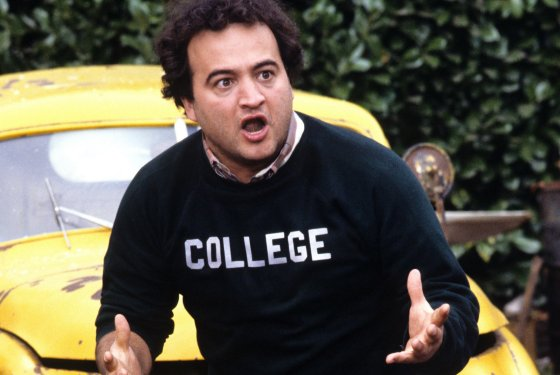
\includegraphics[max height = 0.3\textheight]{Images/belushicollege.jpg}
    }{}

    Please mute yourselves!
    \end{center}

    \ifthenelse{\equal{\thisSectionName}{Bonus}}
    {
        Get ready for some \emph{devilishly} hard questions!

        \vspace*{1em}
        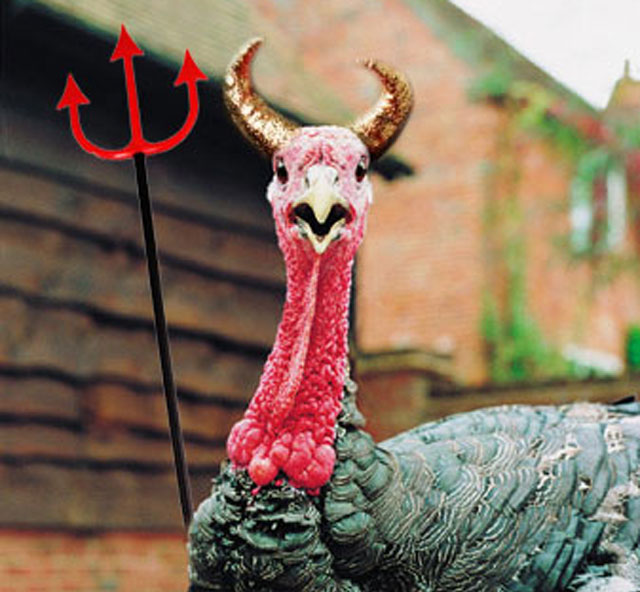
\includegraphics[max width=0.5\textwidth,
           max height=0.4\textheight]{Images/thankskilling-evil-turkey.jpg}
    }{}

    \vfill
  \end{frame}
}

\AtBeginSubsection[]{
  \begin{frame}
    \vfill
    \centering
    \begin{beamercolorbox}[sep=8pt,center,shadow=true,rounded=true]{title}
    \usebeamerfont{title}\insertsectionhead\par%
    \usebeamerfont{subtitle}\insertsubsectionhead\par%
    \end{beamercolorbox}
    \ifthenelse{\equal{\subsecname}{Answers}} {
        \begin{center}
        Unmute yourselves!
        \end{center}
    }
    \vfill
  \end{frame}
}
\begin{document}

\title{Welcome to Quarantine Trivia XII -- Thanksgiving Edition!}
\date{}

\begin{frame}
\titlepage{}
\begin{center}

\includegraphics[max width=0.9\textwidth,
    max height=0.4\textheight]{Images/triviatitleframelogo.png}
\end{center}
\end{frame}
\begin{frame}
In the spirit of the season, when we see so many images of the first Thanksgiving, we had our crack research team search for an image of the first trivia game. After a lot of hard work, they managed to find one.
\pause
\begin{center}
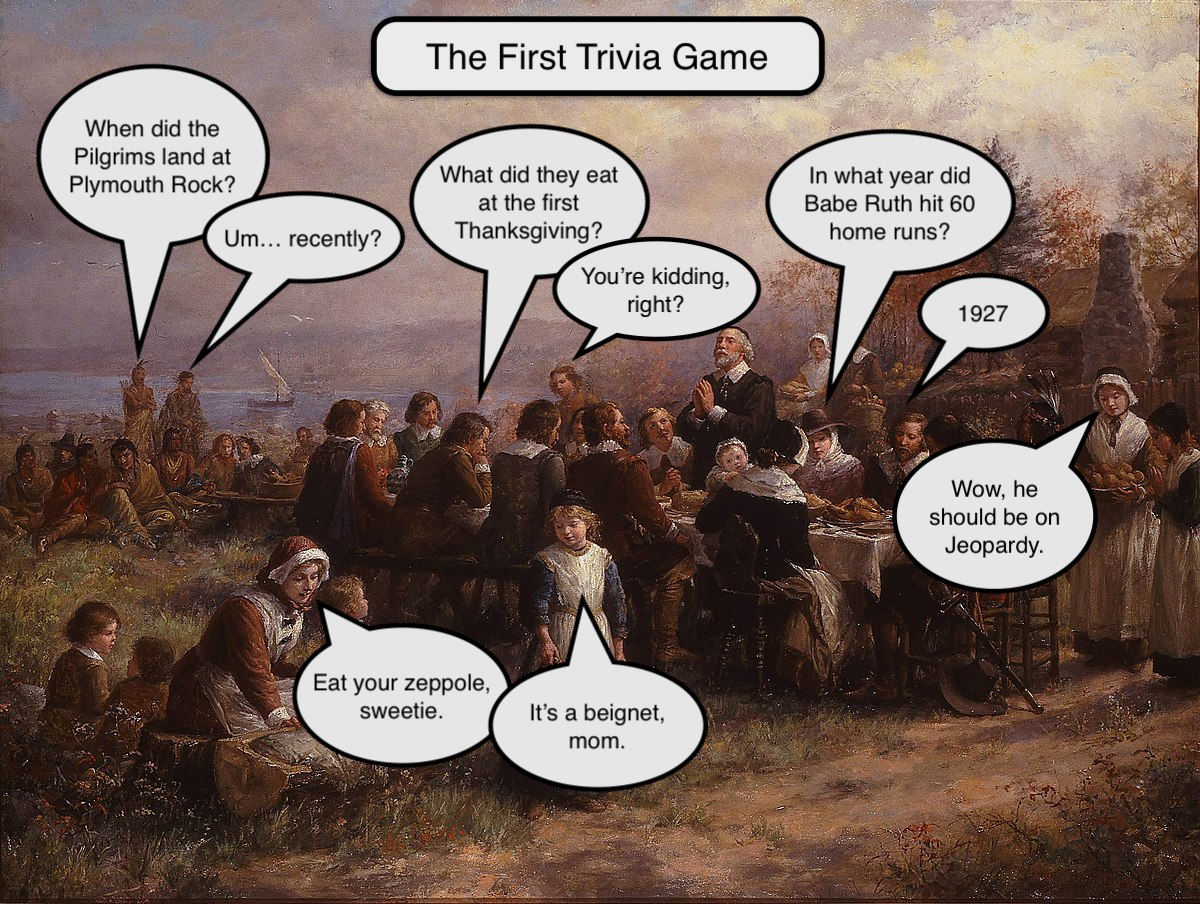
\includegraphics[max width=.9\textwidth,
max height=0.9\textheight]{Images/firstthanksgiving.jpg}
\end{center}
\end{frame}

\begingroup{}
\begingroup{}
\begin{frame}[t]{Categories}
This week, you'll be answering questions in the following categories:
\begin{enumerate}
\item Colorful Songs
\item Famous Animals in Fact and Fiction
\item Famous Court Cases
\item Biden/Harris
\item The Holiday Season
\item Scientific Breakthroughs
\item The Oldest\ldots
\item Shakespeare
\item Colorful Movies
\item Alex Trebek
\item Bonus Round
\end{enumerate}
\end{frame}
\endgroup{}

\begingroup{}
\begin{frame}
\vfill{}
\begin{beamercolorbox}[sep=8pt,center,shadow=true,rounded=true]{title}
\usebeamerfont{title}Good luck everyone! And have fun!
\end{beamercolorbox}
\vfill{}
\end{frame}
\endgroup{}
\def\thisSectionName{Colorful Songs}
\section{Round 1}
\subsection*{Q1}
\begin{frame}[t]{Round 1 --- Colorful Songs --- \mbox{Question 1}}
\vspace{-0.5em}
\begin{block}{Question}
What colorful song came up in connection with Brett Kavanaugh's Supreme Court confirmation hearing?
\end{block}
\end{frame}
\subsection*{Q2}
\begin{frame}[t]{Round 1 --- Colorful Songs --- \mbox{Question 2}}
\vspace{-0.5em}
\begin{block}{Question}
What colorful song was a hit for the Moody Blues in 1967?
\end{block}
\end{frame}
\subsection*{Q3}
\begin{frame}[t]{Round 1 --- Colorful Songs --- \mbox{Question 3}}
\vspace{-0.5em}
\begin{block}{Question}
What was the color of the Corvette that Prince sang about?
\end{block}
\end{frame}
\subsection*{Q4}
\begin{frame}[t]{Round 1 --- Colorful Songs --- \mbox{Question 4}}
\vspace{-0.5em}
\begin{block}{Question}
Which colorful Jay-Z song lent its name to the album it was on? (The album has had two similarly-named sequels.)
\end{block}
\end{frame}
\subsection*{Q5}
\begin{frame}[t]{Round 1 --- Colorful Songs --- \mbox{Question 5}}
\vspace{-0.5em}
\begin{block}{Question}
What colorful song did both Elvis and Carl Perkins sing to tell people to steer clear of their footwear?
\end{block}
\end{frame}
\subsection*{Q6}
\begin{frame}[t]{Round 1 --- Colorful Songs --- \mbox{Question 6}}
\vspace{-0.5em}
\begin{block}{Question}
Finish this line from the colorful novelty-song  lyrics: ``It was a one-eyed, one-horned, flying\ldots''
\end{block}
\end{frame}
\subsection*{Q7}
\begin{frame}[t]{Round 1 --- Colorful Songs --- \mbox{Question 7}}
\vspace{-0.5em}
\begin{block}{Question}
Which colorful Kanye West song featured Jamie Foxx and began with the lyric ``She take my money''?
\end{block}
\end{frame}
\subsection*{Q8}
\begin{frame}[t]{Round 1 --- Colorful Songs --- \mbox{Question 8}}
\vspace{-0.5em}
\begin{block}{Question}
John Legend and Lorde have both released songs with the same colorful title. What is the common title of these two songs?
\end{block}
\end{frame}
\subsection*{Q9}
\begin{frame}[t]{Round 1 --- Colorful Songs --- \mbox{Question 9}}
\vspace{-0.5em}
\begin{block}{Question}
Name either Beatles song whose title mentions a colorful bird.
\end{block}
\end{frame}
\subsection*{Q10}
\begin{frame}[t]{Round 1 --- Colorful Songs --- \mbox{Question 10}}
\vspace{-0.5em}
\begin{block}{Question}
What colorful animal gave its name to the title of a Kendrick Lamar song?
\end{block}
\end{frame}
\subsection{Answers}
\begin{frame}[t]{Round 1 --- Colorful Songs --- \mbox{Answer 1}}
\vspace{-0.5em}
\begin{block}{Question}
What colorful song came up in connection with Brett Kavanaugh's Supreme Court confirmation hearing?
\end{block}

\visible<2->{
    \begin{columns}[T,totalwidth=\linewidth]
    \begin{column}{0.32\linewidth}
    \begin{block}{Answer}
    \emph{Red Red Wine} (by UB40)
    \end{block}
    \end{column}
    \begin{column}{0.65\linewidth}
    \begin{center}
    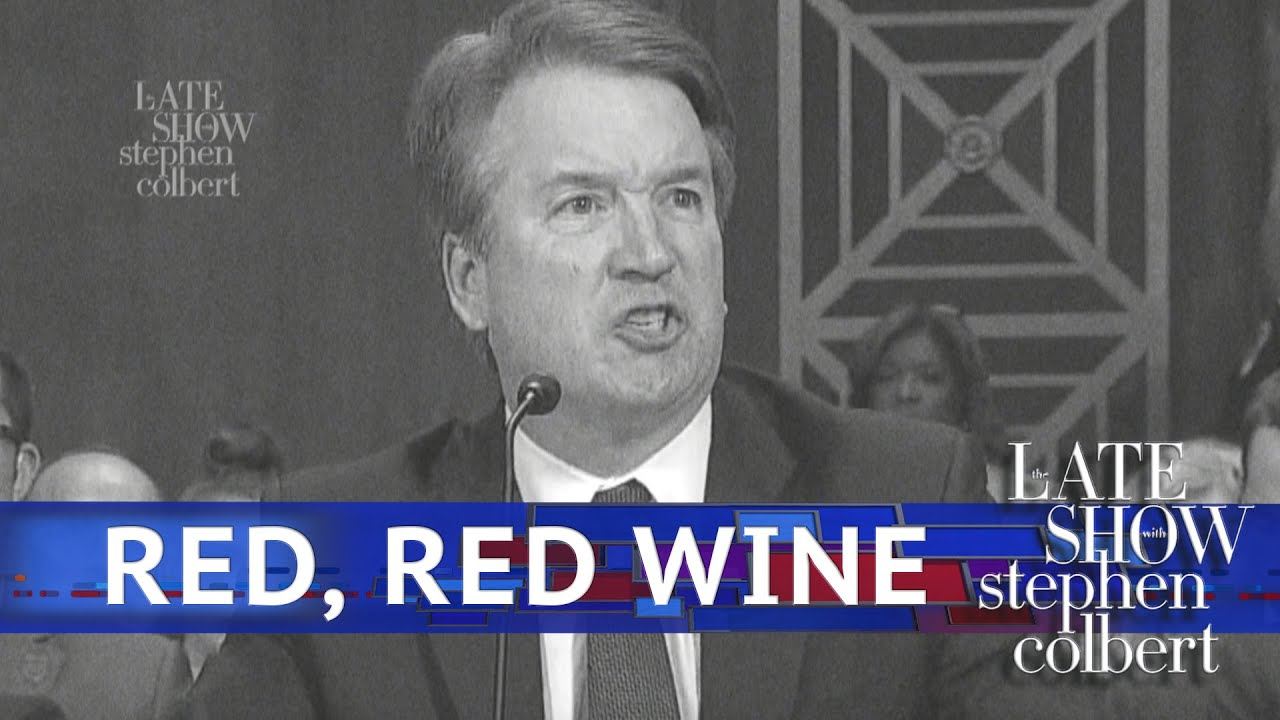
\includegraphics[max width=0.95\textwidth,
        max height=0.53000\textheight]{{Images/kredredwine}.jpg}
    \end{center}
    \end{column}
    \end{columns}
}
\end{frame}
\begin{frame}[t]{Round 1 --- Colorful Songs --- \mbox{Answer 2}}
\vspace{-0.5em}
\begin{block}{Question}
What colorful song was a hit for the Moody Blues in 1967?
\end{block}

\visible<2->{
    \begin{columns}[T,totalwidth=\linewidth]
    \begin{column}{0.32\linewidth}
    \begin{block}{Answer}
    \emph{Knights in White Satin}
    \end{block}
    \end{column}
    \begin{column}{0.65\linewidth}
    \begin{center}
    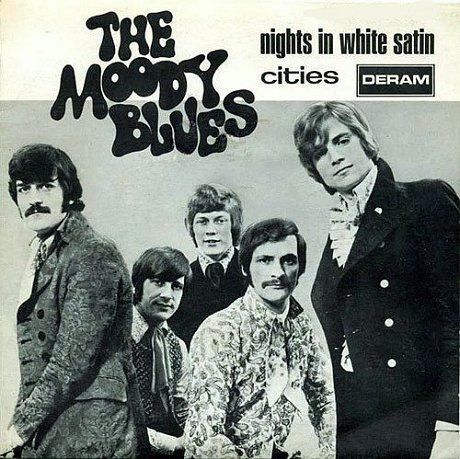
\includegraphics[max width=0.95\textwidth,
        max height=0.53000\textheight]{{Images/knightsinwhitesatin}.jpg}
    \end{center}
    \end{column}
    \end{columns}
}
\end{frame}
\begin{frame}[t]{Round 1 --- Colorful Songs --- \mbox{Answer 3}}
\vspace{-0.5em}
\begin{block}{Question}
What was the color of the Corvette that Prince sang about?
\end{block}

\visible<2->{
    \begin{columns}[T,totalwidth=\linewidth]
    \begin{column}{0.32\linewidth}
    \begin{block}{Answer}
    Red (\emph{Little Red Corvette})
    \end{block}
    \end{column}
    \begin{column}{0.65\linewidth}
    \begin{center}
    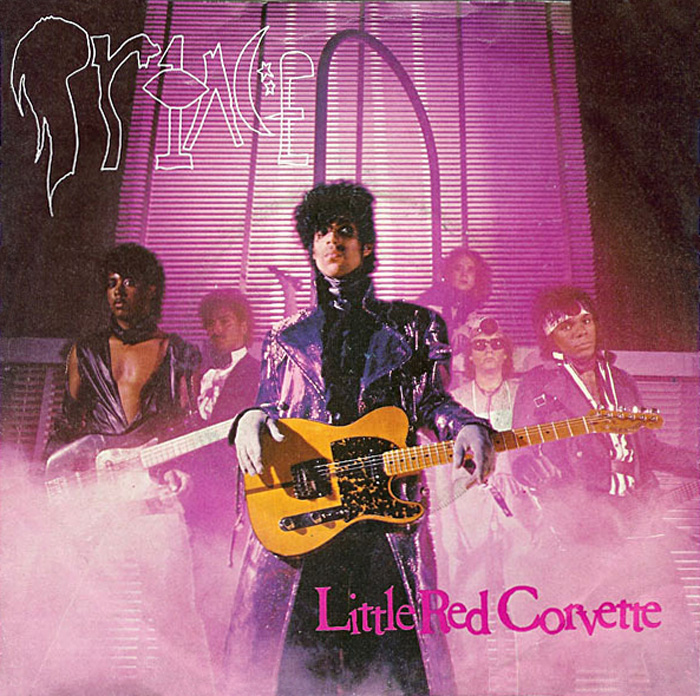
\includegraphics[max width=0.95\textwidth,
        max height=0.53000\textheight]{{Images/prince-little-red-corvette-warner-brothers}.jpg}
    \end{center}
    \end{column}
    \end{columns}
}
\end{frame}
\begin{frame}[t]{Round 1 --- Colorful Songs --- \mbox{Answer 4}}
\vspace{-0.5em}
\begin{block}{Question}
Which colorful Jay-Z song lent its name to the album it was on? (The album has had two similarly-named sequels.)
\end{block}

\visible<2->{
    \begin{columns}[T,totalwidth=\linewidth]
    \begin{column}{0.32\linewidth}
    \begin{block}{Answer}
    \emph{Blueprint}
    \end{block}
    \end{column}
    \begin{column}{0.65\linewidth}
    \begin{center}
    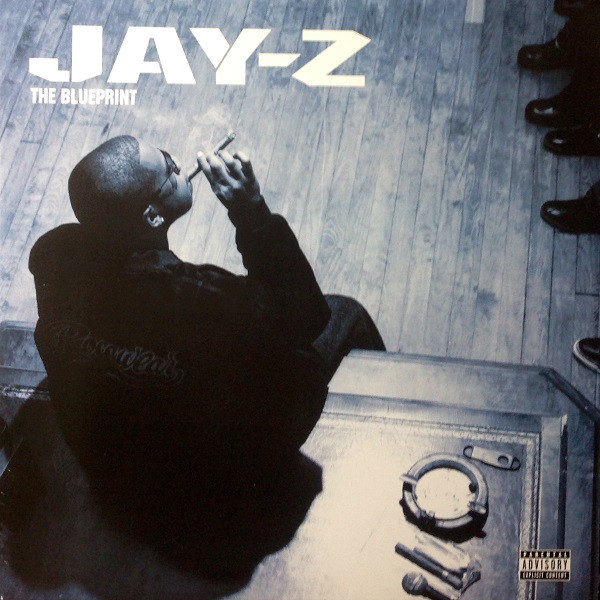
\includegraphics[max width=0.95\textwidth,
        max height=0.48000\textheight]{{Images/blueprint}.jpg}
    \end{center}
    \end{column}
    \end{columns}
}
\end{frame}
\begin{frame}[t]{Round 1 --- Colorful Songs --- \mbox{Answer 5}}
\vspace{-0.5em}
\begin{block}{Question}
What colorful song did both Elvis and Carl Perkins sing to tell people to steer clear of their footwear?
\end{block}

\visible<2->{
    \begin{columns}[T,totalwidth=\linewidth]
    \begin{column}{0.32\linewidth}
    \begin{block}{Answer}
    \emph{Blue Suede Shoes}
    \end{block}
    \end{column}
    \begin{column}{0.65\linewidth}
    \begin{center}
    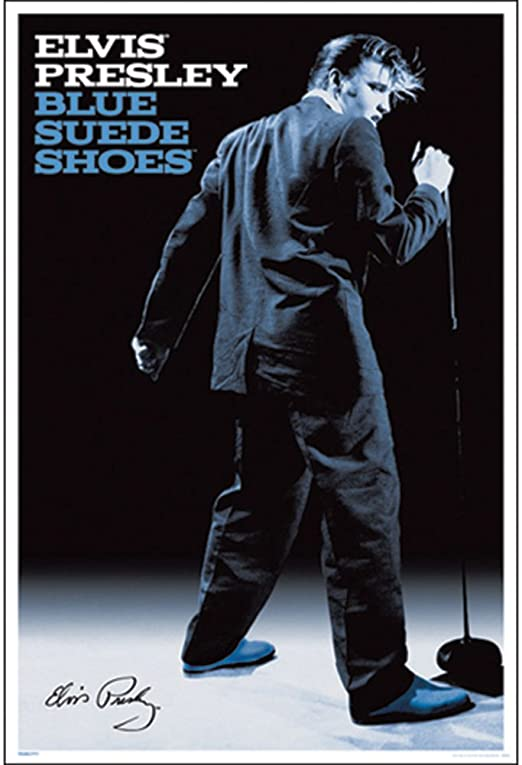
\includegraphics[max width=0.95\textwidth,
        max height=0.48000\textheight]{{Images/bluesuede}.jpg}
    \end{center}
    \end{column}
    \end{columns}
}
\end{frame}
\begin{frame}[t]{Round 1 --- Colorful Songs --- \mbox{Answer 6}}
\vspace{-0.5em}
\begin{block}{Question}
Finish this line from the colorful novelty-song  lyrics: ``It was a one-eyed, one-horned, flying\ldots''
\end{block}

\visible<2->{
    \begin{columns}[T,totalwidth=\linewidth]
    \begin{column}{0.32\linewidth}
    \begin{block}{Answer}
    Purple People Eater (from the song of the same name)
    \end{block}
    \end{column}
    \begin{column}{0.65\linewidth}
    \begin{center}
    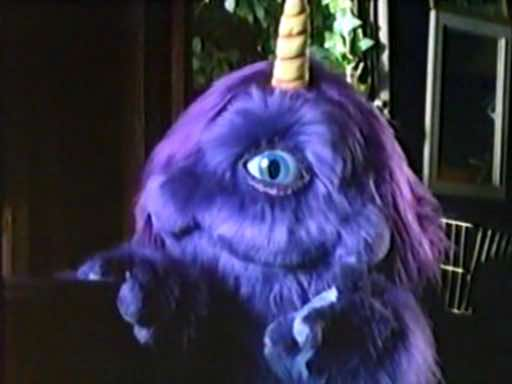
\includegraphics[max width=0.95\textwidth,
        max height=0.48000\textheight]{{Images/PPE2}.jpg}
    \end{center}
    \end{column}
    \end{columns}
}
\end{frame}
\begin{frame}[t]{Round 1 --- Colorful Songs --- \mbox{Answer 7}}
\vspace{-0.5em}
\begin{block}{Question}
Which colorful Kanye West song featured Jamie Foxx and began with the lyric ``She take my money''?
\end{block}

\visible<2->{
    \begin{columns}[T,totalwidth=\linewidth]
    \begin{column}{0.32\linewidth}
    \begin{block}{Answer}
    \emph{Gold Digger}
    \end{block}
    \end{column}
    \begin{column}{0.65\linewidth}
    \begin{center}
    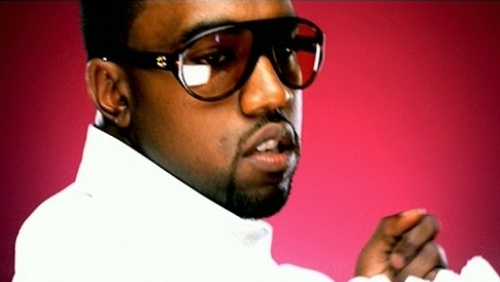
\includegraphics[max width=0.95\textwidth,
        max height=0.53000\textheight]{{Images/kanye-west-gold-digger}.jpg}
    \end{center}
    \end{column}
    \end{columns}
}
\end{frame}
\begin{frame}[t]{Round 1 --- Colorful Songs --- \mbox{Answer 8}}
\vspace{-0.5em}
\begin{block}{Question}
John Legend and Lorde have both released songs with the same colorful title. What is the common title of these two songs?
\end{block}

\visible<2->{
    \begin{columns}[T,totalwidth=\linewidth]
    \begin{column}{0.32\linewidth}
    \begin{block}{Answer}
    \emph{Green Light}
    \end{block}
    \end{column}
    \begin{column}{0.65\linewidth}
    \begin{center}
    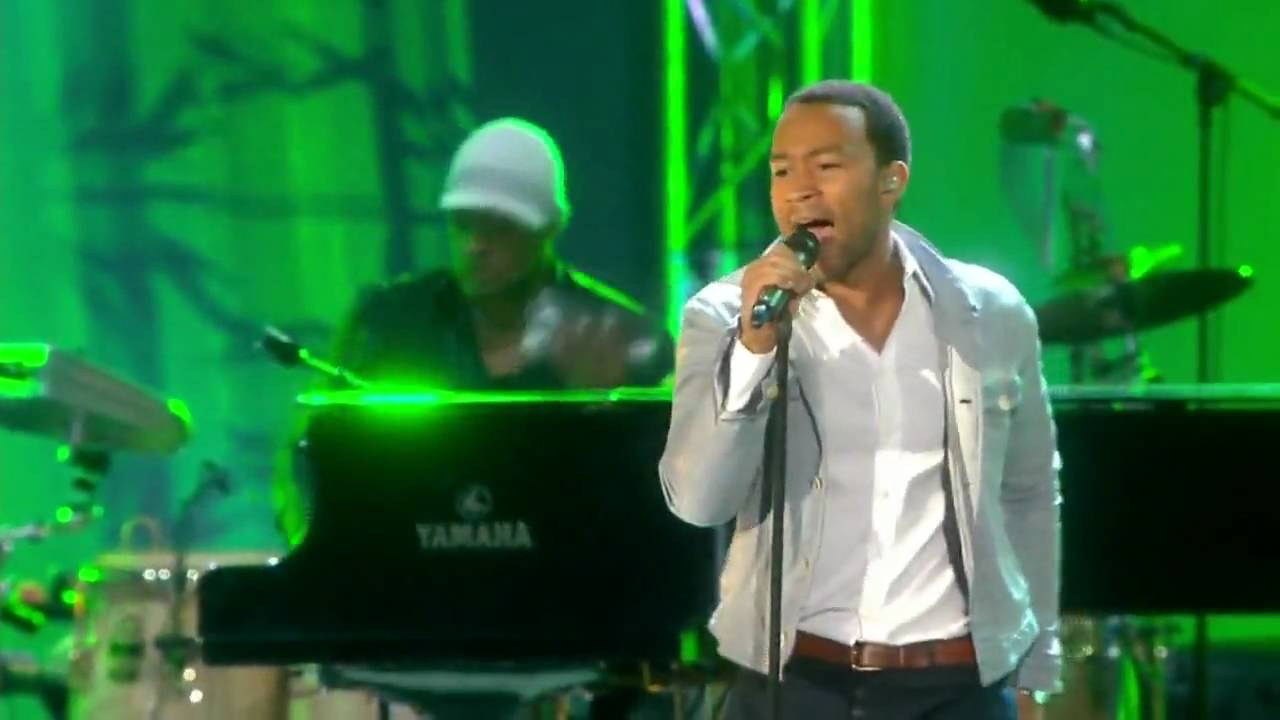
\includegraphics[max width=0.95\textwidth,
        max height=0.48000\textheight]{{Images/legendgreen}.jpg}
    \end{center}
    \end{column}
    \end{columns}
}
\end{frame}
\begin{frame}[t]{Round 1 --- Colorful Songs --- \mbox{Answer 9}}
\vspace{-0.5em}
\begin{block}{Question}
Name either Beatles song whose title mentions a colorful bird.
\end{block}

\visible<2->{
    \begin{columns}[T,totalwidth=\linewidth]
    \begin{column}{0.32\linewidth}
    \begin{block}{Answer}
    \emph{Blackbird} and \emph{Blue Jay Way} (you only needed one)
    \end{block}
    \end{column}
    \begin{column}{0.65\linewidth}
    \begin{center}
    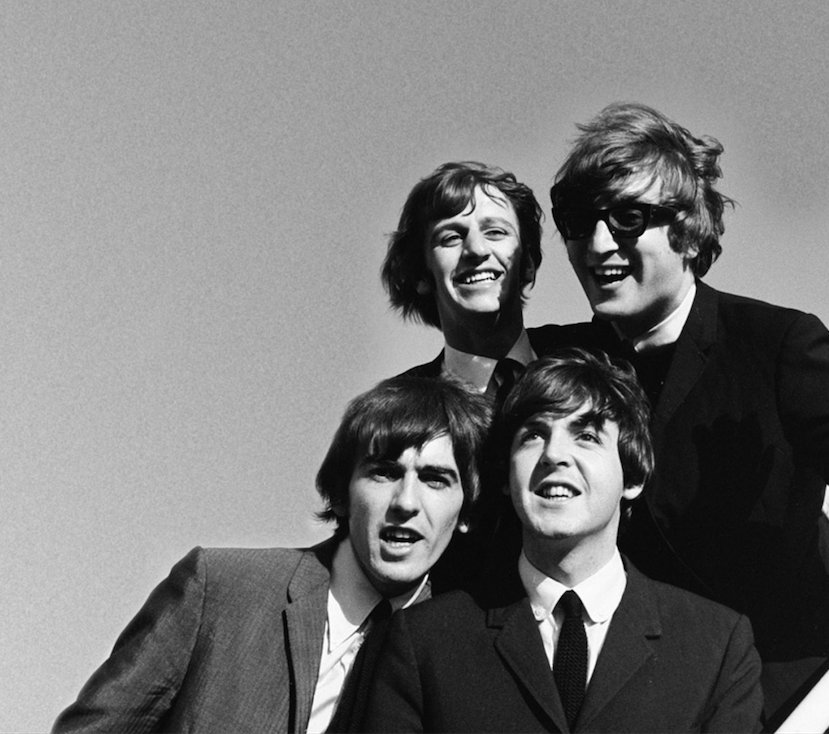
\includegraphics[max width=0.95\textwidth,
        max height=0.53000\textheight]{{Images/beatlesblackbird}.jpg}
    \end{center}
    \end{column}
    \end{columns}
}
\end{frame}
\begin{frame}[t]{Round 1 --- Colorful Songs --- \mbox{Answer 10}}
\vspace{-0.5em}
\begin{block}{Question}
What colorful animal gave its name to the title of a Kendrick Lamar song?
\end{block}

\visible<2->{
    \begin{columns}[T,totalwidth=\linewidth]
    \begin{column}{0.32\linewidth}
    \begin{block}{Answer}
    \emph{Black Panther}
    \end{block}
    \end{column}
    \begin{column}{0.65\linewidth}
    \begin{center}
    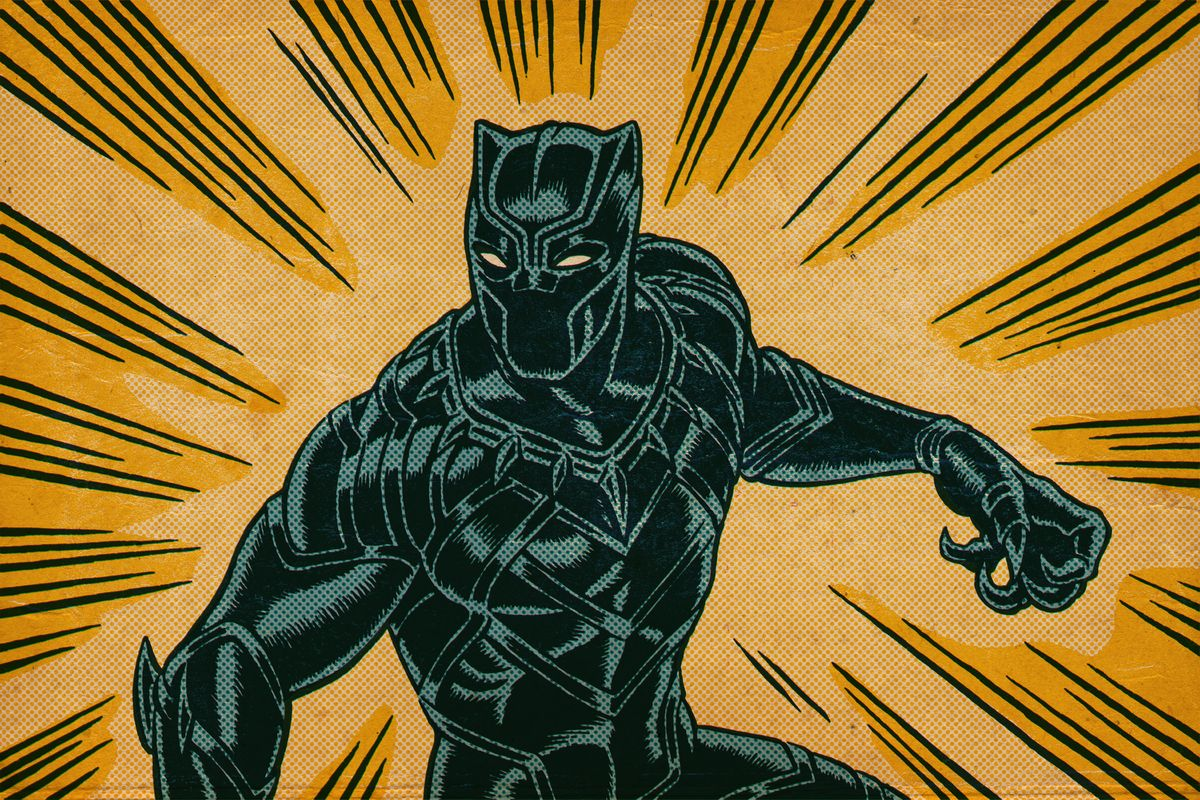
\includegraphics[max width=0.95\textwidth,
        max height=0.53000\textheight]{{Images/blackpanther}.jpg}
    \end{center}
    \end{column}
    \end{columns}
}
\end{frame}
\def\thisSectionName{Famous Animals in Fact and Fiction}
\section{Round 2}
\subsection*{Q1}
\begin{frame}[t]{Round 2 --- Famous Animals in Fact and Fiction --- \mbox{Question 1}}
\vspace{-0.5em}
\begin{columns}[T,totalwidth=\linewidth]
\begin{column}{0.32\linewidth}
\begin{block}{Question}
The fish pictured here was the main character of which children's book?
\end{block}
\end{column}
\begin{column}{0.65\linewidth}
\begin{center}
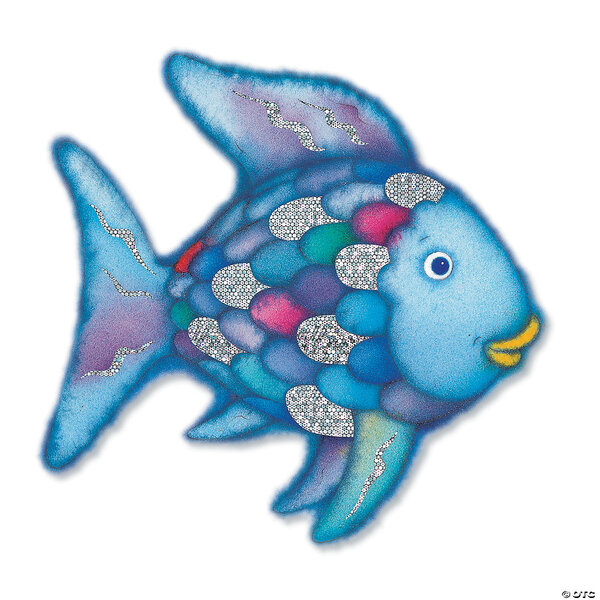
\includegraphics[max width=0.95\textwidth,max height=0.7\textheight]{{Images/rainbowfish}.jpeg}
\end{center}
\end{column}
\end{columns}
\end{frame}
\subsection*{Q2}
\begin{frame}[t]{Round 2 --- Famous Animals in Fact and Fiction --- \mbox{Question 2}}
\vspace{-0.5em}
\begin{block}{Question}
What was the name of the sheep who was the first mammal to be cloned?
\end{block}
\end{frame}
\subsection*{Q3}
\begin{frame}[t]{Round 2 --- Famous Animals in Fact and Fiction --- \mbox{Question 3}}
\vspace{-0.5em}
\begin{block}{Question}
What is the two-word name of the Pennsylvanian groundhog who each February determines whether or not we will have six more weeks of winter? 
\end{block}
\end{frame}
\subsection*{Q4}
\begin{frame}[t]{Round 2 --- Famous Animals in Fact and Fiction --- \mbox{Question 4}}
\vspace{-0.5em}
\begin{block}{Question}
What is the name of the cricket in Disney's \emph{Pinocchio}?
\end{block}
\end{frame}
\subsection*{Q5}
\begin{frame}[t]{Round 2 --- Famous Animals in Fact and Fiction --- \mbox{Question 5}}
\vspace{-0.5em}
\begin{block}{Question}
In \emph{The Legend of Sleepy Hollow}, what is the name of Ichabod Crane's horse?
\end{block}
\end{frame}
\subsection*{Q6}
\begin{frame}[t]{Round 2 --- Famous Animals in Fact and Fiction --- \mbox{Question 6}}
\vspace{-0.5em}
\begin{columns}[T,totalwidth=\linewidth]
\begin{column}{0.32\linewidth}
\begin{block}{Question}
What was the name of the famous dog who was part of the team that saved Nome, Alaska, by delivering diphtheria antidote to that city? (There is a statue of this famous canine in Central Park.)
\end{block}
\end{column}
\begin{column}{0.65\linewidth}
\begin{center}
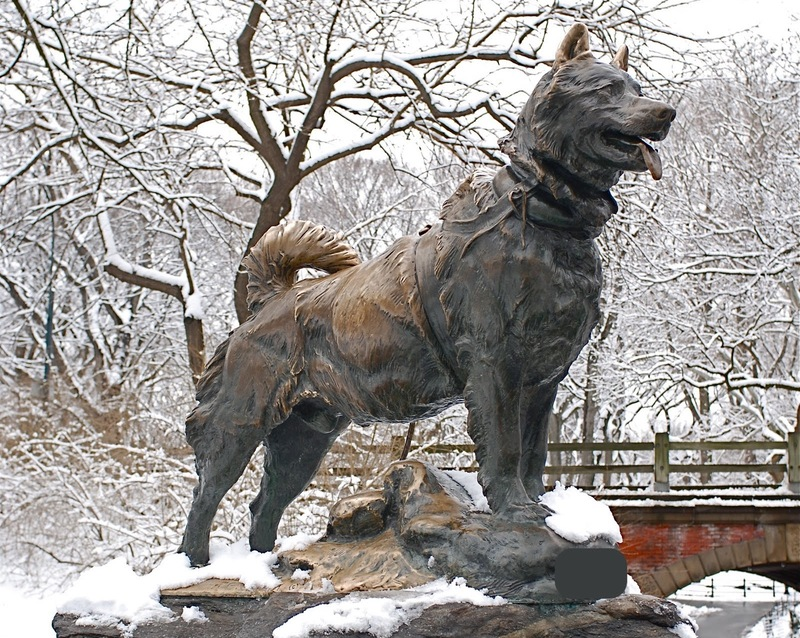
\includegraphics[max width=0.95\textwidth,max height=0.7\textheight]{{Images/balto}.JPG}
\end{center}
\end{column}
\end{columns}
\end{frame}
\subsection*{Q7}
\begin{frame}[t]{Round 2 --- Famous Animals in Fact and Fiction --- \mbox{Question 7}}
\vspace{-0.5em}
\begin{block}{Question}
What was the name of the first ``first dog'' under Barack Obama? (The Obamas adopted a second dog in 2013.)
\end{block}
\end{frame}
\subsection*{Q8}
\begin{frame}[t]{Round 2 --- Famous Animals in Fact and Fiction --- \mbox{Question 8}}
\vspace{-0.5em}
\begin{block}{Question}
What was the name of the fictional bull terrier who was part of a Bud Light marketing campaign in the 1980s?
\end{block}
\end{frame}
\subsection*{Q9}
\begin{frame}[t]{Round 2 --- Famous Animals in Fact and Fiction --- \mbox{Question 9}}
\vspace{-0.5em}
\begin{block}{Question}
Whose cow was purported to have started the Great Chicago Fire by kicking over a lantern? (The cow was exonerated by the Chicago City Council in 1997.)
\end{block}
\end{frame}
\subsection*{Q10}
\begin{frame}[t]{Round 2 --- Famous Animals in Fact and Fiction --- \mbox{Question 10}}
\vspace{-0.5em}
\begin{block}{Question}
What was the name of the German Shepherd who was rescued from a WWI battlefield and went on to star in 27 Hollywood films?
\end{block}
\end{frame}
\subsection{Answers}
\begin{frame}[t]{Round 2 --- Famous Animals in Fact and Fiction --- \mbox{Answer 1}}
\vspace{-0.5em}
\begin{columns}[T,totalwidth=\linewidth]
\begin{column}{0.32\linewidth}
\begin{block}{Question}
The fish pictured here was the main character of which children's book?
\end{block}
\visible<2->{
    \begin{block}{Answer}
    \emph{The Rainbow Fish}
    \end{block}
}
\end{column}
\begin{column}{0.65\linewidth}
\begin{center}
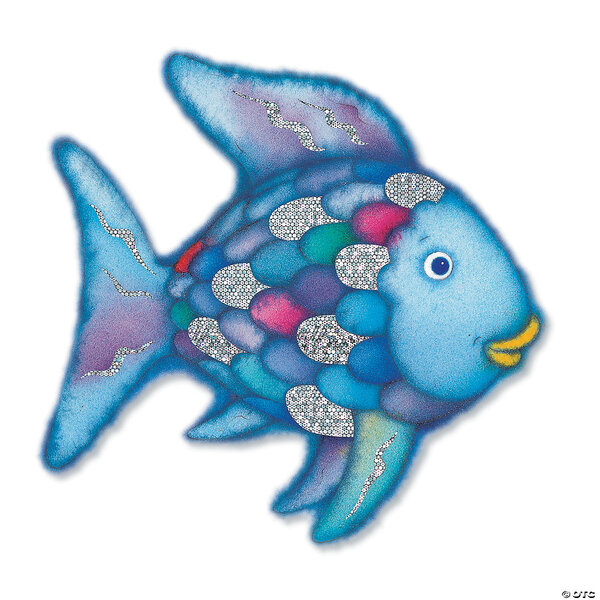
\includegraphics[max width=0.95\textwidth,max height=0.7\textheight]{{Images/rainbowfish}.jpeg}
\end{center}
\end{column}
\end{columns}
\end{frame}
\begin{frame}[t]{Round 2 --- Famous Animals in Fact and Fiction --- \mbox{Answer 2}}
\vspace{-0.5em}
\begin{block}{Question}
What was the name of the sheep who was the first mammal to be cloned?
\end{block}

\visible<2->{
    \begin{columns}[T,totalwidth=\linewidth]
    \begin{column}{0.32\linewidth}
    \begin{block}{Answer}
    Dolly
    \end{block}
    \end{column}
    \begin{column}{0.65\linewidth}
    \begin{center}
    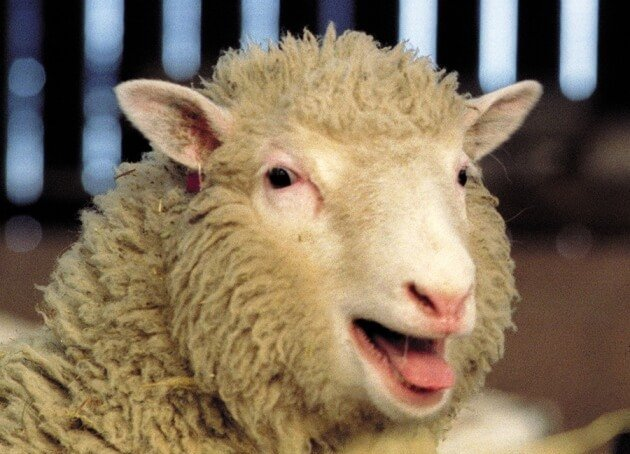
\includegraphics[max width=0.95\textwidth,
        max height=0.53000\textheight]{{Images/dolly}.jpg}
    \end{center}
    \end{column}
    \end{columns}
}
\end{frame}
\begin{frame}[t]{Round 2 --- Famous Animals in Fact and Fiction --- \mbox{Answer 3}}
\vspace{-0.5em}
\begin{block}{Question}
What is the two-word name of the Pennsylvanian groundhog who each February determines whether or not we will have six more weeks of winter? 
\end{block}

\visible<2->{
    \begin{columns}[T,totalwidth=\linewidth]
    \begin{column}{0.32\linewidth}
    \begin{block}{Answer}
    Punxsutawney Phil (we will be lenient with spelling)
    \end{block}
    \end{column}
    \begin{column}{0.65\linewidth}
    \begin{center}
    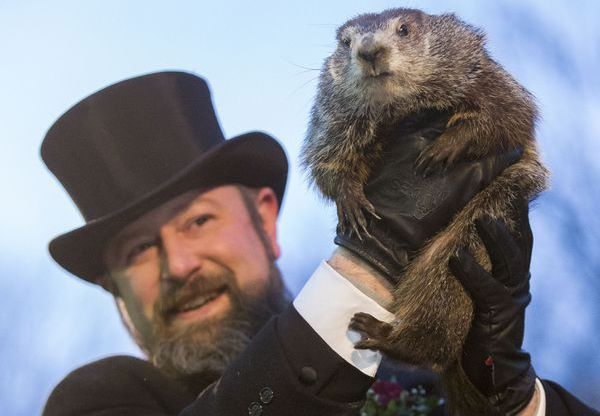
\includegraphics[max width=0.95\textwidth,
        max height=0.48000\textheight]{{Images/phil}.JPG}
    \end{center}
    \end{column}
    \end{columns}
}
\end{frame}
\begin{frame}[t]{Round 2 --- Famous Animals in Fact and Fiction --- \mbox{Answer 4}}
\vspace{-0.5em}
\begin{block}{Question}
What is the name of the cricket in Disney's \emph{Pinocchio}?
\end{block}

\visible<2->{
    \begin{columns}[T,totalwidth=\linewidth]
    \begin{column}{0.32\linewidth}
    \begin{block}{Answer}
    Jiminy Cricket
    \end{block}
    \end{column}
    \begin{column}{0.65\linewidth}
    \begin{center}
    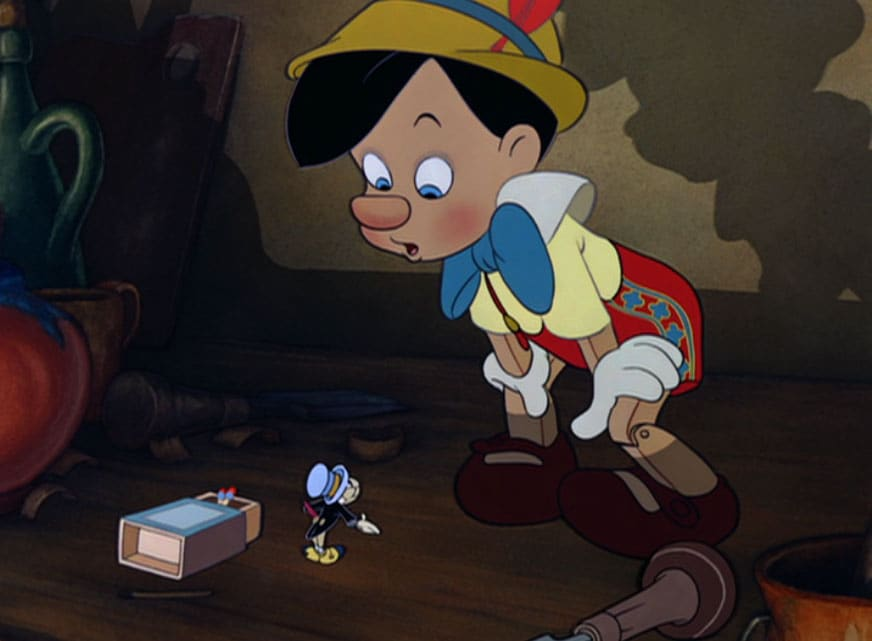
\includegraphics[max width=0.95\textwidth,
        max height=0.53000\textheight]{{Images/Jiminy-Cricket-46}.jpg}
    \end{center}
    \end{column}
    \end{columns}
}
\end{frame}
\begin{frame}[t]{Round 2 --- Famous Animals in Fact and Fiction --- \mbox{Answer 5}}
\vspace{-0.5em}
\begin{block}{Question}
In \emph{The Legend of Sleepy Hollow}, what is the name of Ichabod Crane's horse?
\end{block}

\visible<2->{
    \begin{columns}[T,totalwidth=\linewidth]
    \begin{column}{0.32\linewidth}
    \begin{block}{Answer}
    Gunpowder
    \end{block}
    \end{column}
    \begin{column}{0.65\linewidth}
    \begin{center}
    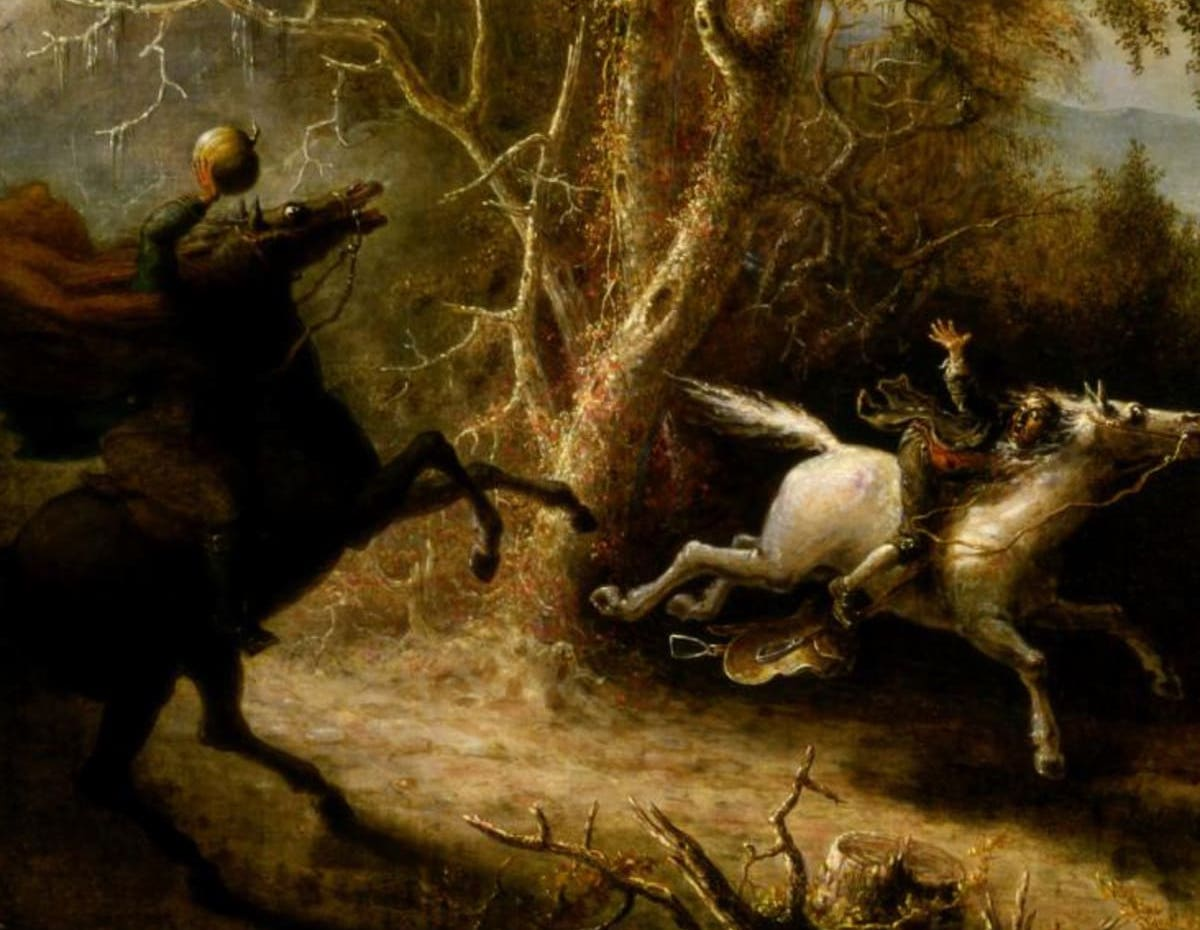
\includegraphics[max width=0.95\textwidth,
        max height=0.53000\textheight]{{Images/sleepyhollow}.jpg}
    \end{center}
    \end{column}
    \end{columns}
}
\end{frame}
\begin{frame}[t]{Round 2 --- Famous Animals in Fact and Fiction --- \mbox{Answer 6}}
\vspace{-0.5em}
\begin{block}{Question}
What was the name of the famous dog who was part of the team that saved Nome, Alaska, by delivering diphtheria antidote to that city? (There is a statue of this famous canine in Central Park.)
\end{block}

\visible<2->{
    \begin{columns}[T,totalwidth=\linewidth]
    \begin{column}{0.25\linewidth}
    \begin{block}{Answer}
    Balto
    \end{block}
    \end{column}
    \begin{column}{0.7\linewidth}
    \begin{center}
    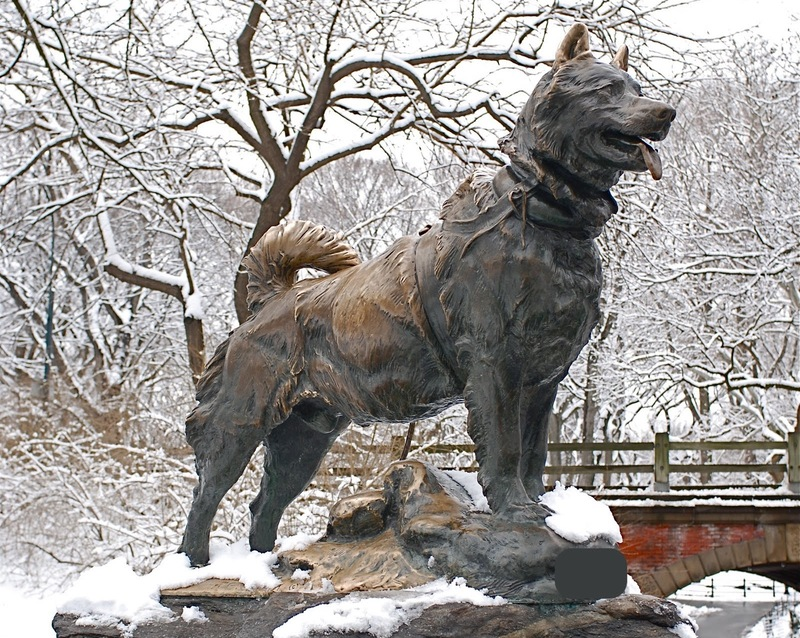
\includegraphics[max height=0.5\textheight]{{Images/balto}.JPG}
    \end{center}
    \end{column}
    \end{columns}
}
\end{frame}
\begin{frame}[t]{Round 2 --- Famous Animals in Fact and Fiction --- \mbox{Answer 7}}
\vspace{-0.5em}
\begin{block}{Question}
What was the name of the first ``first dog'' under Barack Obama? (The Obamas adopted a second dog in 2013.)
\end{block}

\visible<2->{
    \begin{columns}[T,totalwidth=\linewidth]
    \begin{column}{0.32\linewidth}
    \begin{block}{Answer}
    Bo
    \end{block}
    \end{column}
    \begin{column}{0.65\linewidth}
    \begin{center}
    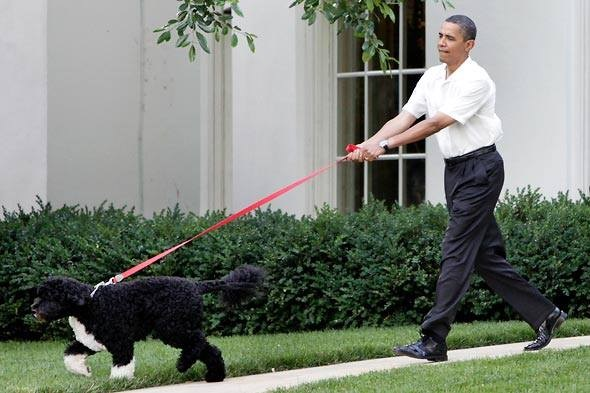
\includegraphics[max width=0.95\textwidth,
        max height=0.48000\textheight]{{Images/bo}.jpg}
    \end{center}
    \end{column}
    \end{columns}
}
\end{frame}
\begin{frame}[t]{Round 2 --- Famous Animals in Fact and Fiction --- \mbox{Answer 8}}
\vspace{-0.5em}
\begin{block}{Question}
What was the name of the fictional bull terrier who was part of a Bud Light marketing campaign in the 1980s?
\end{block}

\visible<2->{
    \begin{columns}[T,totalwidth=\linewidth]
    \begin{column}{0.32\linewidth}
    \begin{block}{Answer}
    Spuds MacKenzie
    \end{block}
    \end{column}
    \begin{column}{0.65\linewidth}
    \begin{center}
    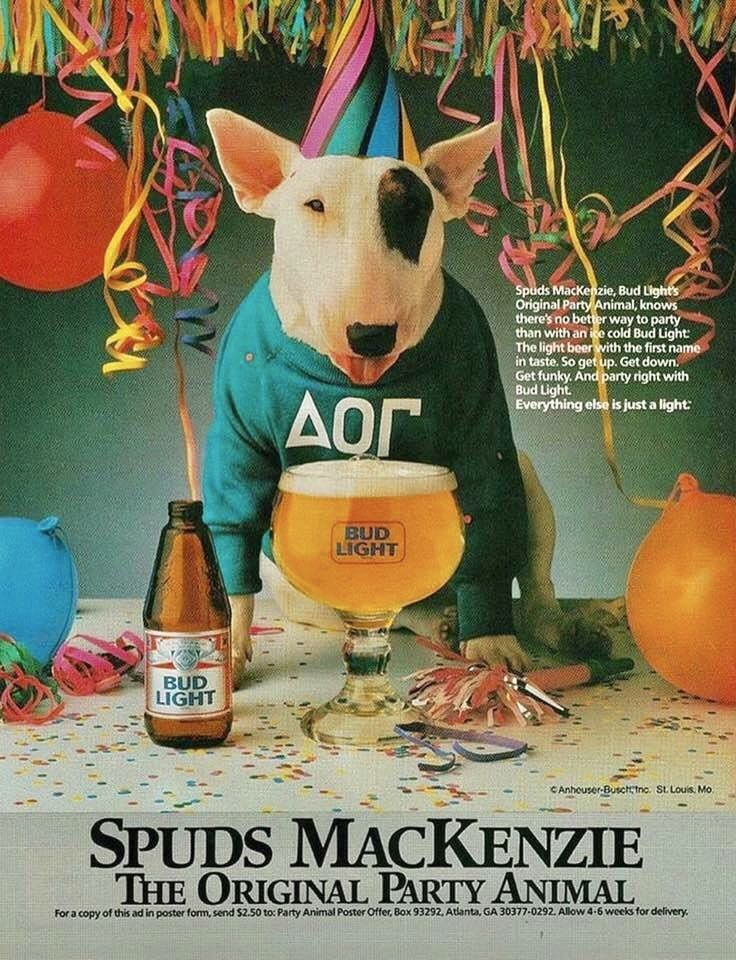
\includegraphics[max width=0.95\textwidth,
        max height=0.48000\textheight]{{Images/spuds}.jpg}
    \end{center}
    \end{column}
    \end{columns}
}
\end{frame}
\begin{frame}[t]{Round 2 --- Famous Animals in Fact and Fiction --- \mbox{Answer 9}}
\vspace{-0.5em}
\begin{block}{Question}
Whose cow was purported to have started the Great Chicago Fire by kicking over a lantern? (The cow was exonerated by the Chicago City Council in 1997.)
\end{block}

\visible<2->{
    \begin{columns}[T,totalwidth=\linewidth]
    \begin{column}{0.32\linewidth}
    \begin{block}{Answer}
    Mrs. O'Leary's Cow
    \end{block}
    \end{column}
    \begin{column}{0.65\linewidth}
    \begin{center}
    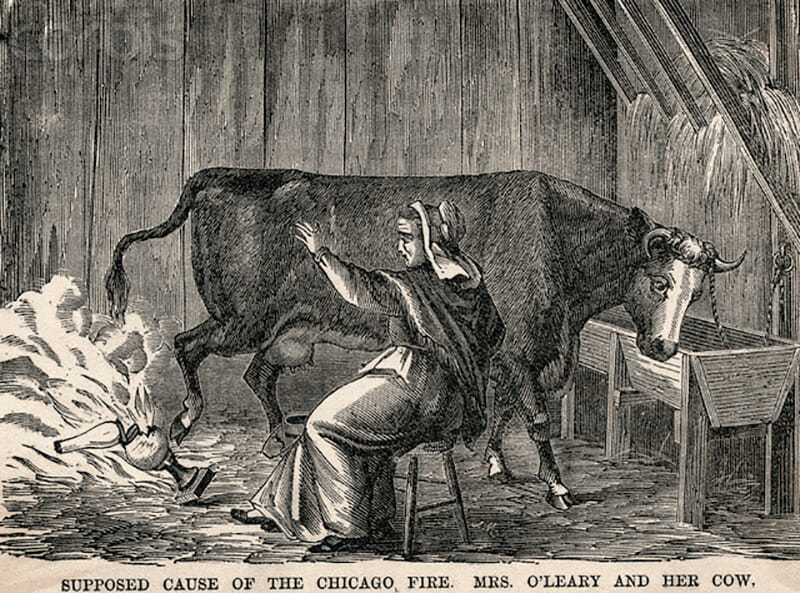
\includegraphics[max width=0.95\textwidth,
        max height=0.43000\textheight]{{Images/olearycaracature}.jpg}
    \end{center}
    \end{column}
    \end{columns}
}
\end{frame}
\begin{frame}[t]{Round 2 --- Famous Animals in Fact and Fiction --- \mbox{Answer 10}}
\vspace{-0.5em}
\begin{block}{Question}
What was the name of the German Shepherd who was rescued from a WWI battlefield and went on to star in 27 Hollywood films?
\end{block}

\visible<2->{
    \begin{columns}[T,totalwidth=\linewidth]
    \begin{column}{0.32\linewidth}
    \begin{block}{Answer}
    Rin-Tin-Tin
    \end{block}
    \end{column}
    \begin{column}{0.65\linewidth}
    \begin{center}
    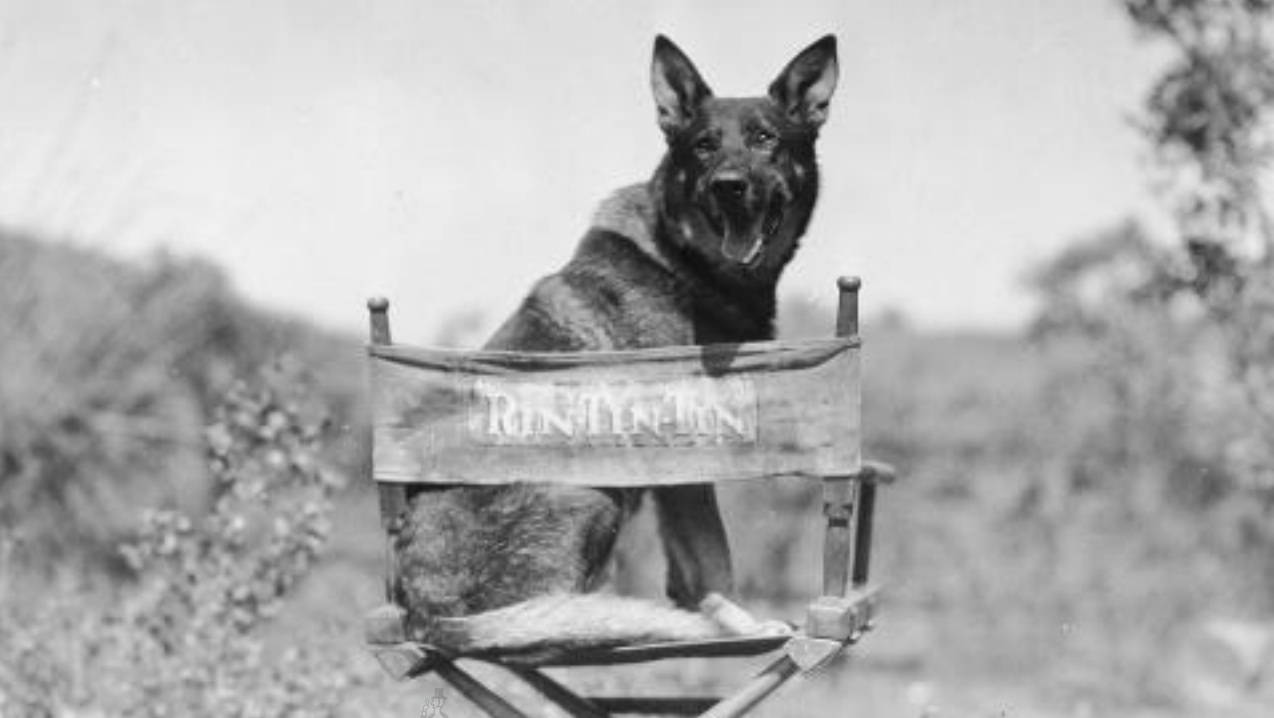
\includegraphics[max width=0.95\textwidth,
        max height=0.48000\textheight]{{Images/rintintin}.jpg}
    \end{center}
    \end{column}
    \end{columns}
}
\end{frame}
\def\thisSectionName{Famous Court Cases}
\section{Round 3}
\subsection*{Q1}
\begin{frame}[t]{Round 3 --- Famous Court Cases --- \mbox{Question 1}}
\vspace{-0.5em}
\begin{block}{Question}
The Supreme Court's decision in which case made same-sex marriage the law of the land?
\end{block}
\end{frame}
\subsection*{Q2}
\begin{frame}[t]{Round 3 --- Famous Court Cases --- \mbox{Question 2}}
\vspace{-0.5em}
\begin{block}{Question}
In which case did the Supreme Court hold that ``separate but equal'' schools were ``inherently unequal?''
\end{block}
\end{frame}
\subsection*{Q3}
\begin{frame}[t]{Round 3 --- Famous Court Cases --- \mbox{Question 3}}
\vspace{-0.5em}
\begin{block}{Question}
In which case did the Supreme Court hold that corporations and unions were people for purposes of their making campaign contributions?
\end{block}
\end{frame}
\subsection*{Q4}
\begin{frame}[t]{Round 3 --- Famous Court Cases --- \mbox{Question 4}}
\vspace{-0.5em}
\begin{block}{Question}
The Supreme Court's action in which case halted the recount in the 2000 presidential election?
\end{block}
\end{frame}
\subsection*{Q5}
\begin{frame}[t]{Round 3 --- Famous Court Cases --- \mbox{Question 5}}
\vspace{-0.5em}
\begin{block}{Question}
What court case about teaching evolution was known as the ``Monkey Trial?''
\end{block}
\end{frame}
\subsection*{Q6}
\begin{frame}[t]{Round 3 --- Famous Court Cases --- \mbox{Question 6}}
\vspace{-0.5em}
\begin{block}{Question}
What two newspapers were involved in the 1971 Pentagon Papers prior restraint case?
\end{block}
\end{frame}
\subsection*{Q7}
\begin{frame}[t]{Round 3 --- Famous Court Cases --- \mbox{Question 7}}
\vspace{-0.5em}
\begin{block}{Question}
In his dissent in  Schenck v. United States, Justice Holmes put forth his famous example of speech that is not protected by the First Amendment.  What was his example of such speech?
\end{block}
\end{frame}
\subsection*{Q8}
\begin{frame}[t]{Round 3 --- Famous Court Cases --- \mbox{Question 8}}
\vspace{-0.5em}
\begin{block}{Question}
In which case did the Supreme Court hold that when a person is arrested, he or she must be ``read their rights'' by the arresting officer?
\end{block}
\end{frame}
\subsection*{Q9}
\begin{frame}[t]{Round 3 --- Famous Court Cases --- \mbox{Question 9}}
\vspace{-0.5em}
\begin{block}{Question}
In which case did the Supreme Court hold that criminal defendants have the right to be represented by an  attorney at no cost? 
\end{block}
\end{frame}
\subsection*{Q10}
\begin{frame}[t]{Round 3 --- Famous Court Cases --- \mbox{Question 10}}
\vspace{-0.5em}
\begin{block}{Question}
In which case did the Supreme Court render its infamous decision upholding the government's internment of Americans of Japanese ancestry during World War II\@?
\end{block}
\end{frame}
\subsection{Answers}
\begin{frame}[t]{Round 3 --- Famous Court Cases --- \mbox{Answer 1}}
\vspace{-0.5em}
\begin{block}{Question}
The Supreme Court's decision in which case made same-sex marriage the law of the land?
\end{block}

\visible<2->{
    \begin{columns}[T,totalwidth=\linewidth]
    \begin{column}{0.32\linewidth}
    \begin{block}{Answer}
    Obergefell v. Hodges (2015)
    \end{block}
    \end{column}
    \begin{column}{0.65\linewidth}
    \begin{center}
    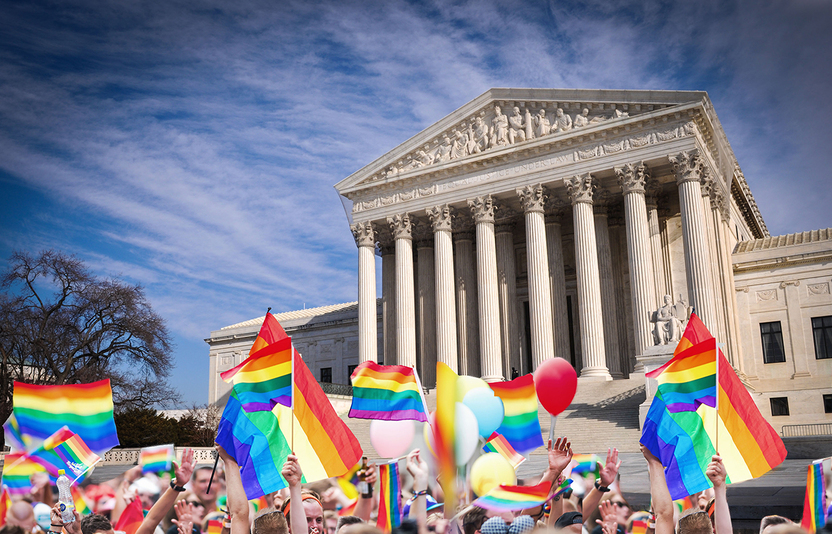
\includegraphics[max width=0.95\textwidth,
        max height=0.53000\textheight]{{Images/hodges}.jpg}
    \end{center}
    \end{column}
    \end{columns}
}
\end{frame}
\begin{frame}[t]{Round 3 --- Famous Court Cases --- \mbox{Answer 2}}
\vspace{-0.5em}
\begin{block}{Question}
In which case did the Supreme Court hold that ``separate but equal'' schools were ``inherently unequal?''
\end{block}

\visible<2->{
    \begin{columns}[T,totalwidth=\linewidth]
    \begin{column}{0.32\linewidth}
    \begin{block}{Answer}
    Brown v. Topeka Board of Education (1954)
    \end{block}
    \end{column}
    \begin{column}{0.65\linewidth}
    \begin{center}
    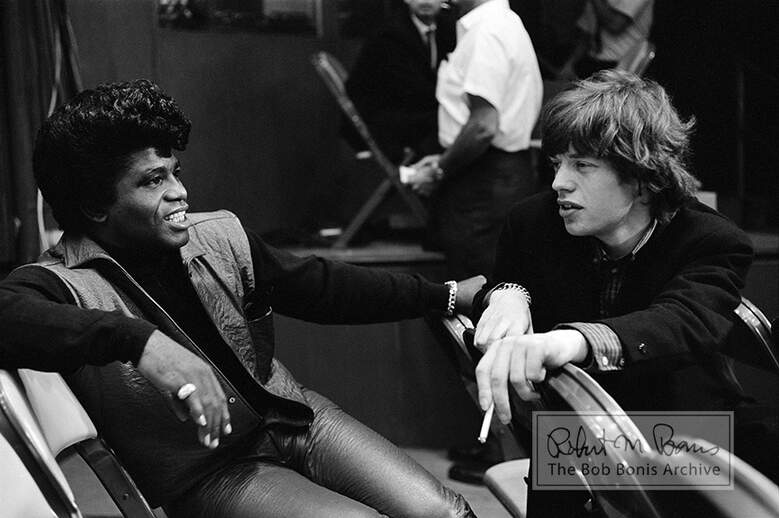
\includegraphics[max width=0.95\textwidth,
        max height=0.48000\textheight]{{Images/brown}.jpg}
    \end{center}
    \end{column}
    \end{columns}
}
\end{frame}
\begin{frame}[t]{Round 3 --- Famous Court Cases --- \mbox{Answer 3}}
\vspace{-0.5em}
\begin{block}{Question}
In which case did the Supreme Court hold that corporations and unions were people for purposes of their making campaign contributions?
\end{block}

\visible<2->{
    \begin{columns}[T,totalwidth=\linewidth]
    \begin{column}{0.32\linewidth}
    \begin{block}{Answer}
    Citizens United v. FEC (2010)
    \end{block}
    \end{column}
    \begin{column}{0.65\linewidth}
    \begin{center}
    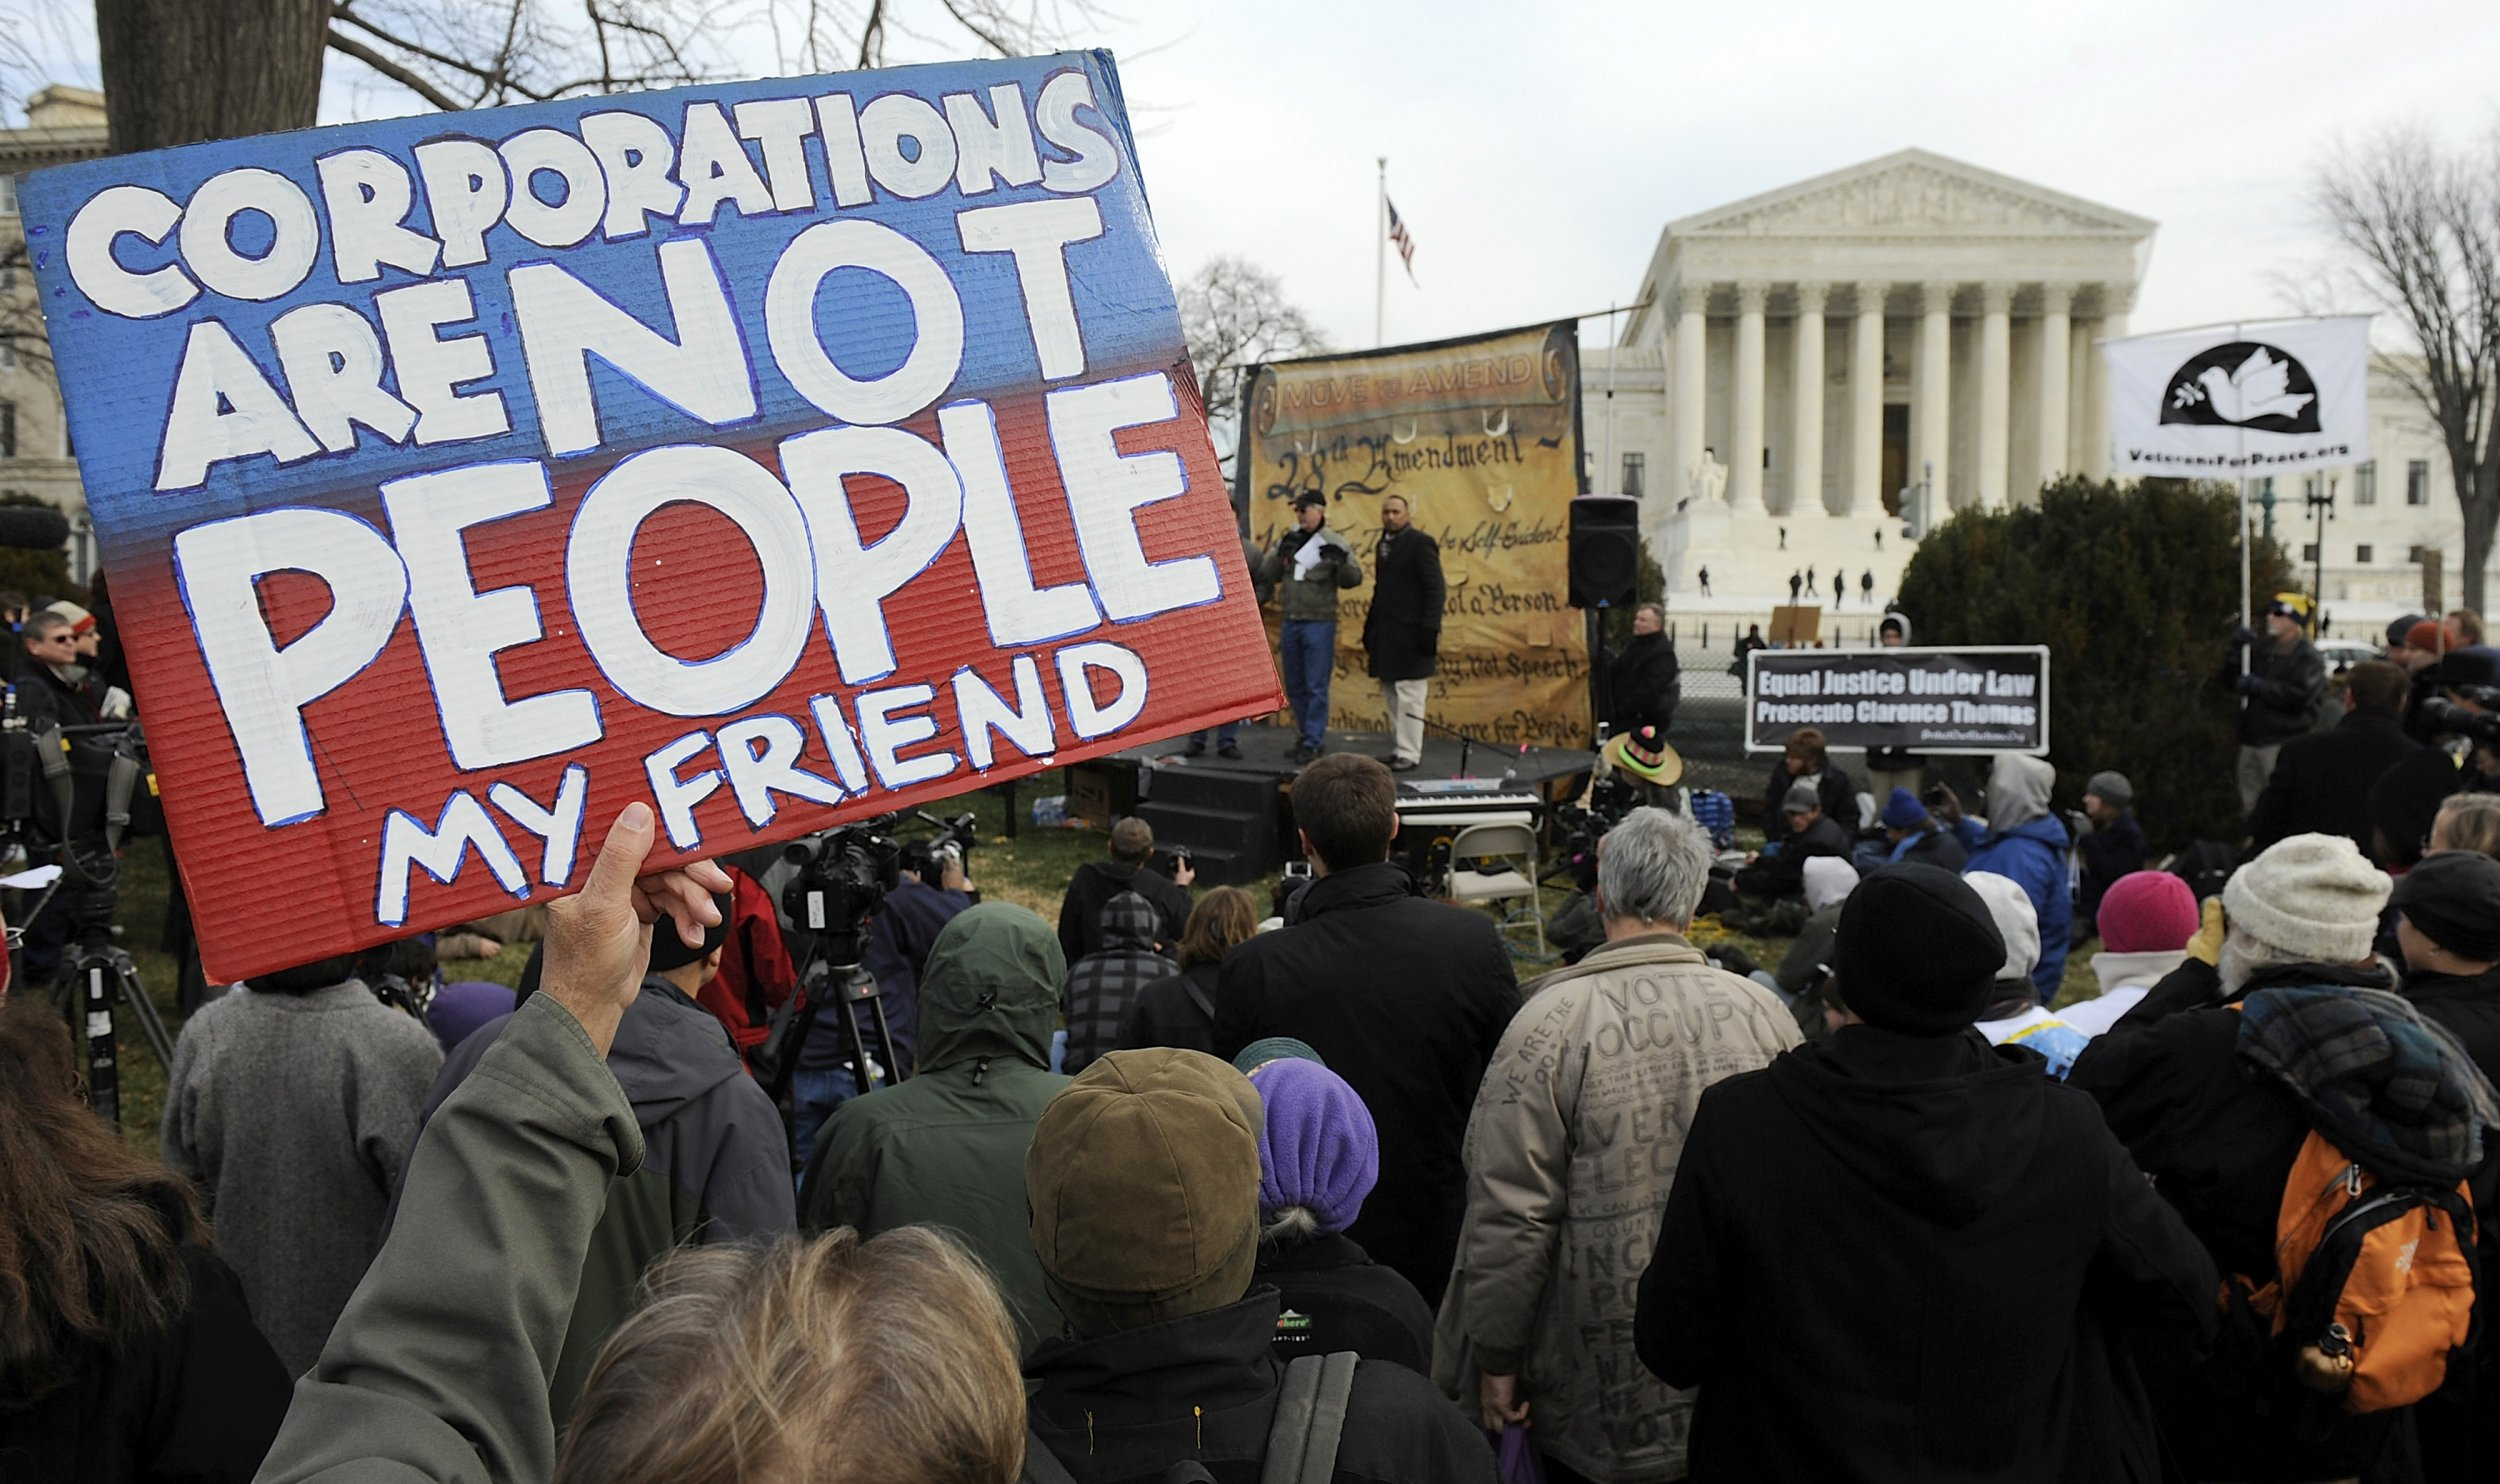
\includegraphics[max width=0.95\textwidth,
        max height=0.48000\textheight]{{Images/citizens-united-decision}.jpg}
    \end{center}
    \end{column}
    \end{columns}
}
\end{frame}
\begin{frame}[t]{Round 3 --- Famous Court Cases --- \mbox{Answer 4}}
\vspace{-0.5em}
\begin{block}{Question}
The Supreme Court's action in which case halted the recount in the 2000 presidential election?
\end{block}

\visible<2->{
    \begin{columns}[T,totalwidth=\linewidth]
    \begin{column}{0.32\linewidth}
    \begin{block}{Answer}
    Bush v. Gore (2000)
    \end{block}
    \end{column}
    \begin{column}{0.65\linewidth}
    \begin{center}
    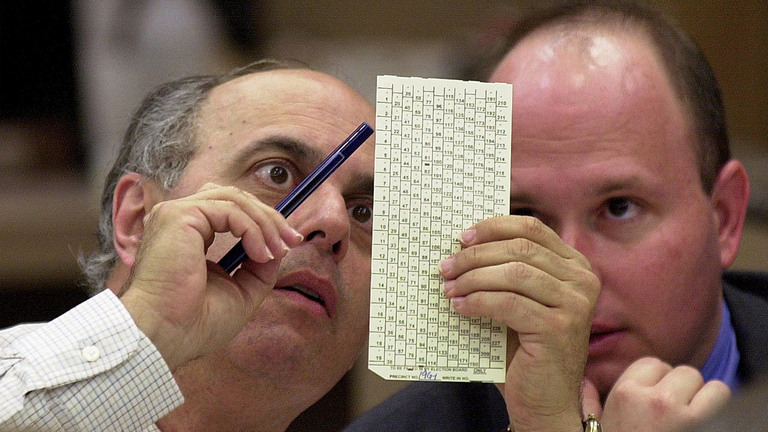
\includegraphics[max width=0.95\textwidth,
        max height=0.53000\textheight]{{Images/hanging-chad}.jpg}
    \end{center}
    \end{column}
    \end{columns}
}
\end{frame}
\begin{frame}[t]{Round 3 --- Famous Court Cases --- \mbox{Answer 5}}
\vspace{-0.5em}
\begin{block}{Question}
What court case about teaching evolution was known as the ``Monkey Trial?''
\end{block}

\visible<2->{
    \begin{columns}[T,totalwidth=\linewidth]
    \begin{column}{0.32\linewidth}
    \begin{block}{Answer}
    The State of Tennessee v. John Thomas Scopes / The Scopes Trial (1925)
    \end{block}
    \end{column}
    \begin{column}{0.65\linewidth}
    \begin{center}
    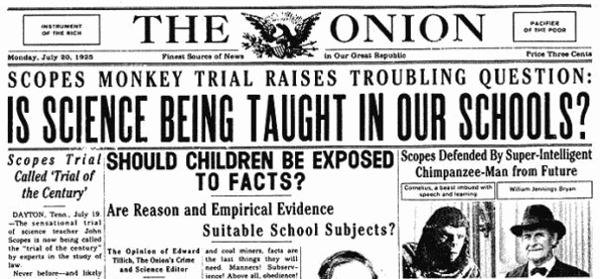
\includegraphics[max width=0.95\textwidth,
        max height=0.53000\textheight]{{Images/Onion-Scopes-small}.jpg}
    \end{center}
    \end{column}
    \end{columns}
}
\end{frame}
\begin{frame}[t]{Round 3 --- Famous Court Cases --- \mbox{Answer 6}}
\vspace{-0.5em}
\begin{block}{Question}
What two newspapers were involved in the 1971 Pentagon Papers prior restraint case?
\end{block}

\visible<2->{
    \begin{columns}[T,totalwidth=\linewidth]
    \begin{column}{0.32\linewidth}
    \begin{block}{Answer}
    The New York Times and The Washington Post
    \end{block}
    \end{column}
    \begin{column}{0.65\linewidth}
    \begin{center}
    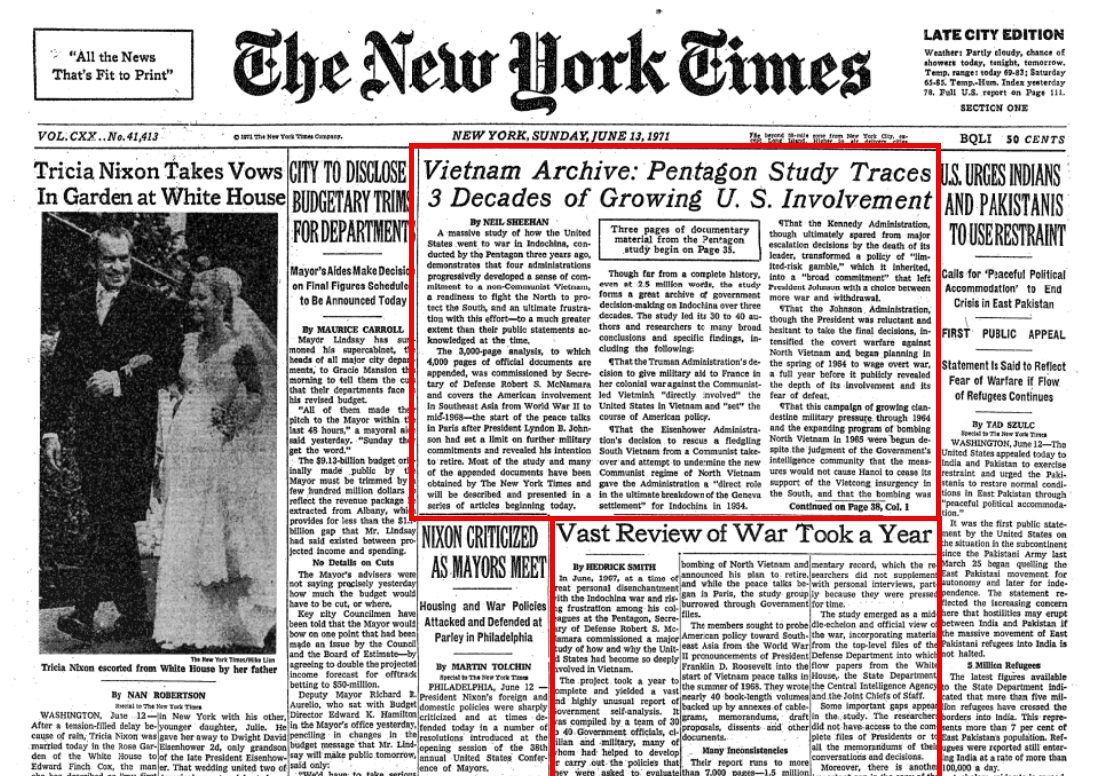
\includegraphics[max width=0.95\textwidth,
        max height=0.53000\textheight]{{Images/pentagon-papers}.jpg}
    \end{center}
    \end{column}
    \end{columns}
}
\end{frame}
\begin{frame}[t]{Round 3 --- Famous Court Cases --- \mbox{Answer 7}}
\vspace{-0.5em}
\begin{block}{Question}
In his dissent in  Schenck v. United States, Justice Holmes put forth his famous example of speech that is not protected by the First Amendment.  What was his example of such speech?
\end{block}

\visible<2->{
    \begin{columns}[T,totalwidth=\linewidth]
    \begin{column}{0.32\linewidth}
    \begin{block}{Answer}
    Falsely shouting ``Fire!'' in a crowded theater.
    \end{block}
    \end{column}
    \begin{column}{0.65\linewidth}
    \begin{center}
    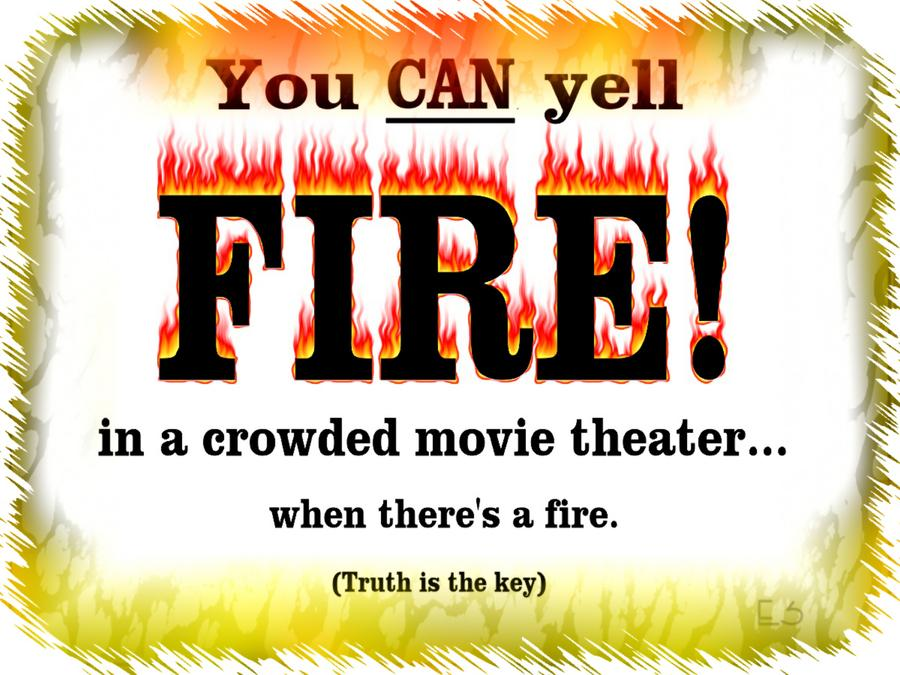
\includegraphics[max width=0.95\textwidth,
        max height=0.43000\textheight]{{Images/theater-fire}.jpg}
    \end{center}
    \end{column}
    \end{columns}
}
\end{frame}
\begin{frame}[t]{Round 3 --- Famous Court Cases --- \mbox{Answer 8}}
\vspace{-0.5em}
\begin{block}{Question}
In which case did the Supreme Court hold that when a person is arrested, he or she must be ``read their rights'' by the arresting officer?
\end{block}

\visible<2->{
    \begin{columns}[T,totalwidth=\linewidth]
    \begin{column}{0.32\linewidth}
    \begin{block}{Answer}
    Miranda v. Arizona (1966)
    \end{block}
    \end{column}
    \begin{column}{0.65\linewidth}
    \begin{center}
    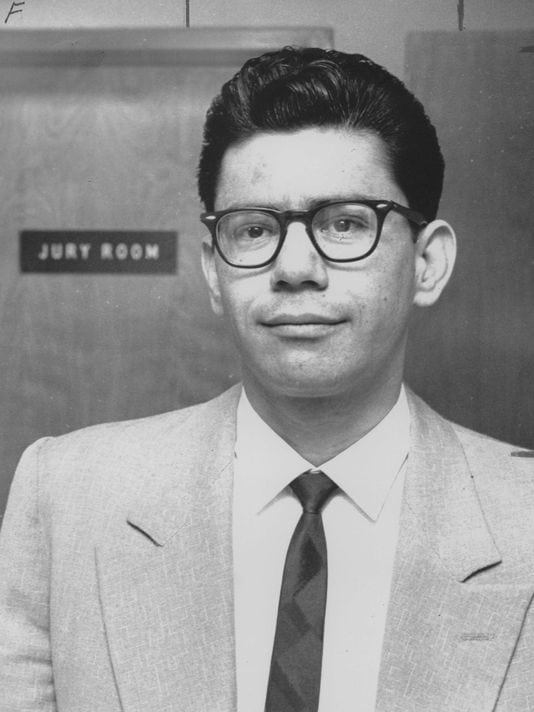
\includegraphics[max width=0.95\textwidth,
        max height=0.48000\textheight]{{Images/Miranda}.jpg}
    \end{center}
    \end{column}
    \end{columns}
}
\end{frame}
\begin{frame}[t]{Round 3 --- Famous Court Cases --- \mbox{Answer 9}}
\vspace{-0.5em}
\begin{block}{Question}
In which case did the Supreme Court hold that criminal defendants have the right to be represented by an  attorney at no cost? 
\end{block}

\visible<2->{
    \begin{columns}[T,totalwidth=\linewidth]
    \begin{column}{0.32\linewidth}
    \begin{block}{Answer}
    Gideon v. Wainwright (1963)
    \end{block}
    \end{column}
    \begin{column}{0.65\linewidth}
    \begin{center}
    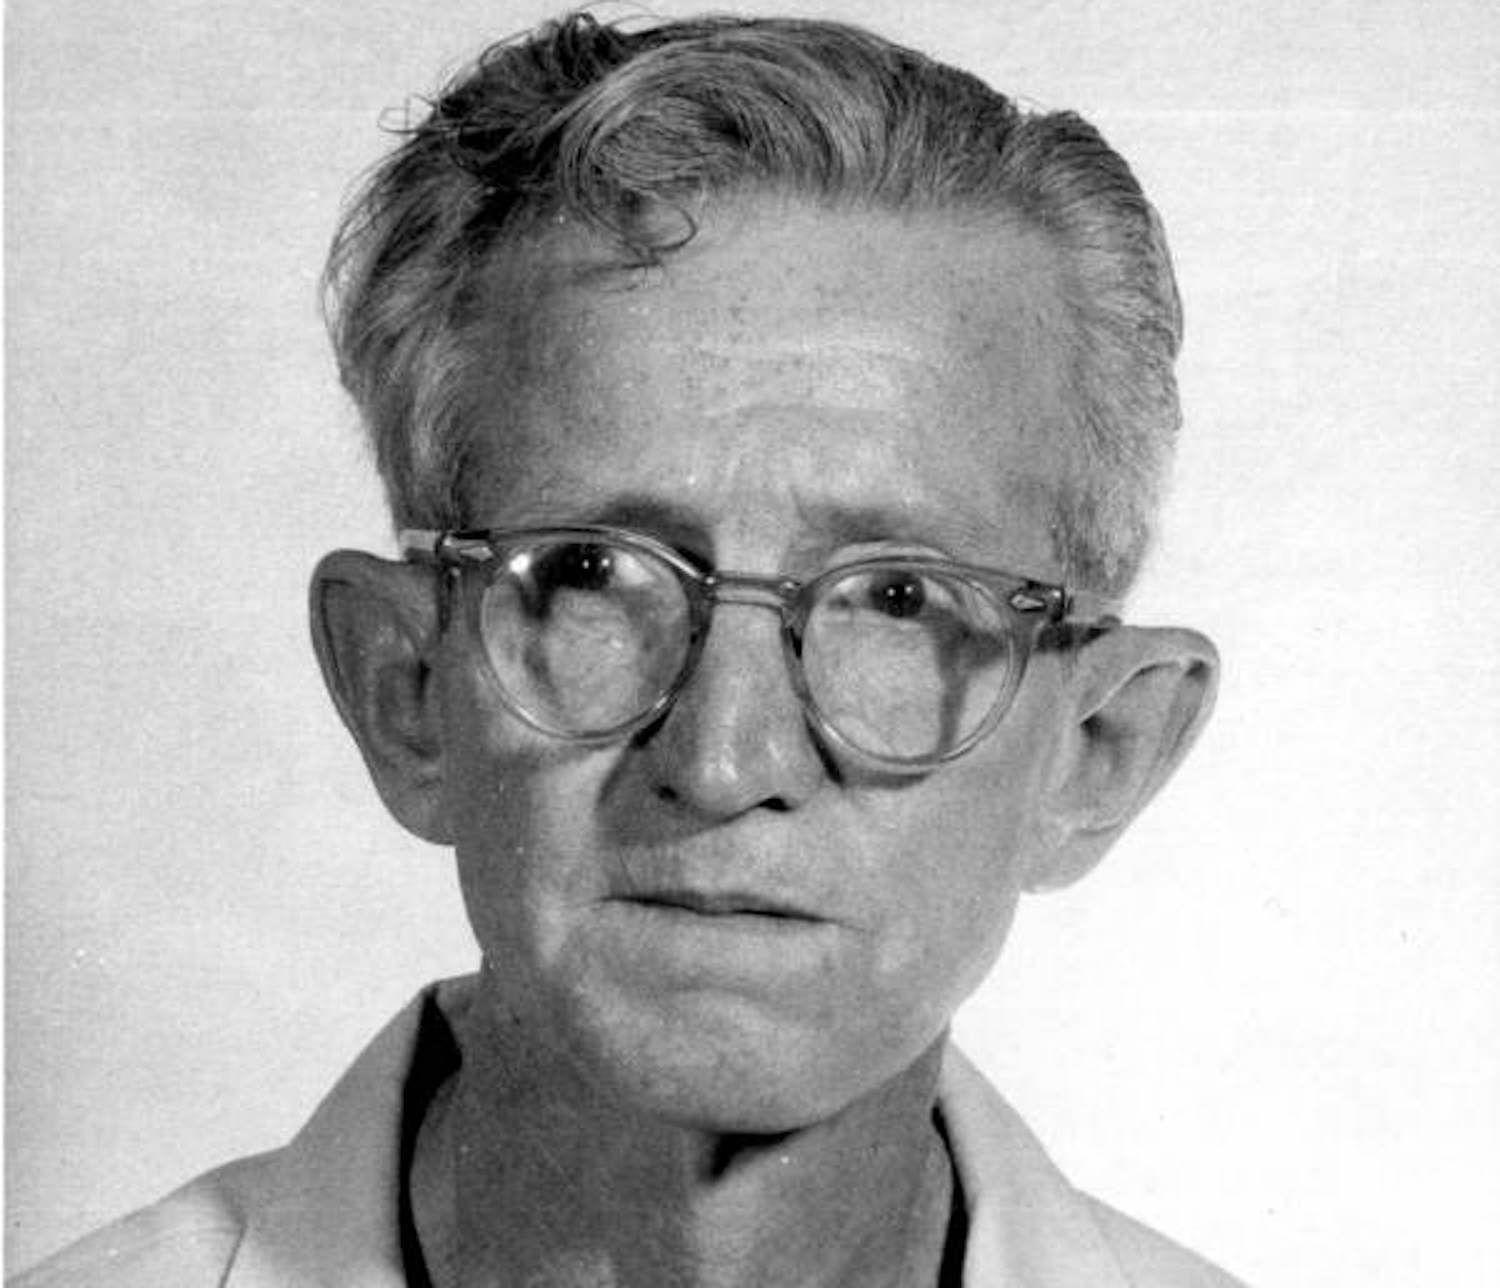
\includegraphics[max width=0.95\textwidth,
        max height=0.48000\textheight]{{Images/gideon}.jpg}
    \end{center}
    \end{column}
    \end{columns}
}
\end{frame}
\begin{frame}[t]{Round 3 --- Famous Court Cases --- \mbox{Answer 10}}
\vspace{-0.5em}
\begin{block}{Question}
In which case did the Supreme Court render its infamous decision upholding the government's internment of Americans of Japanese ancestry during World War II\@?
\end{block}

\visible<2->{
    \begin{columns}[T,totalwidth=\linewidth]
    \begin{column}{0.32\linewidth}
    \begin{block}{Answer}
    Korematsu v. United States (1944)
    \end{block}
    \end{column}
    \begin{column}{0.65\linewidth}
    \begin{center}
    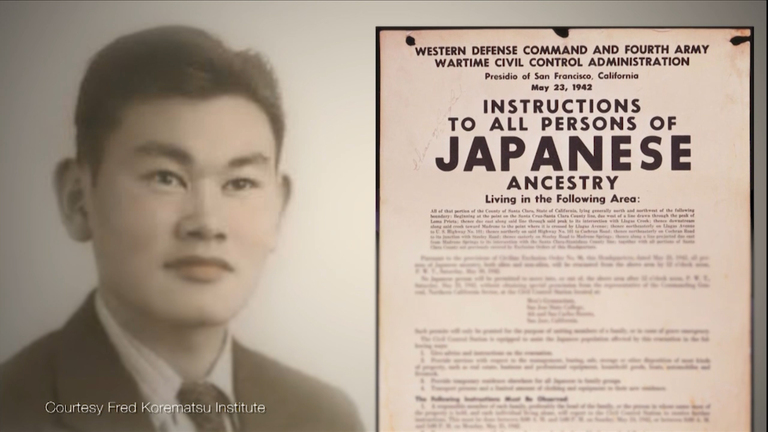
\includegraphics[max width=0.95\textwidth,
        max height=0.43000\textheight]{{Images/korematsu}.jpg}
    \end{center}
    \end{column}
    \end{columns}
}
\end{frame}
\def\thisSectionName{Biden/Harris}
\section{Round 4}
\subsection*{Q1}
\begin{frame}[t]{Round 4 --- Biden/Harris --- \mbox{Question 1}}
\vspace{-0.5em}
\begin{block}{Question}
In what year was Joe Biden born?
\end{block}
\end{frame}
\subsection*{Q2}
\begin{frame}[t]{Round 4 --- Biden/Harris --- \mbox{Question 2}}
\vspace{-0.5em}
\begin{block}{Question}
In what city was Joe Biden born?
\end{block}
\end{frame}
\subsection*{Q3}
\begin{frame}[t]{Round 4 --- Biden/Harris --- \mbox{Question 3}}
\vspace{-0.5em}
\begin{block}{Question}
In what city was Kamala Harris born?
\end{block}
\end{frame}
\subsection*{Q4}
\begin{frame}[t]{Round 4 --- Biden/Harris --- \mbox{Question 4}}
\vspace{-0.5em}
\begin{block}{Question}
Fill in the blank in Joe Biden's favorite phrase: ``Now here's the \textunderscore{}\textunderscore{}\textunderscore{}\textunderscore{}\textunderscore{}\textunderscore{}\textunderscore{}\textunderscore{}, folks.''
\end{block}
\end{frame}
\subsection*{Q5}
\begin{frame}[t]{Round 4 --- Biden/Harris --- \mbox{Question 5}}
\vspace{-0.5em}
\begin{block}{Question}
What is Joe Biden's middle name?
\end{block}
\end{frame}
\subsection*{Q6}
\begin{frame}[t]{Round 4 --- Biden/Harris --- \mbox{Question 6}}
\vspace{-0.5em}
\begin{block}{Question}
What is Kamala Harris's middle name?
\end{block}
\end{frame}
\subsection*{Q7}
\begin{frame}[t]{Round 4 --- Biden/Harris --- \mbox{Question 7}}
\vspace{-0.5em}
\begin{block}{Question}
What statewide elected office in California did Kamala Harris hold before becoming a U.S. Senator?
\end{block}
\end{frame}
\subsection*{Q8}
\begin{frame}[t]{Round 4 --- Biden/Harris --- \mbox{Question 8}}
\vspace{-0.5em}
\begin{block}{Question}
How old was Joe Biden when he first became a U.S. Senator?
\end{block}
\end{frame}
\subsection*{Q9}
\begin{frame}[t]{Round 4 --- Biden/Harris --- \mbox{Question 9}}
\vspace{-0.5em}
\begin{block}{Question}
Where did Joe Biden go to law school?
\end{block}
\end{frame}
\subsection*{Q10}
\begin{frame}[t]{Round 4 --- Biden/Harris --- \mbox{Question 10}}
\vspace{-0.5em}
\begin{block}{Question}
Where did Kamala Harris go to law school?
\end{block}
\end{frame}
\subsection{Answers}
\begin{frame}[t]{Round 4 --- Biden/Harris --- \mbox{Answer 1}}
\vspace{-0.5em}
\begin{block}{Question}
In what year was Joe Biden born?
\end{block}

\visible<2->{
    \begin{columns}[T,totalwidth=\linewidth]
    \begin{column}{0.32\linewidth}
    \begin{block}{Answer}
    1942
    \end{block}
    \end{column}
    \begin{column}{0.65\linewidth}
    \begin{center}
    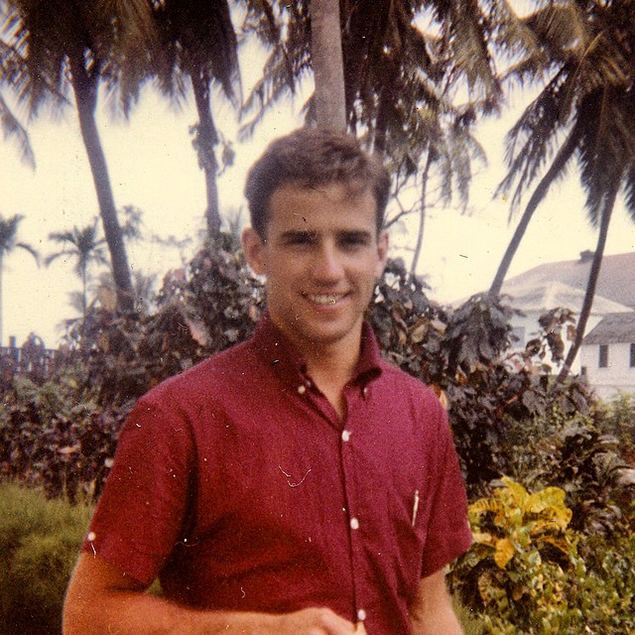
\includegraphics[max width=0.95\textwidth,
        max height=0.58000\textheight]{{Images/bidenyoung}.jpg}
    \end{center}
    \end{column}
    \end{columns}
}
\end{frame}
\begin{frame}[t]{Round 4 --- Biden/Harris --- \mbox{Answer 2}}
\vspace{-0.5em}
\begin{block}{Question}
In what city was Joe Biden born?
\end{block}

\visible<2->{
    \begin{columns}[T,totalwidth=\linewidth]
    \begin{column}{0.32\linewidth}
    \begin{block}{Answer}
    Scranton, Pennsylvania
    \end{block}
    \end{column}
    \begin{column}{0.65\linewidth}
    \begin{center}
    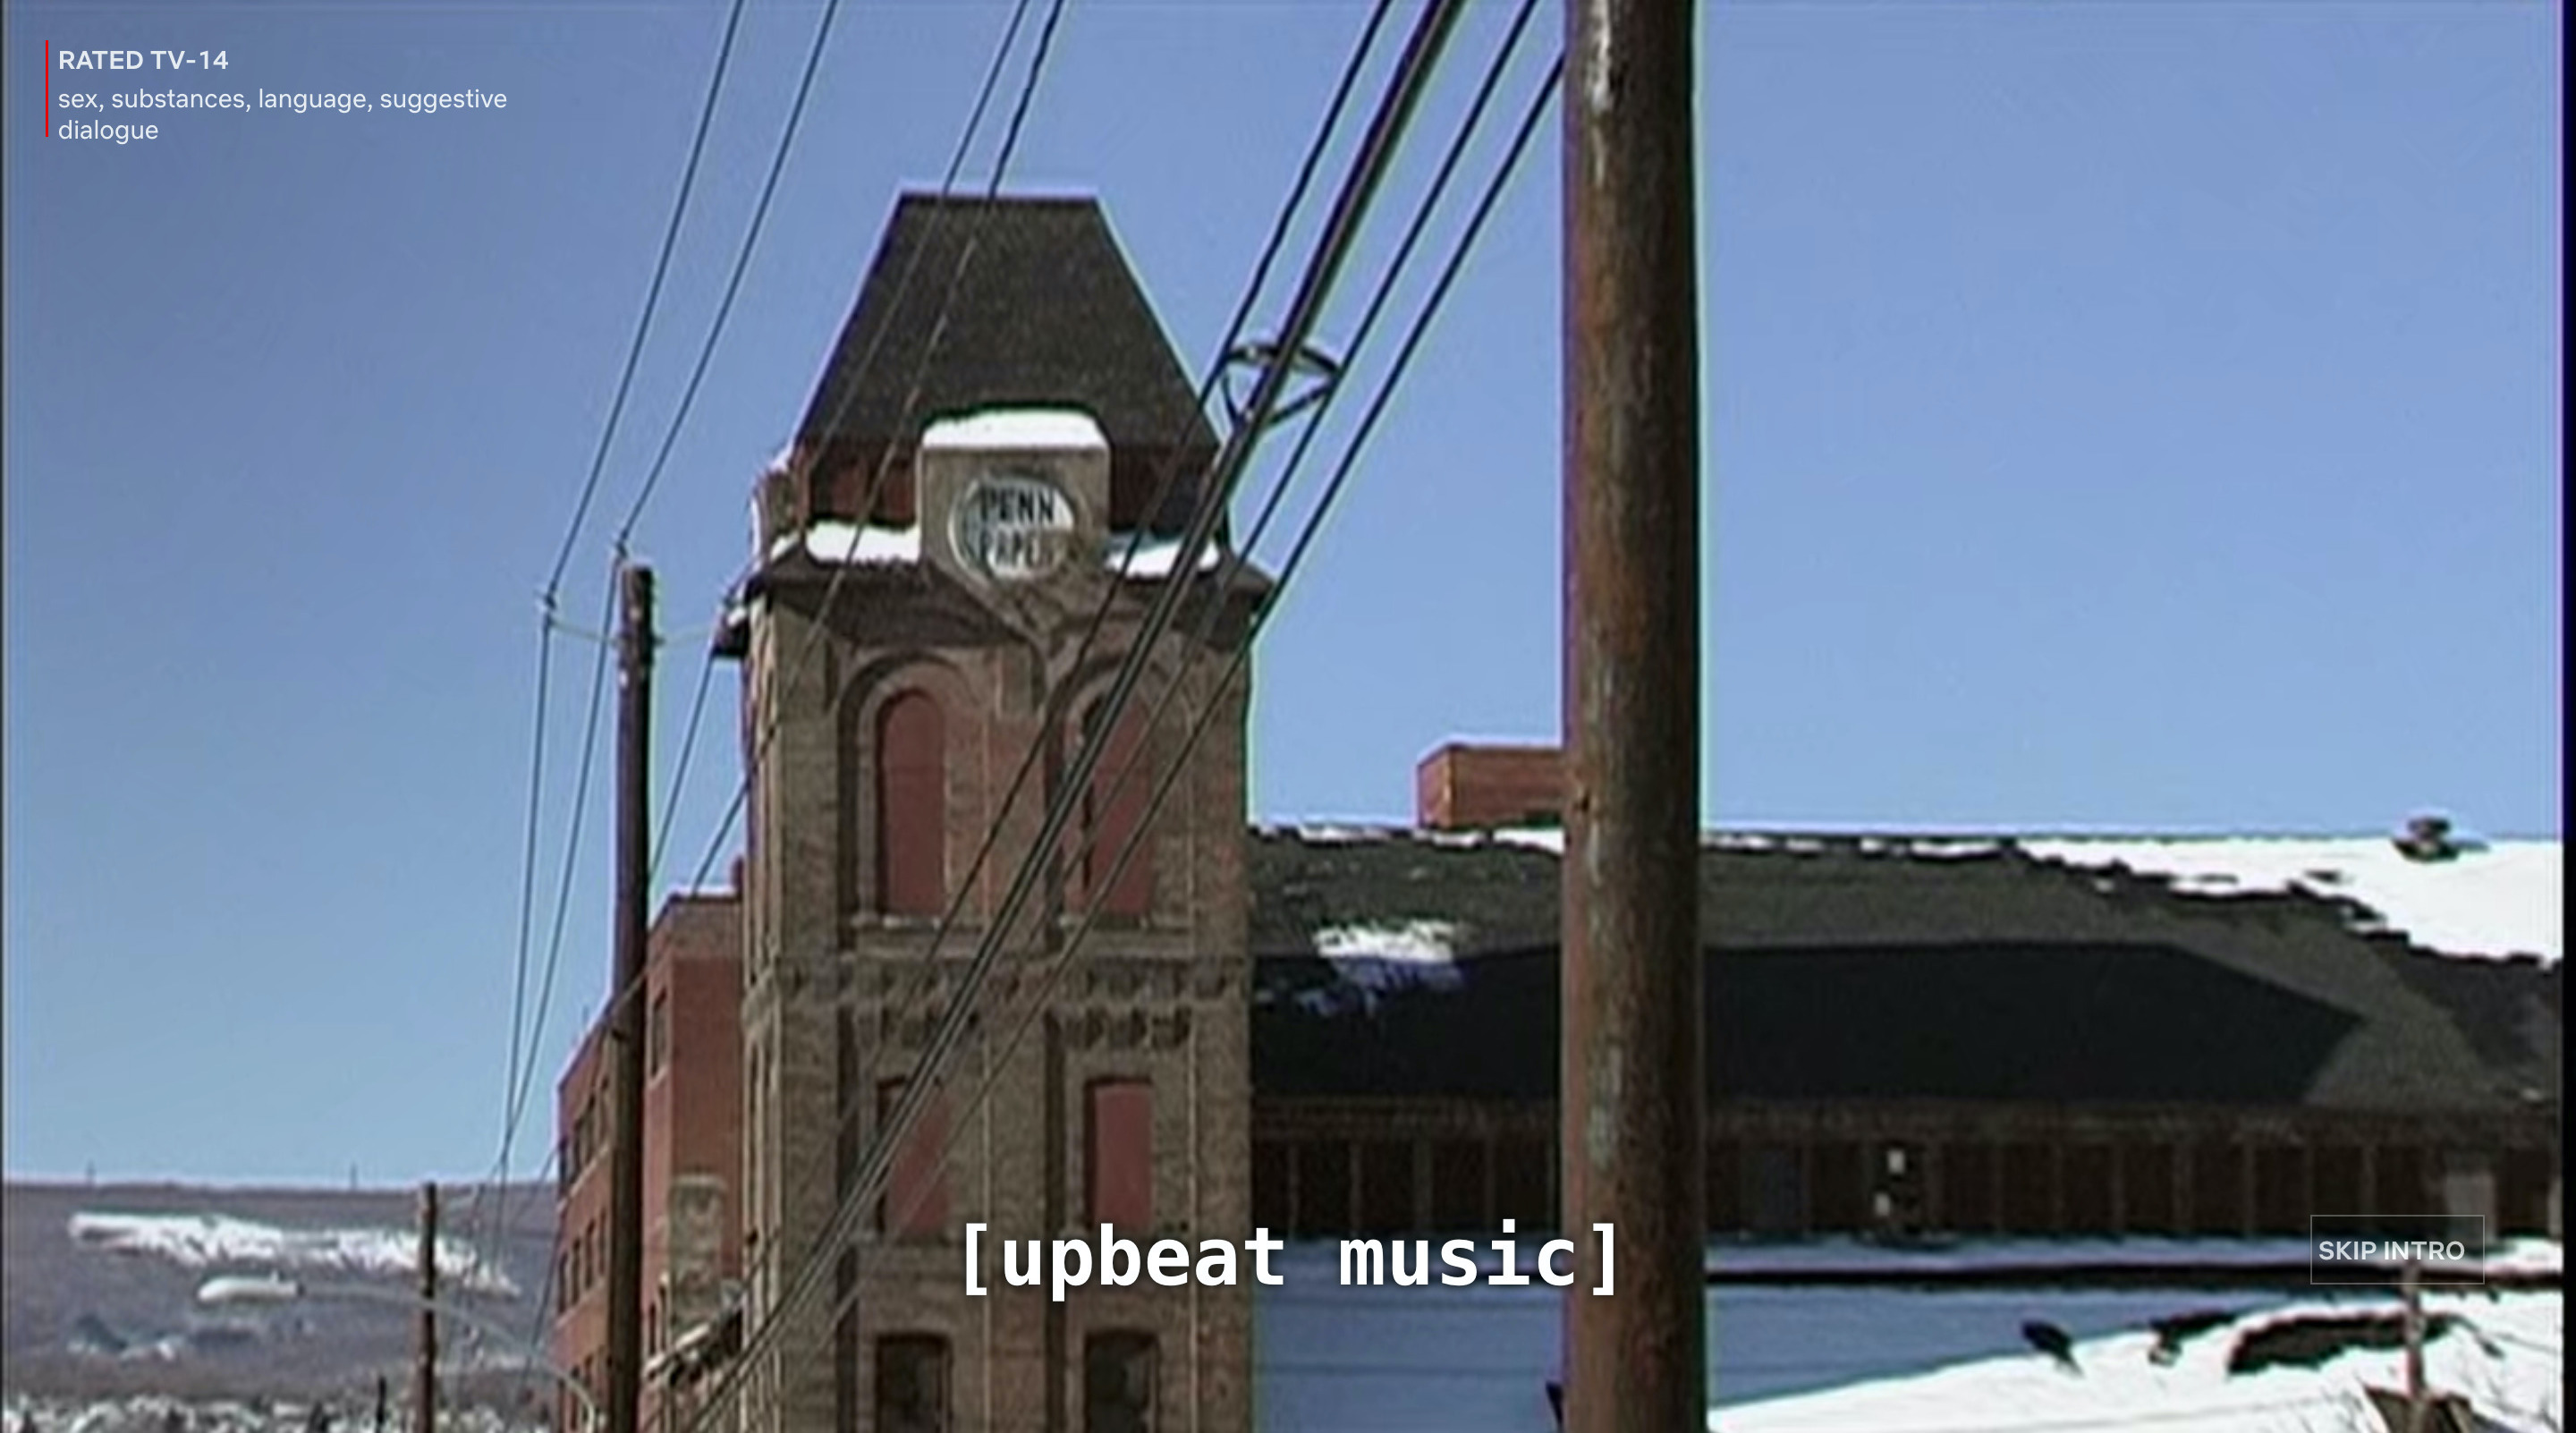
\includegraphics[max width=0.95\textwidth,
        max height=0.58000\textheight]{{Images/scranton}.jpg}
    \end{center}
    \end{column}
    \end{columns}
}
\end{frame}
\begin{frame}[t]{Round 4 --- Biden/Harris --- \mbox{Answer 3}}
\vspace{-0.5em}
\begin{block}{Question}
In what city was Kamala Harris born?
\end{block}

\visible<2->{
    \begin{columns}[T,totalwidth=\linewidth]
    \begin{column}{0.32\linewidth}
    \begin{block}{Answer}
    Oakland, California
    \end{block}
    \end{column}
    \begin{column}{0.65\linewidth}
    \begin{center}
    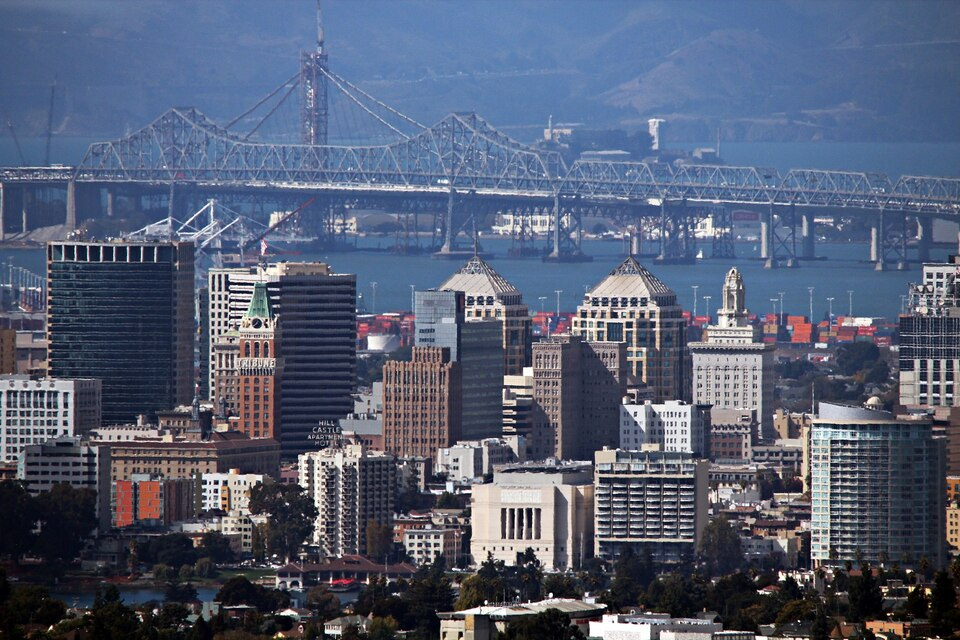
\includegraphics[max width=0.95\textwidth,
        max height=0.58000\textheight]{{Images/oakland}.JPG}
    \end{center}
    \end{column}
    \end{columns}
}
\end{frame}
\begin{frame}[t]{Round 4 --- Biden/Harris --- \mbox{Answer 4}}
\vspace{-0.5em}
\begin{block}{Question}
Fill in the blank in Joe Biden's favorite phrase: ``Now here's the \textunderscore{}\textunderscore{}\textunderscore{}\textunderscore{}\textunderscore{}\textunderscore{}\textunderscore{}\textunderscore{}, folks.''
\end{block}

\visible<2->{
    \begin{columns}[T,totalwidth=\linewidth]
    \begin{column}{0.32\linewidth}
    \begin{block}{Answer}
    Deal
    \end{block}
    \end{column}
    \begin{column}{0.65\linewidth}
    \begin{center}
    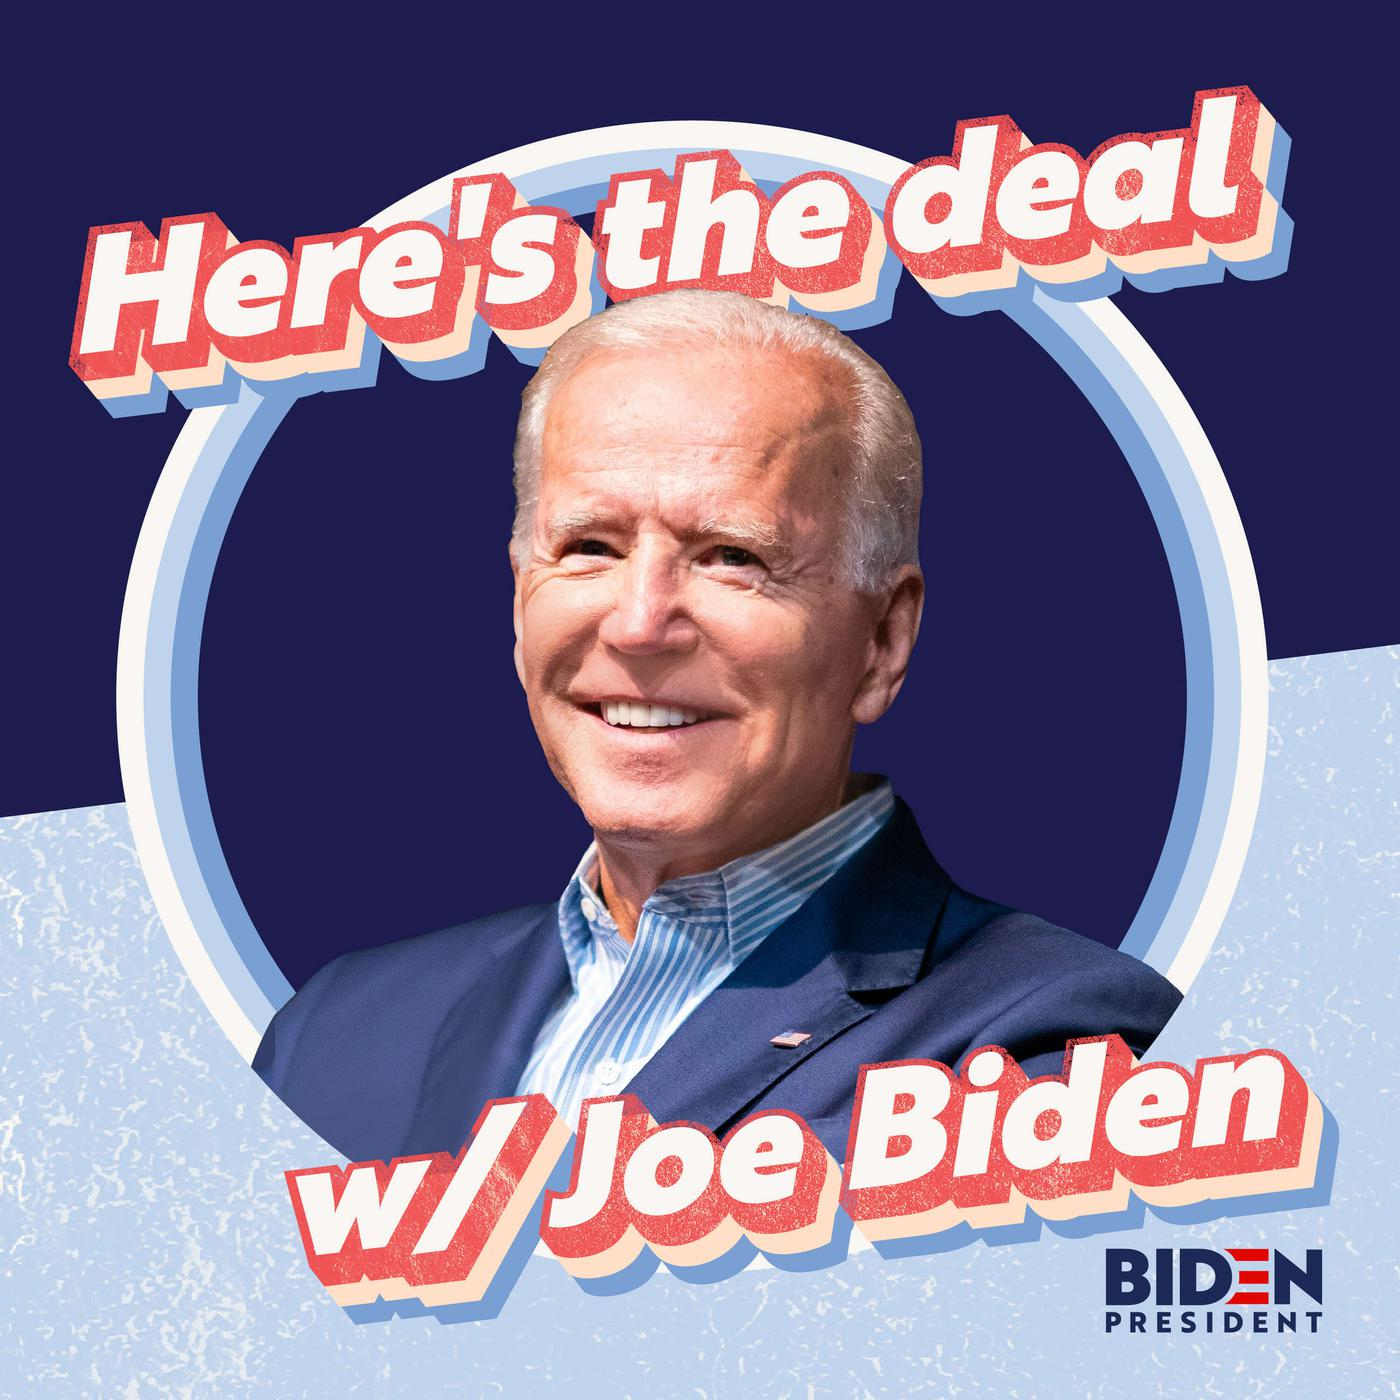
\includegraphics[max width=0.95\textwidth,
        max height=0.38000\textheight]{{Images/deal}.jpg}
    \end{center}
    \end{column}
    \end{columns}
}
\end{frame}
\begin{frame}[t]{Round 4 --- Biden/Harris --- \mbox{Answer 5}}
\vspace{-0.5em}
\begin{block}{Question}
What is Joe Biden's middle name?
\end{block}

\visible<2->{
    \begin{columns}[T,totalwidth=\linewidth]
    \begin{column}{0.32\linewidth}
    \begin{block}{Answer}
    Robinette
    \end{block}
    \end{column}
    \begin{column}{0.65\linewidth}
    \begin{center}
    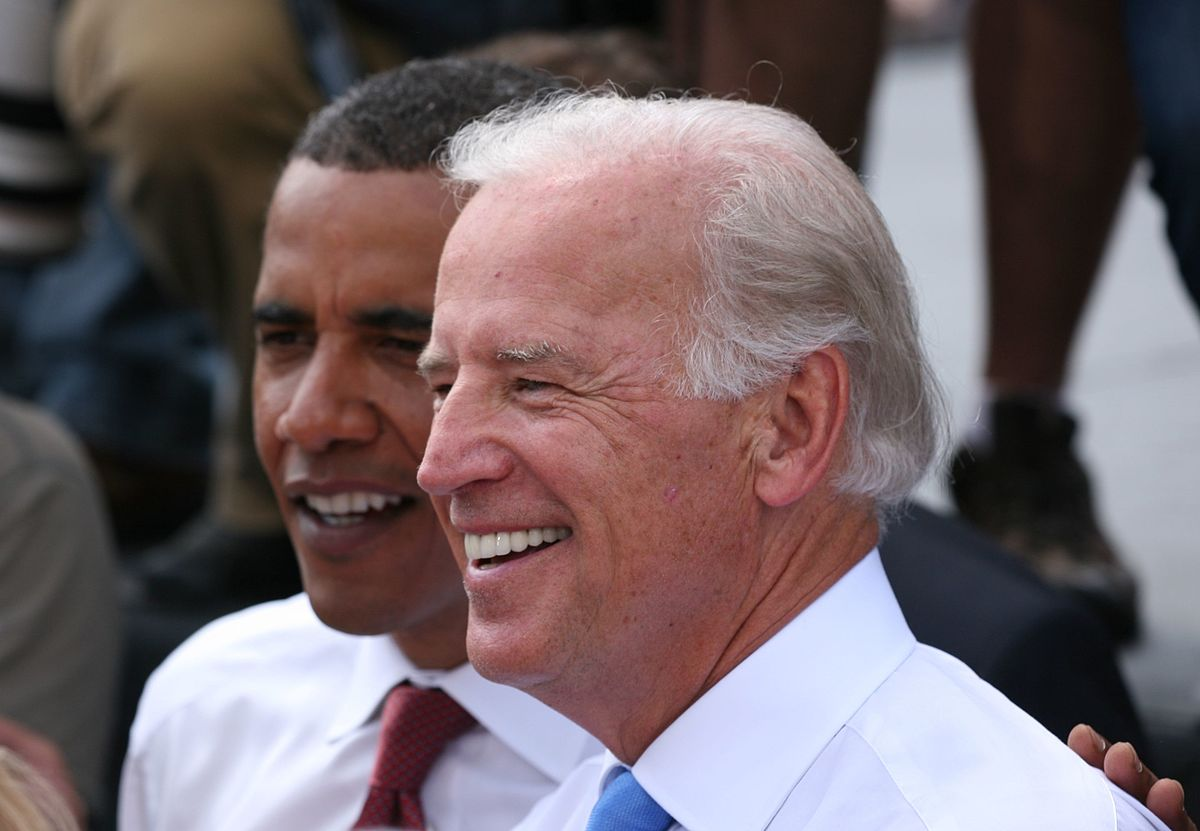
\includegraphics[max width=0.95\textwidth,
        max height=0.58000\textheight]{{Images/biden}.jpg}
    \end{center}
    \end{column}
    \end{columns}
}
\end{frame}
\begin{frame}[t]{Round 4 --- Biden/Harris --- \mbox{Answer 6}}
\vspace{-0.5em}
\begin{block}{Question}
What is Kamala Harris's middle name?
\end{block}

\visible<2->{
    \begin{columns}[T,totalwidth=\linewidth]
    \begin{column}{0.32\linewidth}
    \begin{block}{Answer}
    Devi
    \end{block}
    \end{column}
    \begin{column}{0.65\linewidth}
    \begin{center}
    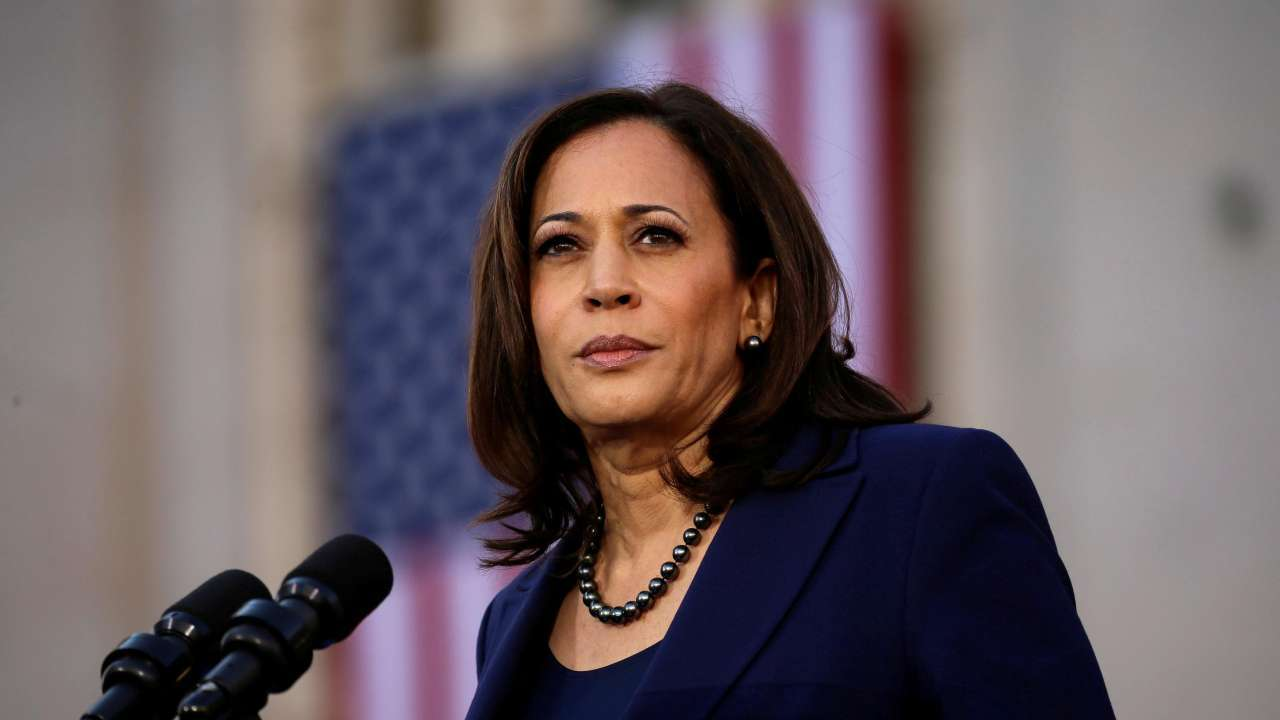
\includegraphics[max width=0.95\textwidth,
        max height=0.58000\textheight]{{Images/kamala}.jpg}
    \end{center}
    \end{column}
    \end{columns}
}
\end{frame}
\begin{frame}[t]{Round 4 --- Biden/Harris --- \mbox{Answer 7}}
\vspace{-0.5em}
\begin{block}{Question}
What statewide elected office in California did Kamala Harris hold before becoming a U.S. Senator?
\end{block}

\visible<2->{
    \begin{columns}[T,totalwidth=\linewidth]
    \begin{column}{0.32\linewidth}
    \begin{block}{Answer}
    Attorney General
    \end{block}
    \end{column}
    \begin{column}{0.65\linewidth}
    \begin{center}
    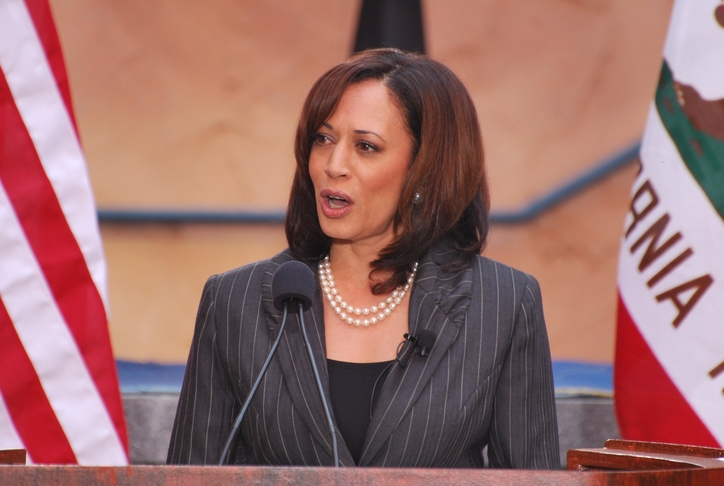
\includegraphics[max width=0.95\textwidth,
        max height=0.53000\textheight]{{Images/kamalaharrisag}.jpg}
    \end{center}
    \end{column}
    \end{columns}
}
\end{frame}
\begin{frame}[t]{Round 4 --- Biden/Harris --- \mbox{Answer 8}}
\vspace{-0.5em}
\begin{block}{Question}
How old was Joe Biden when he first became a U.S. Senator?
\end{block}

\visible<2->{
    \begin{columns}[T,totalwidth=\linewidth]
    \begin{column}{0.32\linewidth}
    \begin{block}{Answer}
    29
    \end{block}
    \end{column}
    \begin{column}{0.65\linewidth}
    \begin{center}
    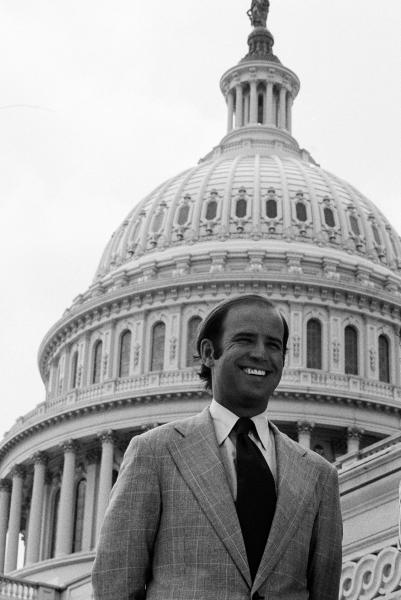
\includegraphics[max width=0.95\textwidth,
        max height=0.53000\textheight]{{Images/bidensenate}.jpg}
    \end{center}
    \end{column}
    \end{columns}
}
\end{frame}
\begin{frame}[t]{Round 4 --- Biden/Harris --- \mbox{Answer 9}}
\vspace{-0.5em}
\begin{block}{Question}
Where did Joe Biden go to law school?
\end{block}

\visible<2->{
    \begin{columns}[T,totalwidth=\linewidth]
    \begin{column}{0.32\linewidth}
    \begin{block}{Answer}
    Syracuse University
    \end{block}
    \end{column}
    \begin{column}{0.65\linewidth}
    \begin{center}
    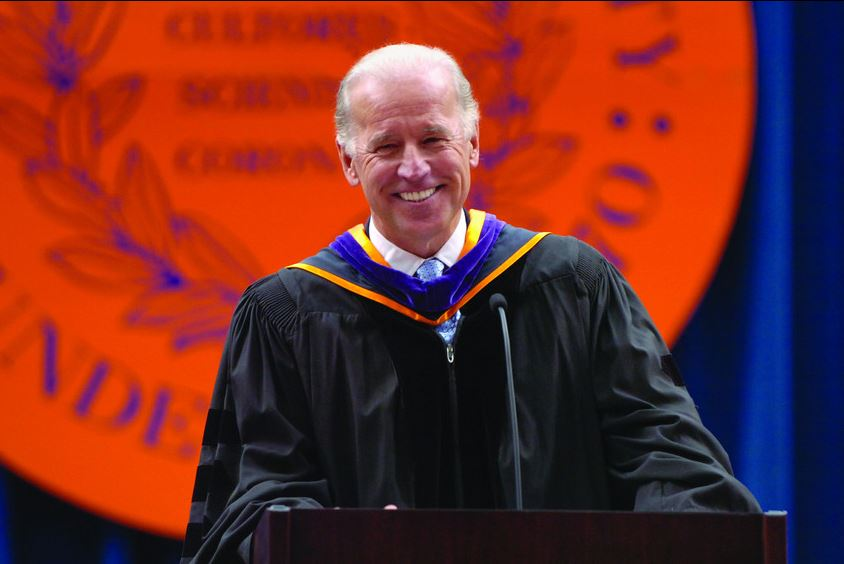
\includegraphics[max width=0.95\textwidth,
        max height=0.58000\textheight]{{Images/syracuse}.jpg}
    \end{center}
    \end{column}
    \end{columns}
}
\end{frame}
\begin{frame}[t]{Round 4 --- Biden/Harris --- \mbox{Answer 10}}
\vspace{-0.5em}
\begin{block}{Question}
Where did Kamala Harris go to law school?
\end{block}

\visible<2->{
    \begin{columns}[T,totalwidth=\linewidth]
    \begin{column}{0.32\linewidth}
    \begin{block}{Answer}
    University of California, Hastings
    \end{block}
    \end{column}
    \begin{column}{0.65\linewidth}
    \begin{center}
    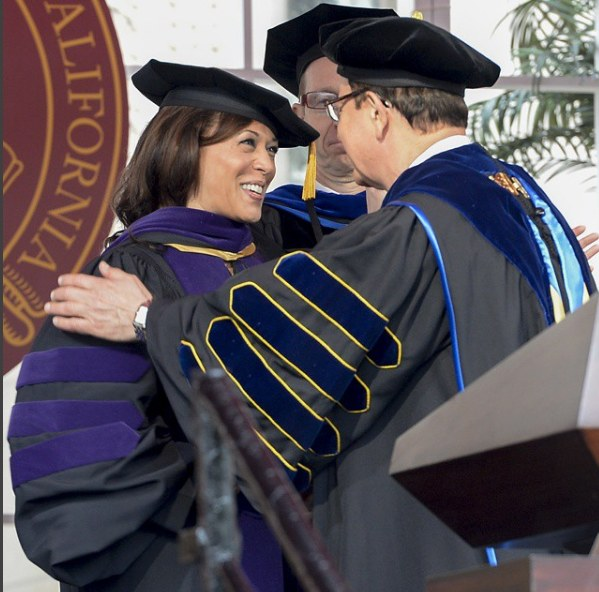
\includegraphics[max width=0.95\textwidth,
        max height=0.58000\textheight]{{Images/hastings}.jpg}
    \end{center}
    \end{column}
    \end{columns}
}
\end{frame}
\def\thisSectionName{The Holiday Season}
\section{Round 5}
\subsection*{Q1}
\begin{frame}[t]{Round 5 --- The Holiday Season --- \mbox{Question 1}}
\vspace{-0.5em}
\begin{block}{Question}
How many days long was the first Thanksgiving?
\end{block}
\end{frame}
\subsection*{Q2}
\begin{frame}[t]{Round 5 --- The Holiday Season --- \mbox{Question 2}}
\vspace{-0.5em}
\begin{block}{Question}
After Black Friday, which day is typically the biggest shopping day of the holiday season? (Some years, it even surpasses Black Friday.)
\end{block}
\end{frame}
\subsection*{Q3}
\begin{frame}[t]{Round 5 --- The Holiday Season --- \mbox{Question 3}}
\vspace{-0.5em}
\begin{block}{Question}
From which Ancient Roman winter holiday are many of the customs associated with Christmas thought to have been derived?
\end{block}
\end{frame}
\subsection*{Q4}
\begin{frame}[t]{Round 5 --- The Holiday Season --- \mbox{Question 4}}
\vspace{-0.5em}
\begin{block}{Question}
Who wrote the musical score for \emph{A Charlie Brown Christmas}?
\end{block}
\end{frame}
\subsection*{Q5}
\begin{frame}[t]{Round 5 --- The Holiday Season --- \mbox{Question 5}}
\vspace{-0.5em}
\begin{block}{Question}
According to Spanish tradition, how many grapes should you eat at the stroke of midnight on New Year's Eve?
\end{block}
\end{frame}
\subsection*{Q6}
\begin{frame}[t]{Round 5 --- The Holiday Season --- \mbox{Question 6}}
\vspace{-0.5em}
\begin{block}{Question}
According to \emph{The Village Voice}, which annual holiday-season event began as ``joyful performance art'', but has since evolved into a ``reviled bar crawl''?
\end{block}
\end{frame}
\subsection*{Q7}
\begin{frame}[t]{Round 5 --- The Holiday Season --- \mbox{Question 7}}
\vspace{-0.5em}
\begin{block}{Question}
On what dates does Kwanzaa begin and end?
\end{block}
\end{frame}
\subsection*{Q8}
\begin{frame}[t]{Round 5 --- The Holiday Season --- \mbox{Question 8}}
\vspace{-0.5em}
\begin{block}{Question}
What was the original title of the poem often referred to by its first line, \emph{`Twas the night before Christmas}? 
\end{block}
\end{frame}
\subsection*{Q9}
\begin{frame}[t]{Round 5 --- The Holiday Season --- \mbox{Question 9}}
\vspace{-0.5em}
\begin{block}{Question}
Without using a calculator, how many candles are used by a menorah over the course of Chanukah? (Assume no reuse of candles.)
\end{block}
\end{frame}
\subsection*{Q10}
\begin{frame}[t]{Round 5 --- The Holiday Season --- \mbox{Question 10}}
\vspace{-0.5em}
\begin{block}{Question}
In the song ``The Twelve Days of Christmas'', what gift was given on the twelfth and final day?
\end{block}
\end{frame}
\subsection{Answers}
\begin{frame}[t]{Round 5 --- The Holiday Season --- \mbox{Answer 1}}
\vspace{-0.5em}
\begin{block}{Question}
How many days long was the first Thanksgiving?
\end{block}

\visible<2->{
    \begin{columns}[T,totalwidth=\linewidth]
    \begin{column}{0.32\linewidth}
    \begin{block}{Answer}
    Three days
    \end{block}
    \end{column}
    \begin{column}{0.65\linewidth}
    \begin{center}
    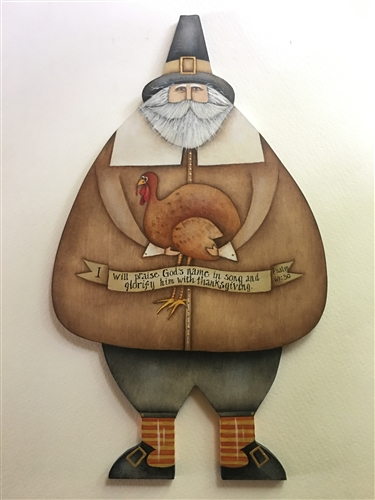
\includegraphics[max width=0.95\textwidth,
        max height=0.58000\textheight]{{Images/fatpilgrim}.jpg}
    \end{center}
    \end{column}
    \end{columns}
}
\end{frame}
\begin{frame}[t]{Round 5 --- The Holiday Season --- \mbox{Answer 2}}
\vspace{-0.5em}
\begin{block}{Question}
After Black Friday, which day is typically the biggest shopping day of the holiday season? (Some years, it even surpasses Black Friday.)
\end{block}

\visible<2->{
    \begin{columns}[T,totalwidth=\linewidth]
    \begin{column}{0.32\linewidth}
    \begin{block}{Answer}
    Super Saturday / Panic Saturday / The Saturday before Christmas
    \end{block}
    \end{column}
    \begin{column}{0.65\linewidth}
    \begin{center}
    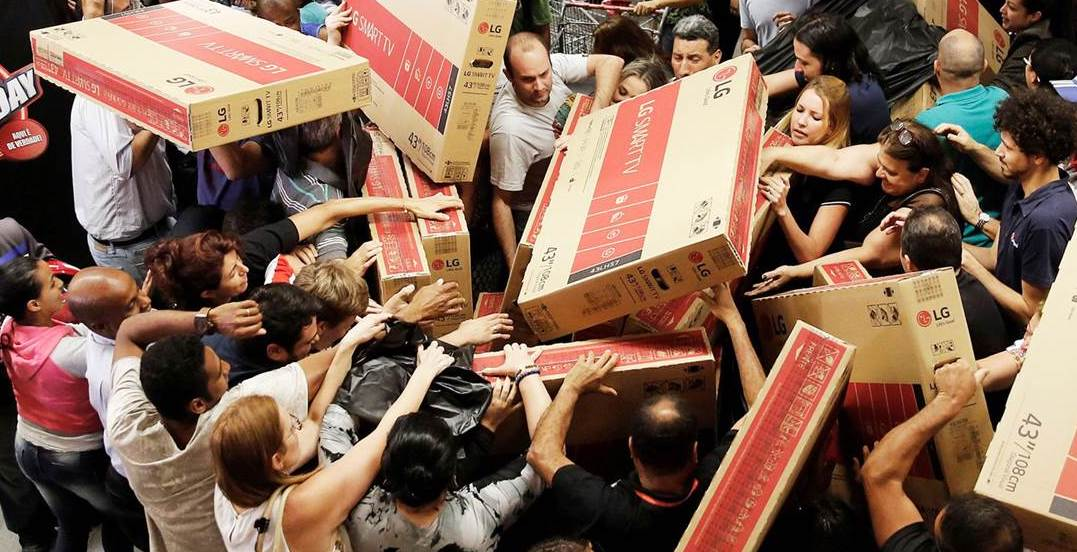
\includegraphics[max width=0.95\textwidth,
        max height=0.48000\textheight]{{Images/supersaturday}.jpg}
    \end{center}
    \end{column}
    \end{columns}
}
\end{frame}
\begin{frame}[t]{Round 5 --- The Holiday Season --- \mbox{Answer 3}}
\vspace{-0.5em}
\begin{block}{Question}
From which Ancient Roman winter holiday are many of the customs associated with Christmas thought to have been derived?
\end{block}

\visible<2->{
    \begin{columns}[T,totalwidth=\linewidth]
    \begin{column}{0.32\linewidth}
    \begin{block}{Answer}
    Saturnalia
    \end{block}
    \end{column}
    \begin{column}{0.65\linewidth}
    \begin{center}
    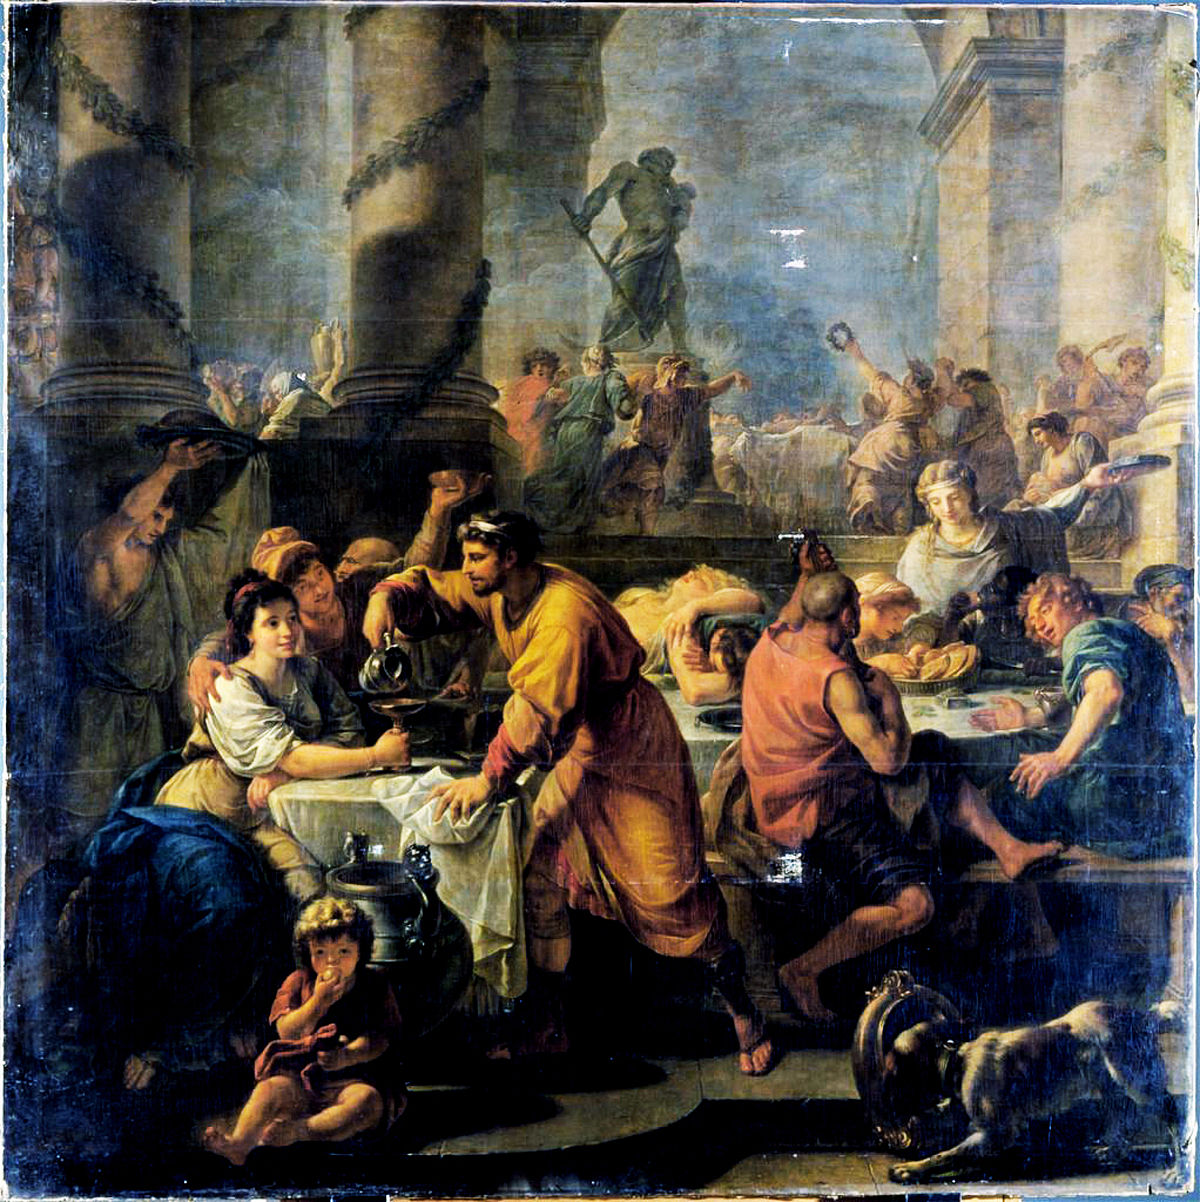
\includegraphics[max width=0.95\textwidth,
        max height=0.48000\textheight]{{Images/saturnalia}.jpg}
    \end{center}
    \end{column}
    \end{columns}
}
\end{frame}
\begin{frame}[t]{Round 5 --- The Holiday Season --- \mbox{Answer 4}}
\vspace{-0.5em}
\begin{block}{Question}
Who wrote the musical score for \emph{A Charlie Brown Christmas}?
\end{block}

\visible<2->{
    \begin{columns}[T,totalwidth=\linewidth]
    \begin{column}{0.32\linewidth}
    \begin{block}{Answer}
    Vince Guaraldi
    \end{block}
    \end{column}
    \begin{column}{0.65\linewidth}
    \begin{center}
    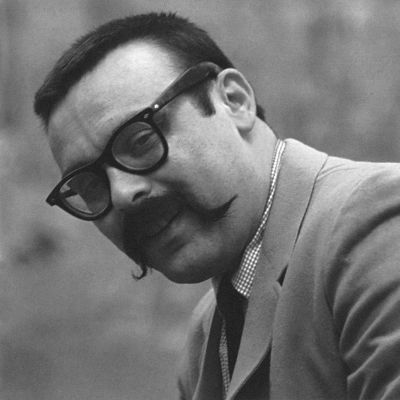
\includegraphics[max width=0.95\textwidth,
        max height=0.53000\textheight]{{Images/guaraldi}.jpg}
    \end{center}
    \end{column}
    \end{columns}
}
\end{frame}
\begin{frame}[t]{Round 5 --- The Holiday Season --- \mbox{Answer 5}}
\vspace{-0.5em}
\begin{block}{Question}
According to Spanish tradition, how many grapes should you eat at the stroke of midnight on New Year's Eve?
\end{block}

\visible<2->{
    \begin{columns}[T,totalwidth=\linewidth]
    \begin{column}{0.32\linewidth}
    \begin{block}{Answer}
    Twelve
    \end{block}
    \end{column}
    \begin{column}{0.65\linewidth}
    \begin{center}
    \includegraphics[max width=0.95\textwidth,
        max height=0.48000\textheight]{{Images/spaingrapes}.jpg}
    \end{center}
    \end{column}
    \end{columns}
}
\end{frame}
\begin{frame}[t]{Round 5 --- The Holiday Season --- \mbox{Answer 6}}
\vspace{-0.5em}
\begin{block}{Question}
According to \emph{The Village Voice}, which annual holiday-season event began as ``joyful performance art'', but has since evolved into a ``reviled bar crawl''?
\end{block}

\visible<2->{
    \begin{columns}[T,totalwidth=\linewidth]
    \begin{column}{0.32\linewidth}
    \begin{block}{Answer}
    SantaCon
    \end{block}
    \end{column}
    \begin{column}{0.65\linewidth}
    \begin{center}
    \includegraphics[max width=0.95\textwidth,
        max height=0.43000\textheight]{{Images/santacon}.jpeg}
    \end{center}
    \end{column}
    \end{columns}
}
\end{frame}
\begin{frame}[t]{Round 5 --- The Holiday Season --- \mbox{Answer 7}}
\vspace{-0.5em}
\begin{block}{Question}
On what dates does Kwanzaa begin and end?
\end{block}

\visible<2->{
    \begin{columns}[T,totalwidth=\linewidth]
    \begin{column}{0.32\linewidth}
    \begin{block}{Answer}
    December 26--January 1
    \end{block}
    \end{column}
    \begin{column}{0.65\linewidth}
    \begin{center}
    \includegraphics[max width=0.95\textwidth,
        max height=0.58000\textheight]{{Images/kwanzaa-usa}.jpg}
    \end{center}
    \end{column}
    \end{columns}
}
\end{frame}
\begin{frame}[t]{Round 5 --- The Holiday Season --- \mbox{Answer 8}}
\vspace{-0.5em}
\begin{block}{Question}
What was the original title of the poem often referred to by its first line, \emph{`Twas the night before Christmas}? 
\end{block}

\visible<2->{
    \begin{columns}[T,totalwidth=\linewidth]
    \begin{column}{0.32\linewidth}
    \begin{block}{Answer}
    \emph{A Visit from St.\ Nicholas} (by Clement Clarke Moore)
    \end{block}
    \end{column}
    \begin{column}{0.65\linewidth}
    \begin{center}
    \includegraphics[max width=0.95\textwidth,
        max height=0.48000\textheight]{{Images/stnick}.jpg}
    \end{center}
    \end{column}
    \end{columns}
}
\end{frame}
\begin{frame}[t]{Round 5 --- The Holiday Season --- \mbox{Answer 9}}
\vspace{-0.5em}
\begin{block}{Question}
Without using a calculator, how many candles are used by a menorah over the course of Chanukah? (Assume no reuse of candles.)
\end{block}

\visible<2->{
    \begin{columns}[T,totalwidth=\linewidth]
    \begin{column}{0.32\linewidth}
    \begin{block}{Answer}
    44 ($2+3+\cdots+8+9$)
    \end{block}
    \end{column}
    \begin{column}{0.65\linewidth}
    \begin{center}
    \includegraphics[max width=0.95\textwidth,
        max height=0.48000\textheight]{{Images/menorah}.jpg}
    \end{center}
    \end{column}
    \end{columns}
}
\end{frame}
\begin{frame}[t]{Round 5 --- The Holiday Season --- \mbox{Answer 10}}
\vspace{-0.5em}
\begin{block}{Question}
In the song ``The Twelve Days of Christmas'', what gift was given on the twelfth and final day?
\end{block}

\visible<2->{
    \begin{columns}[T,totalwidth=\linewidth]
    \begin{column}{0.32\linewidth}
    \begin{block}{Answer}
    Twelve drummers drumming
    \end{block}
    \end{column}
    \begin{column}{0.65\linewidth}
    \begin{center}
    \includegraphics[max width=0.95\textwidth,
        max height=0.53000\textheight]{{Images/12Days-1}.jpg}
    \end{center}
    \end{column}
    \end{columns}
}
\end{frame}
\def\thisSectionName{Scientific Breakthroughs}
\section{Round 6}
\subsection*{Q1}
\begin{frame}[t]{Round 6 --- Scientific Breakthroughs --- \mbox{Question 1}}
\vspace{-0.5em}
\begin{block}{Question}
Which scientist --- arguably history's first ``revolutionary'' scientist --- developed the first heliocentric model of the solar system?
\end{block}
\end{frame}
\subsection*{Q2}
\begin{frame}[t]{Round 6 --- Scientific Breakthroughs --- \mbox{Question 2}}
\vspace{-0.5em}
\begin{block}{Question}
When Alexander Fleming discovered that mold had destroyed his bacterial cultures, he developed the mold into what medicine?
\end{block}
\end{frame}
\subsection*{Q3}
\begin{frame}[t]{Round 6 --- Scientific Breakthroughs --- \mbox{Question 3}}
\vspace{-0.5em}
\begin{block}{Question}
Max Planck solved the ``ultraviolet catastrophe'' by positing that electromagnetic radiation only came in discrete packets that we now know by what name?
\end{block}
\end{frame}
\subsection*{Q4}
\begin{frame}[t]{Round 6 --- Scientific Breakthroughs --- \mbox{Question 4}}
\vspace{-0.5em}
\begin{block}{Question}
The 2020 Nobel Prize in Chemistry was awarded in part for research into the CRISPR-cas9 system. What does this system allow scientists to do?
\end{block}
\end{frame}
\subsection*{Q5}
\begin{frame}[t]{Round 6 --- Scientific Breakthroughs --- \mbox{Question 5}}
\vspace{-0.5em}
\begin{block}{Question}
When Einstein proposed the theory of relativity, he dispelled the existence of what substance that had been believed to permeate the universe and provide a universal reference frame?
\end{block}
\end{frame}
\subsection*{Q6}
\begin{frame}[t]{Round 6 --- Scientific Breakthroughs --- \mbox{Question 6}}
\vspace{-0.5em}
\begin{block}{Question}
On which group of islands did Darwin observe the diversity in groups of closely-related animals that would lead him to develop the Theory of Evolution?
\end{block}
\end{frame}
\subsection*{Q7}
\begin{frame}[t]{Round 6 --- Scientific Breakthroughs --- \mbox{Question 7}}
\vspace{-0.5em}
\begin{block}{Question}
Edwin Hubble's conclusion that the universe is expanding was driven by the observation that the speed at which a galaxy moves away from Earth is proportional to what?
\end{block}
\end{frame}
\subsection*{Q8}
\begin{frame}[t]{Round 6 --- Scientific Breakthroughs --- \mbox{Question 8}}
\vspace{-0.5em}
\begin{block}{Question}
Predicted by Einstein but only first detected in 2015, ``ripples in the fabric of spacetime'' are known by what more formal scientific name?
\end{block}
\end{frame}
\subsection*{Q9}
\begin{frame}[t]{Round 6 --- Scientific Breakthroughs --- \mbox{Question 9}}
\vspace{-0.5em}
\begin{block}{Question}
Which scientist produced the detailed X-ray crystallography from which Watson and Crick deduced the double-helix structure of DNA\@?
\end{block}
\end{frame}
\subsection*{Q10}
\begin{frame}[t]{Round 6 --- Scientific Breakthroughs --- \mbox{Question 10}}
\vspace{-0.5em}
\begin{block}{Question}
Who discovered that white light is composed of a continuous spectrum of colors that can be separated from each other with a prism?
\end{block}
\end{frame}
\subsection{Answers}
\begin{frame}[t]{Round 6 --- Scientific Breakthroughs --- \mbox{Answer 1}}
\vspace{-0.5em}
\begin{block}{Question}
Which scientist --- arguably history's first ``revolutionary'' scientist --- developed the first heliocentric model of the solar system?
\end{block}

\visible<2->{
    \begin{columns}[T,totalwidth=\linewidth]
    \begin{column}{0.32\linewidth}
    \begin{block}{Answer}
    Copernicus
    \end{block}
    \end{column}
    \begin{column}{0.65\linewidth}
    \begin{center}
    \includegraphics[max width=0.95\textwidth,
        max height=0.48000\textheight]{{Images/copernicus}.jpg}
    \end{center}
    \end{column}
    \end{columns}
}
\end{frame}
\begin{frame}[t]{Round 6 --- Scientific Breakthroughs --- \mbox{Answer 2}}
\vspace{-0.5em}
\begin{block}{Question}
When Alexander Fleming discovered that mold had destroyed his bacterial cultures, he developed the mold into what medicine?
\end{block}

\visible<2->{
    \begin{columns}[T,totalwidth=\linewidth]
    \begin{column}{0.32\linewidth}
    \begin{block}{Answer}
    Penicillin
    \end{block}
    \end{column}
    \begin{column}{0.65\linewidth}
    \begin{center}
    \includegraphics[max width=0.95\textwidth,
        max height=0.48000\textheight]{{Images/fleming}.jpg}
    \end{center}
    \end{column}
    \end{columns}
}
\end{frame}
\begin{frame}[t]{Round 6 --- Scientific Breakthroughs --- \mbox{Answer 3}}
\vspace{-0.5em}
\begin{block}{Question}
Max Planck solved the ``ultraviolet catastrophe'' by positing that electromagnetic radiation only came in discrete packets that we now know by what name?
\end{block}

\visible<2->{
    \begin{columns}[T,totalwidth=\linewidth]
    \begin{column}{0.32\linewidth}
    \begin{block}{Answer}
    Photons
    \end{block}
    \end{column}
    \begin{column}{0.65\linewidth}
    \begin{center}
    \includegraphics[max width=0.95\textwidth,
        max height=0.43000\textheight]{{Images/planck}.jpeg}
    \end{center}
    \end{column}
    \end{columns}
}
\end{frame}
\begin{frame}[t]{Round 6 --- Scientific Breakthroughs --- \mbox{Answer 4}}
\vspace{-0.5em}
\begin{block}{Question}
The 2020 Nobel Prize in Chemistry was awarded in part for research into the CRISPR-cas9 system. What does this system allow scientists to do?
\end{block}

\visible<2->{
    \begin{columns}[T,totalwidth=\linewidth]
    \begin{column}{0.32\linewidth}
    \begin{block}{Answer}
    Edit DNA / edit genes / genome editing / genome splicing
    \end{block}
    \end{column}
    \begin{column}{0.65\linewidth}
    \begin{center}
    \includegraphics[max width=0.95\textwidth,
        max height=0.48000\textheight]{{Images/crispr}.jpg}
    \end{center}
    \end{column}
    \end{columns}
}
\end{frame}
\begin{frame}[t]{Round 6 --- Scientific Breakthroughs --- \mbox{Answer 5}}
\vspace{-0.5em}
\begin{block}{Question}
When Einstein proposed the theory of relativity, he dispelled the existence of what substance that had been believed to permeate the universe and provide a universal reference frame?
\end{block}

\visible<2->{
    \begin{columns}[T,totalwidth=\linewidth]
    \begin{column}{0.32\linewidth}
    \begin{block}{Answer}
    The (luminiferous) aether / quintessence
    \end{block}
    \end{column}
    \begin{column}{0.65\linewidth}
    \begin{center}
    \includegraphics[max width=0.95\textwidth,
        max height=0.43000\textheight]{{Images/aether}.jpg}
    \end{center}
    \end{column}
    \end{columns}
}
\end{frame}
\begin{frame}[t]{Round 6 --- Scientific Breakthroughs --- \mbox{Answer 6}}
\vspace{-0.5em}
\begin{block}{Question}
On which group of islands did Darwin observe the diversity in groups of closely-related animals that would lead him to develop the Theory of Evolution?
\end{block}

\visible<2->{
    \begin{columns}[T,totalwidth=\linewidth]
    \begin{column}{0.32\linewidth}
    \begin{block}{Answer}
    The Galapagos Islands
    \end{block}
    \end{column}
    \begin{column}{0.65\linewidth}
    \begin{center}
    \includegraphics[max width=0.95\textwidth,
        max height=0.43000\textheight]{{Images/galapagosfinches}.jpg}
    \end{center}
    \end{column}
    \end{columns}
}
\end{frame}
\begin{frame}[t]{Round 6 --- Scientific Breakthroughs --- \mbox{Answer 7}}
\vspace{-0.5em}
\begin{block}{Question}
Edwin Hubble's conclusion that the universe is expanding was driven by the observation that the speed at which a galaxy moves away from Earth is proportional to what?
\end{block}

\visible<2->{
    \begin{columns}[T,totalwidth=\linewidth]
    \begin{column}{0.32\linewidth}
    \begin{block}{Answer}
    Its distance from Earth (or from the Milky Way, or any reasonable proxy for Earth)
    \end{block}
    \end{column}
    \begin{column}{0.65\linewidth}
    \begin{center}
    \includegraphics[max width=0.95\textwidth,
        max height=0.43000\textheight]{{Images/hubble}.jpg}
    \end{center}
    \end{column}
    \end{columns}
}
\end{frame}
\begin{frame}[t]{Round 6 --- Scientific Breakthroughs --- \mbox{Answer 8}}
\vspace{-0.5em}
\begin{block}{Question}
Predicted by Einstein but only first detected in 2015, ``ripples in the fabric of spacetime'' are known by what more formal scientific name?
\end{block}

\visible<2->{
    \begin{columns}[T,totalwidth=\linewidth]
    \begin{column}{0.32\linewidth}
    \begin{block}{Answer}
    Gravitational waves
    \end{block}
    \end{column}
    \begin{column}{0.65\linewidth}
    \begin{center}
    \includegraphics[max width=0.95\textwidth,
        max height=0.48000\textheight]{{Images/gravwaves}.jpg}
    \end{center}
    \end{column}
    \end{columns}
}
\end{frame}
\begin{frame}[t]{Round 6 --- Scientific Breakthroughs --- \mbox{Answer 9}}
\vspace{-0.5em}
\begin{block}{Question}
Which scientist produced the detailed X-ray crystallography from which Watson and Crick deduced the double-helix structure of DNA\@?
\end{block}

\visible<2->{
    \begin{columns}[T,totalwidth=\linewidth]
    \begin{column}{0.32\linewidth}
    \begin{block}{Answer}
    Rosalind Franklin
    \end{block}
    \end{column}
    \begin{column}{0.65\linewidth}
    \begin{center}
    \includegraphics[max width=0.95\textwidth,
        max height=0.48000\textheight]{{Images/rosalindfranklin}.jpg}
    \end{center}
    \end{column}
    \end{columns}
}
\end{frame}
\begin{frame}[t]{Round 6 --- Scientific Breakthroughs --- \mbox{Answer 10}}
\vspace{-0.5em}
\begin{block}{Question}
Who discovered that white light is composed of a continuous spectrum of colors that can be separated from each other with a prism?
\end{block}

\visible<2->{
    \begin{columns}[T,totalwidth=\linewidth]
    \begin{column}{0.32\linewidth}
    \begin{block}{Answer}
    Isaac Newton
    \end{block}
    \end{column}
    \begin{column}{0.65\linewidth}
    \begin{center}
    \includegraphics[max width=0.95\textwidth,
        max height=0.48000\textheight]{{Images/newtonprism}.jpg}
    \end{center}
    \end{column}
    \end{columns}
}
\end{frame}
\def\thisSectionName{The Oldest\ldots}
\section{Round 7}
\subsection*{Q1}
\begin{frame}[t]{Round 7 --- The Oldest\ldots --- \mbox{Question 1}}
\vspace{-0.5em}
\begin{block}{Question}
To within two years, how old was the oldest person to have ever completed a marathon?
\end{block}
\end{frame}
\subsection*{Q2}
\begin{frame}[t]{Round 7 --- The Oldest\ldots --- \mbox{Question 2}}
\vspace{-0.5em}
\begin{block}{Question}
What is the longest-running TV show that's still on the air?
\end{block}
\end{frame}
\subsection*{Q3}
\begin{frame}[t]{Round 7 --- The Oldest\ldots --- \mbox{Question 3}}
\vspace{-0.5em}
\begin{block}{Question}
Which planet in our solar system is the oldest?
\end{block}
\end{frame}
\subsection*{Q4}
\begin{frame}[t]{Round 7 --- The Oldest\ldots --- \mbox{Question 4}}
\vspace{-0.5em}
\begin{block}{Question}
What was the name of the horse that lived to be the oldest horse of all time?
\end{block}
\end{frame}
\subsection*{Q5}
\begin{frame}[t]{Round 7 --- The Oldest\ldots --- \mbox{Question 5}}
\vspace{-0.5em}
\begin{block}{Question}
After Trump and Reagan, which U.S. president was oldest when he took office?
\end{block}
\end{frame}
\subsection*{Q6}
\begin{frame}[t]{Round 7 --- The Oldest\ldots --- \mbox{Question 6}}
\vspace{-0.5em}
\begin{block}{Question}
Who was the oldest actor to win an Academy Award for Best Actor?
\end{block}
\end{frame}
\subsection*{Q7}
\begin{frame}[t]{Round 7 --- The Oldest\ldots --- \mbox{Question 7}}
\vspace{-0.5em}
\begin{block}{Question}
Who is the oldest currently-serving U.S. senator?
\end{block}
\end{frame}
\subsection*{Q8}
\begin{frame}[t]{Round 7 --- The Oldest\ldots --- \mbox{Question 8}}
\vspace{-0.5em}
\begin{block}{Question}
Which species of vertebrate has the longest average lifespan?
\end{block}
\end{frame}
\subsection*{Q9}
\begin{frame}[t]{Round 7 --- The Oldest\ldots --- \mbox{Question 9}}
\vspace{-0.5em}
\begin{block}{Question}
In which country is the oldest continuously-running business, which was founded in 578 AD, located?
\end{block}
\end{frame}
\subsection*{Q10}
\begin{frame}[t]{Round 7 --- The Oldest\ldots --- \mbox{Question 10}}
\vspace{-0.5em}
\begin{block}{Question}
What is the name of the lightbulb that has been burning nearly continuously since 1901, which the Guinness Book of World Records has certified as the longest-lasting bulb in existence?
\end{block}
\end{frame}
\subsection{Answers}
\begin{frame}[t]{Round 7 --- The Oldest\ldots --- \mbox{Answer 1}}
\vspace{-0.5em}
\begin{block}{Question}
To within two years, how old was the oldest person to have ever completed a marathon?
\end{block}

\visible<2->{
    \begin{columns}[T,totalwidth=\linewidth]
    \begin{column}{0.32\linewidth}
    \begin{block}{Answer}
    102 (100-104 will be accepted. The runner was Fauja Singh, who is currently 109.)
    \end{block}
    \end{column}
    \begin{column}{0.65\linewidth}
    \begin{center}
    \includegraphics[max width=0.95\textwidth,
        max height=0.53000\textheight]{{Images/singh}.jpg}
    \end{center}
    \end{column}
    \end{columns}
}
\end{frame}
\begin{frame}[t]{Round 7 --- The Oldest\ldots --- \mbox{Answer 2}}
\vspace{-0.5em}
\begin{block}{Question}
What is the longest-running TV show that's still on the air?
\end{block}

\visible<2->{
    \begin{columns}[T,totalwidth=\linewidth]
    \begin{column}{0.32\linewidth}
    \begin{block}{Answer}
    \emph{Meet the Press}
    \end{block}
    \end{column}
    \begin{column}{0.65\linewidth}
    \begin{center}
    \includegraphics[max width=0.95\textwidth,
        max height=0.53000\textheight]{{Images/meetpress}.jpg}
    \end{center}
    \end{column}
    \end{columns}
}
\end{frame}
\begin{frame}[t]{Round 7 --- The Oldest\ldots --- \mbox{Answer 3}}
\vspace{-0.5em}
\begin{block}{Question}
Which planet in our solar system is the oldest?
\end{block}

\visible<2->{
    \begin{columns}[T,totalwidth=\linewidth]
    \begin{column}{0.32\linewidth}
    \begin{block}{Answer}
    Jupiter
    \end{block}
    \end{column}
    \begin{column}{0.65\linewidth}
    \begin{center}
    \includegraphics[max width=0.95\textwidth,
        max height=0.58000\textheight]{{Images/jupiter}.jpg}
    \end{center}
    \end{column}
    \end{columns}
}
\end{frame}
\begin{frame}[t]{Round 7 --- The Oldest\ldots --- \mbox{Answer 4}}
\vspace{-0.5em}
\begin{block}{Question}
What was the name of the horse that lived to be the oldest horse of all time?
\end{block}

\visible<2->{
    \begin{columns}[T,totalwidth=\linewidth]
    \begin{column}{0.32\linewidth}
    \begin{block}{Answer}
    Old Billy / Ol' Billy / Billy (who died in 1822 at the age of 62)
    \end{block}
    \end{column}
    \begin{column}{0.65\linewidth}
    \begin{center}
    \includegraphics[max width=0.95\textwidth,
        max height=0.53000\textheight]{{Images/oldbilly}.jpg}
    \end{center}
    \end{column}
    \end{columns}
}
\end{frame}
\begin{frame}[t]{Round 7 --- The Oldest\ldots --- \mbox{Answer 5}}
\vspace{-0.5em}
\begin{block}{Question}
After Trump and Reagan, which U.S. president was oldest when he took office?
\end{block}

\visible<2->{
    \begin{columns}[T,totalwidth=\linewidth]
    \begin{column}{0.32\linewidth}
    \begin{block}{Answer}
    William Henry Harrison (68 years old)
    \end{block}
    \end{column}
    \begin{column}{0.65\linewidth}
    \begin{center}
    \includegraphics[max width=0.95\textwidth,
        max height=0.53000\textheight]{{Images/wharrison}.jpg}
    \end{center}
    \end{column}
    \end{columns}
}
\end{frame}
\begin{frame}[t]{Round 7 --- The Oldest\ldots --- \mbox{Answer 6}}
\vspace{-0.5em}
\begin{block}{Question}
Who was the oldest actor to win an Academy Award for Best Actor?
\end{block}

\visible<2->{
    \begin{columns}[T,totalwidth=\linewidth]
    \begin{column}{0.32\linewidth}
    \begin{block}{Answer}
    Henry Fonda (age 76, for \emph{On Golden Pond})
    \end{block}
    \end{column}
    \begin{column}{0.65\linewidth}
    \begin{center}
    \includegraphics[max width=0.95\textwidth,
        max height=0.53000\textheight]{{Images/fonda}.jpg}
    \end{center}
    \end{column}
    \end{columns}
}
\end{frame}
\begin{frame}[t]{Round 7 --- The Oldest\ldots --- \mbox{Answer 7}}
\vspace{-0.5em}
\begin{block}{Question}
Who is the oldest currently-serving U.S. senator?
\end{block}

\visible<2->{
    \begin{columns}[T,totalwidth=\linewidth]
    \begin{column}{0.32\linewidth}
    \begin{block}{Answer}
    Diane Feinstein (87 years, 159 days as of today)
    \end{block}
    \end{column}
    \begin{column}{0.65\linewidth}
    \begin{center}
    \includegraphics[max width=0.95\textwidth,
        max height=0.58000\textheight]{{Images/feinstein}.jpg}
    \end{center}
    \end{column}
    \end{columns}
}
\end{frame}
\begin{frame}[t]{Round 7 --- The Oldest\ldots --- \mbox{Answer 8}}
\vspace{-0.5em}
\begin{block}{Question}
Which species of vertebrate has the longest average lifespan?
\end{block}

\visible<2->{
    \begin{columns}[T,totalwidth=\linewidth]
    \begin{column}{0.32\linewidth}
    \begin{block}{Answer}
    The Greenland shark, with a lifespan of 300-500 years
    \end{block}
    \end{column}
    \begin{column}{0.65\linewidth}
    \begin{center}
    \includegraphics[max width=0.95\textwidth,
        max height=0.53000\textheight]{{Images/greenland-shark}.jpg}
    \end{center}
    \end{column}
    \end{columns}
}
\end{frame}
\begin{frame}[t]{Round 7 --- The Oldest\ldots --- \mbox{Answer 9}}
\vspace{-0.5em}
\begin{block}{Question}
In which country is the oldest continuously-running business, which was founded in 578 AD, located?
\end{block}

\visible<2->{
    \begin{columns}[T,totalwidth=\linewidth]
    \begin{column}{0.32\linewidth}
    \begin{block}{Answer}
    Japan (the company is Kong\=o Gumi, a construction company)
    \end{block}
    \end{column}
    \begin{column}{0.65\linewidth}
    \begin{center}
    \includegraphics[max width=0.95\textwidth,
        max height=0.53000\textheight]{{Images/kongogumi}.jpg}
    \end{center}
    \end{column}
    \end{columns}
}
\end{frame}
\begin{frame}[t]{Round 7 --- The Oldest\ldots --- \mbox{Answer 10}}
\vspace{-0.5em}
\begin{block}{Question}
What is the name of the lightbulb that has been burning nearly continuously since 1901, which the Guinness Book of World Records has certified as the longest-lasting bulb in existence?
\end{block}

\visible<2->{
    \begin{columns}[T,totalwidth=\linewidth]
    \begin{column}{0.32\linewidth}
    \begin{block}{Answer}
    The Centennial Light / Bulb / Lightbulb
    \end{block}
    \end{column}
    \begin{column}{0.65\linewidth}
    \begin{center}
    \includegraphics[max width=0.95\textwidth,
        max height=0.43000\textheight]{{Images/centennialbulb}.jpg}
    \end{center}
    \end{column}
    \end{columns}
}
\end{frame}
\def\thisSectionName{Shakespeare}
\section{Round 8}
\subsection*{Q1}
\begin{frame}[t]{Round 8 --- Shakespeare --- \mbox{Question 1}}
\vspace{-0.5em}
\begin{block}{Question}
``Now is the winter of our discontent/Made glorious summer by this sun of York.''
\end{block}
\end{frame}
\subsection*{Q2}
\begin{frame}[t]{Round 8 --- Shakespeare --- \mbox{Question 2}}
\vspace{-0.5em}
\begin{block}{Question}
``All the world's a stage,/And all the men and women merely players;/They have their exits and their entrances,/And one man in his time plays many parts.''
\end{block}
\end{frame}
\subsection*{Q3}
\begin{frame}[t]{Round 8 --- Shakespeare --- \mbox{Question 3}}
\vspace{-0.5em}
\begin{block}{Question}
``All that glisters is not gold.''
\end{block}
\end{frame}
\subsection*{Q4}
\begin{frame}[t]{Round 8 --- Shakespeare --- \mbox{Question 4}}
\vspace{-0.5em}
\begin{block}{Question}
``First thing we do, let's kill all the lawyers''
\end{block}
\end{frame}
\subsection*{Q5}
\begin{frame}[t]{Round 8 --- Shakespeare --- \mbox{Question 5}}
\vspace{-0.5em}
\begin{block}{Question}
``How sharper than a serpent's tooth it is to have a thankless child!''
\end{block}
\end{frame}
\subsection*{Q6}
\begin{frame}[t]{Round 8 --- Shakespeare --- \mbox{Question 6}}
\vspace{-0.5em}
\begin{block}{Question}
``We know what we are, but know not what we may be.''
\end{block}
\end{frame}
\subsection*{Q7}
\begin{frame}[t]{Round 8 --- Shakespeare --- \mbox{Question 7}}
\vspace{-0.5em}
\begin{block}{Question}
``The course of true love never did run smooth.''
\end{block}
\end{frame}
\subsection*{Q8}
\begin{frame}[t]{Round 8 --- Shakespeare --- \mbox{Question 8}}
\vspace{-0.5em}
\begin{block}{Question}
``I am one who loved not wisely but too well.''
\end{block}
\end{frame}
\subsection*{Q9}
\begin{frame}[t]{Round 8 --- Shakespeare --- \mbox{Question 9}}
\vspace{-0.5em}
\begin{block}{Question}
``We are such stuff/As dreams are made on; and our little life/Is rounded with a sleep.''
\end{block}
\end{frame}
\subsection*{Q10}
\begin{frame}[t]{Round 8 --- Shakespeare --- \mbox{Question 10}}
\vspace{-0.5em}
\begin{block}{Question}
``From this day to the ending of the world,/But we in it shall be remembered---/We few, we happy few, we band of brothers.''
\end{block}
\end{frame}
\subsection{Answers}
\begin{frame}[t]{Round 8 --- Shakespeare --- \mbox{Answer 1}}
\vspace{-0.5em}
\begin{block}{Question}
``Now is the winter of our discontent/Made glorious summer by this sun of York.''
\end{block}

\visible<2->{
    \begin{columns}[T,totalwidth=\linewidth]
    \begin{column}{0.32\linewidth}
    \begin{block}{Answer}
    \emph{Richard III}
    \end{block}
    \end{column}
    \begin{column}{0.65\linewidth}
    \begin{center}
    \includegraphics[max width=0.95\textwidth,
        max height=0.53000\textheight]{{Images/richard3}.jpg}
    \end{center}
    \end{column}
    \end{columns}
}
\end{frame}
\begin{frame}[t]{Round 8 --- Shakespeare --- \mbox{Answer 2}}
\vspace{-0.5em}
\begin{block}{Question}
``All the world's a stage,/And all the men and women merely players;/They have their exits and their entrances,/And one man in his time plays many parts.''
\end{block}

\visible<2->{
    \begin{columns}[T,totalwidth=\linewidth]
    \begin{column}{0.32\linewidth}
    \begin{block}{Answer}
    \emph{As You Like it}
    \end{block}
    \end{column}
    \begin{column}{0.65\linewidth}
    \begin{center}
    \includegraphics[max width=0.95\textwidth,
        max height=0.43000\textheight]{{Images/Rosalind}.jpg}
    \end{center}
    \end{column}
    \end{columns}
}
\end{frame}
\begin{frame}[t]{Round 8 --- Shakespeare --- \mbox{Answer 3}}
\vspace{-0.5em}
\begin{block}{Question}
``All that glisters is not gold.''
\end{block}

\visible<2->{
    \begin{columns}[T,totalwidth=\linewidth]
    \begin{column}{0.32\linewidth}
    \begin{block}{Answer}
    \emph{The Merchant of Venice}
    \end{block}
    \end{column}
    \begin{column}{0.65\linewidth}
    \begin{center}
    \includegraphics[max width=0.95\textwidth,
        max height=0.58000\textheight]{{Images/merchant}.jpg}
    \end{center}
    \end{column}
    \end{columns}
}
\end{frame}
\begin{frame}[t]{Round 8 --- Shakespeare --- \mbox{Answer 4}}
\vspace{-0.5em}
\begin{block}{Question}
``First thing we do, let's kill all the lawyers''
\end{block}

\visible<2->{
    \begin{columns}[T,totalwidth=\linewidth]
    \begin{column}{0.32\linewidth}
    \begin{block}{Answer}
    \emph{Henry VI --- Part 2} (\emph{Henry VI} without \emph{Part 2} is fine)
    \end{block}
    \end{column}
    \begin{column}{0.65\linewidth}
    \begin{center}
    \includegraphics[max width=0.95\textwidth,
        max height=0.58000\textheight]{{Images/henryvi}.jpg}
    \end{center}
    \end{column}
    \end{columns}
}
\end{frame}
\begin{frame}[t]{Round 8 --- Shakespeare --- \mbox{Answer 5}}
\vspace{-0.5em}
\begin{block}{Question}
``How sharper than a serpent's tooth it is to have a thankless child!''
\end{block}

\visible<2->{
    \begin{columns}[T,totalwidth=\linewidth]
    \begin{column}{0.32\linewidth}
    \begin{block}{Answer}
    \emph{King Lear}
    \end{block}
    \end{column}
    \begin{column}{0.65\linewidth}
    \begin{center}
    \includegraphics[max width=0.95\textwidth,
        max height=0.53000\textheight]{{Images/lear}.jpg}
    \end{center}
    \end{column}
    \end{columns}
}
\end{frame}
\begin{frame}[t]{Round 8 --- Shakespeare --- \mbox{Answer 6}}
\vspace{-0.5em}
\begin{block}{Question}
``We know what we are, but know not what we may be.''
\end{block}

\visible<2->{
    \begin{columns}[T,totalwidth=\linewidth]
    \begin{column}{0.32\linewidth}
    \begin{block}{Answer}
    \emph{Hamlet}
    \end{block}
    \end{column}
    \begin{column}{0.65\linewidth}
    \begin{center}
    \includegraphics[max width=0.95\textwidth,
        max height=0.53000\textheight]{{Images/hamlet}.jpg}
    \end{center}
    \end{column}
    \end{columns}
}
\end{frame}
\begin{frame}[t]{Round 8 --- Shakespeare --- \mbox{Answer 7}}
\vspace{-0.5em}
\begin{block}{Question}
``The course of true love never did run smooth.''
\end{block}

\visible<2->{
    \begin{columns}[T,totalwidth=\linewidth]
    \begin{column}{0.32\linewidth}
    \begin{block}{Answer}
    \emph{A Midsummer Night's Dream}
    \end{block}
    \end{column}
    \begin{column}{0.65\linewidth}
    \begin{center}
    \includegraphics[max width=0.95\textwidth,
        max height=0.58000\textheight]{{Images/msnd}.jpg}
    \end{center}
    \end{column}
    \end{columns}
}
\end{frame}
\begin{frame}[t]{Round 8 --- Shakespeare --- \mbox{Answer 8}}
\vspace{-0.5em}
\begin{block}{Question}
``I am one who loved not wisely but too well.''
\end{block}

\visible<2->{
    \begin{columns}[T,totalwidth=\linewidth]
    \begin{column}{0.32\linewidth}
    \begin{block}{Answer}
    \emph{Othello}
    \end{block}
    \end{column}
    \begin{column}{0.65\linewidth}
    \begin{center}
    \includegraphics[max width=0.95\textwidth,
        max height=0.58000\textheight]{{Images/Othello}.jpg}
    \end{center}
    \end{column}
    \end{columns}
}
\end{frame}
\begin{frame}[t]{Round 8 --- Shakespeare --- \mbox{Answer 9}}
\vspace{-0.5em}
\begin{block}{Question}
``We are such stuff/As dreams are made on; and our little life/Is rounded with a sleep.''
\end{block}

\visible<2->{
    \begin{columns}[T,totalwidth=\linewidth]
    \begin{column}{0.32\linewidth}
    \begin{block}{Answer}
    \emph{The Tempest}
    \end{block}
    \end{column}
    \begin{column}{0.65\linewidth}
    \begin{center}
    \includegraphics[max width=0.95\textwidth,
        max height=0.53000\textheight]{{Images/tempest}.jpg}
    \end{center}
    \end{column}
    \end{columns}
}
\end{frame}
\begin{frame}[t]{Round 8 --- Shakespeare --- \mbox{Answer 10}}
\vspace{-0.5em}
\begin{block}{Question}
``From this day to the ending of the world,/But we in it shall be remembered---/We few, we happy few, we band of brothers.''
\end{block}

\visible<2->{
    \begin{columns}[T,totalwidth=\linewidth]
    \begin{column}{0.32\linewidth}
    \begin{block}{Answer}
    \emph{Henry V}
    \end{block}
    \end{column}
    \begin{column}{0.65\linewidth}
    \begin{center}
    \includegraphics[max width=0.95\textwidth,
        max height=0.48000\textheight]{{Images/henryv}.jpg}
    \end{center}
    \end{column}
    \end{columns}
}
\end{frame}
\def\thisSectionName{Colorful Movies}
\section{Round 9}
\subsection*{Q1}
\begin{frame}[t]{Round 9 --- Colorful Movies --- \mbox{Question 1}}
\vspace{-0.5em}
\begin{block}{Question}
Which 1979 film tells the story of a boy who is shipwrecked on an island with an Arabian horse, and who, after being rescued from the island, rides the horse in a race?
\end{block}
\end{frame}
\subsection*{Q2}
\begin{frame}[t]{Round 9 --- Colorful Movies --- \mbox{Question 2}}
\vspace{-0.5em}
\begin{block}{Question}
Which 1990 film was an adaptation of Tom Clancy's 1984 novel of the same name?
\end{block}
\end{frame}
\subsection*{Q3}
\begin{frame}[t]{Round 9 --- Colorful Movies --- \mbox{Question 3}}
\vspace{-0.5em}
\begin{block}{Question}
Which 1973 film ends with the main character shouting that the titular substance ``is people''?
\end{block}
\end{frame}
\subsection*{Q4}
\begin{frame}[t]{Round 9 --- Colorful Movies --- \mbox{Question 4}}
\vspace{-0.5em}
\begin{block}{Question}
Which 1971 Stanley Kubrick film is known for its gruesome violence and disturbing imagery?
\end{block}
\end{frame}
\subsection*{Q5}
\begin{frame}[t]{Round 9 --- Colorful Movies --- \mbox{Question 5}}
\vspace{-0.5em}
\begin{block}{Question}
Which 1980 musical comedy, starring two former \emph{Saturday Night Live} cast members, was based on characters they had portrayed on \emph{SNL}\,?
\end{block}
\end{frame}
\subsection*{Q6}
\begin{frame}[t]{Round 9 --- Colorful Movies --- \mbox{Question 6}}
\vspace{-0.5em}
\begin{block}{Question}
What is the title of the 1956 French short film in which a young boy befriends a normally-inanimate object that follows him around Paris?
\end{block}
\end{frame}
\subsection*{Q7}
\begin{frame}[t]{Round 9 --- Colorful Movies --- \mbox{Question 7}}
\vspace{-0.5em}
\begin{block}{Question}
Which series of comedy-mystery films feature the clueless Inspector Jacques Clouseau?
\end{block}
\end{frame}
\subsection*{Q8}
\begin{frame}[t]{Round 9 --- Colorful Movies --- \mbox{Question 8}}
\vspace{-0.5em}
\begin{block}{Question}
What is the title of the 2004 comedy about two stoners on a journey to reach a fast food restaurant?
\end{block}
\end{frame}
\subsection*{Q9}
\begin{frame}[t]{Round 9 --- Colorful Movies --- \mbox{Question 9}}
\vspace{-0.5em}
\begin{block}{Question}
What is the only Tyler Perry film with a color in the title?
\end{block}
\end{frame}
\subsection*{Q10}
\begin{frame}[t]{Round 9 --- Colorful Movies --- \mbox{Question 10}}
\vspace{-0.5em}
\begin{block}{Question}
Which 1985 Steven Spielberg film was based on the Alice Walker novel of the same name?
\end{block}
\end{frame}
\subsection{Answers}
\begin{frame}[t]{Round 9 --- Colorful Movies --- \mbox{Answer 1}}
\vspace{-0.5em}
\begin{block}{Question}
Which 1979 film tells the story of a boy who is shipwrecked on an island with an Arabian horse, and who, after being rescued from the island, rides the horse in a race?
\end{block}

\visible<2->{
    \begin{columns}[T,totalwidth=\linewidth]
    \begin{column}{0.32\linewidth}
    \begin{block}{Answer}
    \emph{The Black Stallion}
    \end{block}
    \end{column}
    \begin{column}{0.65\linewidth}
    \begin{center}
    \includegraphics[max width=0.95\textwidth,
        max height=0.43000\textheight]{{Images/blackstallion}.jpg}
    \end{center}
    \end{column}
    \end{columns}
}
\end{frame}
\begin{frame}[t]{Round 9 --- Colorful Movies --- \mbox{Answer 2}}
\vspace{-0.5em}
\begin{block}{Question}
Which 1990 film was an adaptation of Tom Clancy's 1984 novel of the same name?
\end{block}

\visible<2->{
    \begin{columns}[T,totalwidth=\linewidth]
    \begin{column}{0.32\linewidth}
    \begin{block}{Answer}
    \emph{The Hunt for Red October}
    \end{block}
    \end{column}
    \begin{column}{0.65\linewidth}
    \begin{center}
    \includegraphics[max width=0.95\textwidth,
        max height=0.53000\textheight]{{Images/redoctober}.png}
    \end{center}
    \end{column}
    \end{columns}
}
\end{frame}
\begin{frame}[t]{Round 9 --- Colorful Movies --- \mbox{Answer 3}}
\vspace{-0.5em}
\begin{block}{Question}
Which 1973 film ends with the main character shouting that the titular substance ``is people''?
\end{block}

\visible<2->{
    \begin{columns}[T,totalwidth=\linewidth]
    \begin{column}{0.32\linewidth}
    \begin{block}{Answer}
    \emph{Soylent Green}
    \end{block}
    \end{column}
    \begin{column}{0.65\linewidth}
    \begin{center}
    \includegraphics[max width=0.95\textwidth,
        max height=0.53000\textheight]{{Images/soylent}.jpg}
    \end{center}
    \end{column}
    \end{columns}
}
\end{frame}
\begin{frame}[t]{Round 9 --- Colorful Movies --- \mbox{Answer 4}}
\vspace{-0.5em}
\begin{block}{Question}
Which 1971 Stanley Kubrick film is known for its gruesome violence and disturbing imagery?
\end{block}

\visible<2->{
    \begin{columns}[T,totalwidth=\linewidth]
    \begin{column}{0.32\linewidth}
    \begin{block}{Answer}
    \emph{A Clockwork Orange}
    \end{block}
    \end{column}
    \begin{column}{0.65\linewidth}
    \begin{center}
    \includegraphics[max width=0.95\textwidth,
        max height=0.53000\textheight]{{Images/clockwork}.jpg}
    \end{center}
    \end{column}
    \end{columns}
}
\end{frame}
\begin{frame}[t]{Round 9 --- Colorful Movies --- \mbox{Answer 5}}
\vspace{-0.5em}
\begin{block}{Question}
Which 1980 musical comedy, starring two former \emph{Saturday Night Live} cast members, was based on characters they had portrayed on \emph{SNL}\,?
\end{block}

\visible<2->{
    \begin{columns}[T,totalwidth=\linewidth]
    \begin{column}{0.32\linewidth}
    \begin{block}{Answer}
    \emph{The Blues Brothers}
    \end{block}
    \end{column}
    \begin{column}{0.65\linewidth}
    \begin{center}
    \includegraphics[max width=0.95\textwidth,
        max height=0.48000\textheight]{{Images/bluesbrothers}.jpg}
    \end{center}
    \end{column}
    \end{columns}
}
\end{frame}
\begin{frame}[t]{Round 9 --- Colorful Movies --- \mbox{Answer 6}}
\vspace{-0.5em}
\begin{block}{Question}
What is the title of the 1956 French short film in which a young boy befriends a normally-inanimate object that follows him around Paris?
\end{block}

\visible<2->{
    \begin{columns}[T,totalwidth=\linewidth]
    \begin{column}{0.32\linewidth}
    \begin{block}{Answer}
    \emph{The Red Balloon} / \emph{Le ballon rouge}
    \end{block}
    \end{column}
    \begin{column}{0.65\linewidth}
    \begin{center}
    \includegraphics[max width=0.95\textwidth,
        max height=0.48000\textheight]{{Images/redballoon}.jpg}
    \end{center}
    \end{column}
    \end{columns}
}
\end{frame}
\begin{frame}[t]{Round 9 --- Colorful Movies --- \mbox{Answer 7}}
\vspace{-0.5em}
\begin{block}{Question}
Which series of comedy-mystery films feature the clueless Inspector Jacques Clouseau?
\end{block}

\visible<2->{
    \begin{columns}[T,totalwidth=\linewidth]
    \begin{column}{0.32\linewidth}
    \begin{block}{Answer}
    \emph{The Pink Panther}
    \end{block}
    \end{column}
    \begin{column}{0.65\linewidth}
    \begin{center}
    \includegraphics[max width=0.95\textwidth,
        max height=0.53000\textheight]{{Images/clouseau}.jpeg}
    \end{center}
    \end{column}
    \end{columns}
}
\end{frame}
\begin{frame}[t]{Round 9 --- Colorful Movies --- \mbox{Answer 8}}
\vspace{-0.5em}
\begin{block}{Question}
What is the title of the 2004 comedy about two stoners on a journey to reach a fast food restaurant?
\end{block}

\visible<2->{
    \begin{columns}[T,totalwidth=\linewidth]
    \begin{column}{0.32\linewidth}
    \begin{block}{Answer}
    \emph{Harold and Kumar Go to White Castle}
    \end{block}
    \end{column}
    \begin{column}{0.65\linewidth}
    \begin{center}
    \includegraphics[max width=0.95\textwidth,
        max height=0.53000\textheight]{{Images/whitecastle}.jpg}
    \end{center}
    \end{column}
    \end{columns}
}
\end{frame}
\begin{frame}[t]{Round 9 --- Colorful Movies --- \mbox{Answer 9}}
\vspace{-0.5em}
\begin{block}{Question}
What is the only Tyler Perry film with a color in the title?
\end{block}

\visible<2->{
    \begin{columns}[T,totalwidth=\linewidth]
    \begin{column}{0.32\linewidth}
    \begin{block}{Answer}
    \emph{Meet the Browns}
    \end{block}
    \end{column}
    \begin{column}{0.65\linewidth}
    \begin{center}
    \includegraphics[max width=0.95\textwidth,
        max height=0.53000\textheight]{{Images/meetbrowns}.jpg}
    \end{center}
    \end{column}
    \end{columns}
}
\end{frame}
\begin{frame}[t]{Round 9 --- Colorful Movies --- \mbox{Answer 10}}
\vspace{-0.5em}
\begin{block}{Question}
Which 1985 Steven Spielberg film was based on the Alice Walker novel of the same name?
\end{block}

\visible<2->{
    \begin{columns}[T,totalwidth=\linewidth]
    \begin{column}{0.32\linewidth}
    \begin{block}{Answer}
    \emph{The Color Purple}
    \end{block}
    \end{column}
    \begin{column}{0.65\linewidth}
    \begin{center}
    \includegraphics[max width=0.95\textwidth,
        max height=0.53000\textheight]{{Images/colorpurple}.jpg}
    \end{center}
    \end{column}
    \end{columns}
}
\end{frame}
\def\thisSectionName{Alex Trebek}
\section{Round 10}
\subsection*{Q1}
\begin{frame}[t]{Round 10 --- Alex Trebek --- \mbox{Question 1}}
\vspace{-0.5em}
\begin{block}{Question}
Alex Trebek first hosted \emph{Jeopardy!} in this year.
\end{block}
\end{frame}
\subsection*{Q2}
\begin{frame}[t]{Round 10 --- Alex Trebek --- \mbox{Question 2}}
\vspace{-0.5em}
\begin{block}{Question}
Alex Trebek won the Daytime Emmy Award for Outstanding Game Show Host this many times.
\end{block}
\end{frame}
\subsection*{Q3}
\begin{frame}[t]{Round 10 --- Alex Trebek --- \mbox{Question 3}}
\vspace{-0.5em}
\begin{block}{Question}
This was the name of the American Bandstand-like Canadian pop music show that was the first show that Trebek ever hosted.
\end{block}
\end{frame}
\subsection*{Q4}
\begin{frame}[t]{Round 10 --- Alex Trebek --- \mbox{Question 4}}
\vspace{-0.5em}
\begin{block}{Question}
On April Fool's Day, 1997, Trebek traded places with this other famous game show host, each one hosting the other's game show for the day.
\end{block}
\end{frame}
\subsection*{Q5}
\begin{frame}[t]{Round 10 --- Alex Trebek --- \mbox{Question 5}}
\vspace{-0.5em}
\begin{block}{Question}
This is the title of Alex Trebek's recently-published memoir.
\end{block}
\end{frame}
\subsection*{Q6}
\begin{frame}[t]{Round 10 --- Alex Trebek --- \mbox{Question 6}}
\vspace{-0.5em}
\begin{block}{Question}
In 1991, Alex Trebek became the first person to be the host of this many game shows at the same time.
\end{block}
\end{frame}
\subsection*{Q7}
\begin{frame}[t]{Round 10 --- Alex Trebek --- \mbox{Question 7}}
\vspace{-0.5em}
\begin{block}{Question}
Alex Trebek famously shaved off his mustache for the first time ever in this year.
\end{block}
\end{frame}
\subsection*{Q8}
\begin{frame}[t]{Round 10 --- Alex Trebek --- \mbox{Question 8}}
\vspace{-0.5em}
\begin{block}{Question}
In 2018, Alex Trebek moderated a gubernatorial debate in this state. (His performance as moderator was not well-received.)
\end{block}
\end{frame}
\subsection*{Q9}
\begin{frame}[t]{Round 10 --- Alex Trebek --- \mbox{Question 9}}
\vspace{-0.5em}
\begin{block}{Question}
In 2017, Trebek was given this Canadian honor for his achievement in television and for his promotion of learning.
\end{block}
\end{frame}
\subsection*{Q10}
\begin{frame}[t]{Round 10 --- Alex Trebek --- \mbox{Question 10}}
\vspace{-0.5em}
\begin{block}{Question}
At one point, Alex Trebek also hosted this game show. (Any game show he ever hosted, except for  emph{Jeopardy!} and the aforementioned one he hosted on April Fool's Day, will be accepted.)
\end{block}
\end{frame}
\subsection{Answers}
\begin{frame}[t]{Round 10 --- Alex Trebek --- \mbox{Answer 1}}
\vspace{-0.5em}
\begin{block}{Question}
Alex Trebek first hosted \emph{Jeopardy!} in this year.
\end{block}

\visible<2->{
    \begin{columns}[T,totalwidth=\linewidth]
    \begin{column}{0.32\linewidth}
    \begin{block}{Answer}
    What is 1984?
    \end{block}
    \end{column}
    \begin{column}{0.65\linewidth}
    \begin{center}
    \includegraphics[max width=0.95\textwidth,
        max height=0.53000\textheight]{{Images/trebek1984}.jpg}
    \end{center}
    \end{column}
    \end{columns}
}
\end{frame}
\begin{frame}[t]{Round 10 --- Alex Trebek --- \mbox{Answer 2}}
\vspace{-0.5em}
\begin{block}{Question}
Alex Trebek won the Daytime Emmy Award for Outstanding Game Show Host this many times.
\end{block}

\visible<2->{
    \begin{columns}[T,totalwidth=\linewidth]
    \begin{column}{0.32\linewidth}
    \begin{block}{Answer}
    What is seven?
    \end{block}
    \end{column}
    \begin{column}{0.65\linewidth}
    \begin{center}
    \includegraphics[max width=0.95\textwidth,
        max height=0.53000\textheight]{{Images/trebekemmy}.jpg}
    \end{center}
    \end{column}
    \end{columns}
}
\end{frame}
\begin{frame}[t]{Round 10 --- Alex Trebek --- \mbox{Answer 3}}
\vspace{-0.5em}
\begin{block}{Question}
This was the name of the American Bandstand-like Canadian pop music show that was the first show that Trebek ever hosted.
\end{block}

\visible<2->{
    \begin{columns}[T,totalwidth=\linewidth]
    \begin{column}{0.32\linewidth}
    \begin{block}{Answer}
    What is \emph{Music Hop}?
    \end{block}
    \end{column}
    \begin{column}{0.65\linewidth}
    \begin{center}
    \includegraphics[max width=0.95\textwidth,
        max height=0.48000\textheight]{{Images/musichop}.jpg}
    \end{center}
    \end{column}
    \end{columns}
}
\end{frame}
\begin{frame}[t]{Round 10 --- Alex Trebek --- \mbox{Answer 4}}
\vspace{-0.5em}
\begin{block}{Question}
On April Fool's Day, 1997, Trebek traded places with this other famous game show host, each one hosting the other's game show for the day.
\end{block}

\visible<2->{
    \begin{columns}[T,totalwidth=\linewidth]
    \begin{column}{0.32\linewidth}
    \begin{block}{Answer}
    Who is Pat Sajak?
    \end{block}
    \end{column}
    \begin{column}{0.65\linewidth}
    \begin{center}
    \includegraphics[max width=0.95\textwidth,
        max height=0.48000\textheight]{{Images/sajak}.jpeg}
    \end{center}
    \end{column}
    \end{columns}
}
\end{frame}
\begin{frame}[t]{Round 10 --- Alex Trebek --- \mbox{Answer 5}}
\vspace{-0.5em}
\begin{block}{Question}
This is the title of Alex Trebek's recently-published memoir.
\end{block}

\visible<2->{
    \begin{columns}[T,totalwidth=\linewidth]
    \begin{column}{0.32\linewidth}
    \begin{block}{Answer}
    What is \emph{The Answer Is…: Reflections On My Life}? (We'll accept just \emph{The Answer Is}.)
    \end{block}
    \end{column}
    \begin{column}{0.65\linewidth}
    \begin{center}
    \includegraphics[max width=0.95\textwidth,
        max height=0.53000\textheight]{{Images/answeris}.jpg}
    \end{center}
    \end{column}
    \end{columns}
}
\end{frame}
\begin{frame}[t]{Round 10 --- Alex Trebek --- \mbox{Answer 6}}
\vspace{-0.5em}
\begin{block}{Question}
In 1991, Alex Trebek became the first person to be the host of this many game shows at the same time.
\end{block}

\visible<2->{
    \begin{columns}[T,totalwidth=\linewidth]
    \begin{column}{0.32\linewidth}
    \begin{block}{Answer}
    What is three?
    \end{block}
    \end{column}
    \begin{column}{0.65\linewidth}
    \begin{center}
    \includegraphics[max width=0.95\textwidth,
        max height=0.48000\textheight]{{Images/gameshows}.jpg}
    \end{center}
    \end{column}
    \end{columns}
}
\end{frame}
\begin{frame}[t]{Round 10 --- Alex Trebek --- \mbox{Answer 7}}
\vspace{-0.5em}
\begin{block}{Question}
Alex Trebek famously shaved off his mustache for the first time ever in this year.
\end{block}

\visible<2->{
    \begin{columns}[T,totalwidth=\linewidth]
    \begin{column}{0.32\linewidth}
    \begin{block}{Answer}
    What is 2001?
    \end{block}
    \end{column}
    \begin{column}{0.65\linewidth}
    \begin{center}
    \includegraphics[max width=0.95\textwidth,
        max height=0.53000\textheight]{{Images/trebek-stacheless}.jpg}
    \end{center}
    \end{column}
    \end{columns}
}
\end{frame}
\begin{frame}[t]{Round 10 --- Alex Trebek --- \mbox{Answer 8}}
\vspace{-0.5em}
\begin{block}{Question}
In 2018, Alex Trebek moderated a gubernatorial debate in this state. (His performance as moderator was not well-received.)
\end{block}

\visible<2->{
    \begin{columns}[T,totalwidth=\linewidth]
    \begin{column}{0.32\linewidth}
    \begin{block}{Answer}
    What is Pennsylvania?
    \end{block}
    \end{column}
    \begin{column}{0.65\linewidth}
    \begin{center}
    \includegraphics[max width=0.95\textwidth,
        max height=0.48000\textheight]{{Images/trebekdebate}.jpg}
    \end{center}
    \end{column}
    \end{columns}
}
\end{frame}
\begin{frame}[t]{Round 10 --- Alex Trebek --- \mbox{Answer 9}}
\vspace{-0.5em}
\begin{block}{Question}
In 2017, Trebek was given this Canadian honor for his achievement in television and for his promotion of learning.
\end{block}

\visible<2->{
    \begin{columns}[T,totalwidth=\linewidth]
    \begin{column}{0.32\linewidth}
    \begin{block}{Answer}
    What is the Order of Canada?
    \end{block}
    \end{column}
    \begin{column}{0.65\linewidth}
    \begin{center}
    \includegraphics[max width=0.95\textwidth,
        max height=0.48000\textheight]{{Images/ordercanada}.jpg}
    \end{center}
    \end{column}
    \end{columns}
}
\end{frame}
\begin{frame}[t]{Round 10 --- Alex Trebek --- \mbox{Answer 10}}
\vspace{-0.5em}
\begin{block}{Question}
At one point, Alex Trebek also hosted this game show. (Any game show he ever hosted, except for  emph{Jeopardy!} and the aforementioned one he hosted on April Fool's Day, will be accepted.)
\end{block}
\visible<2->{
    \begin{block}{Answer}
    What is any of these: \emph{The Wizard of Odds}; \emph{High Rollers}; \emph{Double Dare}; \emph{Strategy}; \emph{Reach for the Top}; \emph{The \$128,000 Question}; \emph{Battlestars}; \emph{Classic Concentration}; \emph{To Tell the Truth}\,?
    \end{block}
}
\end{frame}
\def\thisSectionName{Bonus}
\section{Bonus Round}
\subsection*{Q1}
\begin{frame}[t]{Bonus Round --- Colorful Songs}
\vspace{-0.5em}
\begin{block}{Question}
What is the title of the Jefferson Airplane song that begins ``One pill makes you larger / And one pill makes you small\ldots''?
\end{block}
\end{frame}
\subsection*{Q2}
\begin{frame}[t]{Bonus Round --- Famous Animals in Fact and Fiction}
\vspace{-0.5em}
\begin{block}{Question}
In \emph{The Odyssey}, what was the name of Odysseus's dog?
\end{block}
\end{frame}
\subsection*{Q3}
\begin{frame}[t]{Bonus Round --- Famous Court Cases}
\vspace{-0.5em}
\begin{block}{Question}
The Supreme Court's decision in which case  gave newspapers and other news services a relatively  broad defense against libel suits by persons found to be ``public figures''?
\end{block}
\end{frame}
\subsection*{Q4}
\begin{frame}[t]{Bonus Round --- Biden/Harris}
\vspace{-0.5em}
\begin{block}{Question}
What number vice president was Joe Biden?
\end{block}
\end{frame}
\subsection*{Q5}
\begin{frame}[t]{Bonus Round --- The Holiday Season}
\vspace{-0.5em}
\begin{block}{Question}
What does the phrase ``Auld Lang Syne'' actually mean in English?
\end{block}
\end{frame}
\subsection*{Q6}
\begin{frame}[t]{Bonus Round --- Scientific Breakthroughs}
\vspace{-0.5em}
\begin{block}{Question}
What is the title of the book written by Thomas Kuhn that replaced the prevailing ``development-by-accumulation'' model of scientific progress with the ``paradigm shift''?
\end{block}
\end{frame}
\subsection*{Q7}
\begin{frame}[t]{Bonus Round --- The Oldest\ldots}
\vspace{-0.5em}
\begin{block}{Question}
What is the oldest continuously operated restaurant in the world?
\end{block}
\end{frame}
\subsection*{Q8}
\begin{frame}[t]{Bonus Round --- Shakespeare}
\vspace{-0.5em}
\begin{block}{Question}
``Some are born great, some achieve greatness, and some have greatness thrust upon them.''
\end{block}
\end{frame}
\subsection*{Q9}
\begin{frame}[t]{Bonus Round --- Colorful Movies}
\vspace{-0.5em}
\begin{block}{Question}
Name all three James Bond films with ``gold'' in the title.
\end{block}
\end{frame}
\subsection*{Q10}
\begin{frame}[t]{Bonus Round --- Alex Trebek}
\vspace{-0.5em}
\begin{block}{Question}
These three former Jeopardy champions were the contestants in the \emph{Jeopardy!: The Greatest of All Time} championship held earlier this year. (Spelling is not important as long as what you write down would lead to the right pronunciation.)
\end{block}
\end{frame}
\subsection{Answers}
\begin{frame}[t]{Bonus Round --- Colorful Songs}
\vspace{-0.5em}
\begin{block}{Question}
What is the title of the Jefferson Airplane song that begins ``One pill makes you larger / And one pill makes you small\ldots''?
\end{block}

\visible<2->{
    \begin{columns}[T,totalwidth=\linewidth]
    \begin{column}{0.32\linewidth}
    \begin{block}{Answer}
    \emph{White Rabbit}
    \end{block}
    \end{column}
    \begin{column}{0.65\linewidth}
    \begin{center}
    \includegraphics[max width=0.95\textwidth,
        max height=0.48000\textheight]{{Images/whiterabbit}.jpg}
    \end{center}
    \end{column}
    \end{columns}
}
\end{frame}
\begin{frame}[t]{Bonus Round --- Famous Animals in Fact and Fiction}
\vspace{-0.5em}
\begin{block}{Question}
In \emph{The Odyssey}, what was the name of Odysseus's dog?
\end{block}

\visible<2->{
    \begin{columns}[T,totalwidth=\linewidth]
    \begin{column}{0.32\linewidth}
    \begin{block}{Answer}
    Argos
    \end{block}
    \end{column}
    \begin{column}{0.65\linewidth}
    \begin{center}
    \includegraphics[max width=0.95\textwidth,
        max height=0.53000\textheight]{{Images/argos}.jpg}
    \end{center}
    \end{column}
    \end{columns}
}
\end{frame}
\begin{frame}[t]{Bonus Round --- Famous Court Cases}
\vspace{-0.5em}
\begin{block}{Question}
The Supreme Court's decision in which case  gave newspapers and other news services a relatively  broad defense against libel suits by persons found to be ``public figures''?
\end{block}

\visible<2->{
    \begin{columns}[T,totalwidth=\linewidth]
    \begin{column}{0.32\linewidth}
    \begin{block}{Answer}
    The New York Times v. Sullivan (1964)
    \end{block}
    \end{column}
    \begin{column}{0.65\linewidth}
    \begin{center}
    \includegraphics[max width=0.95\textwidth,
        max height=0.43000\textheight]{{Images/sullivan}.jpg}
    \end{center}
    \end{column}
    \end{columns}
}
\end{frame}
\begin{frame}[t]{Bonus Round --- Biden/Harris}
\vspace{-0.5em}
\begin{block}{Question}
What number vice president was Joe Biden?
\end{block}

\visible<2->{
    \begin{columns}[T,totalwidth=\linewidth]
    \begin{column}{0.32\linewidth}
    \begin{block}{Answer}
    47
    \end{block}
    \end{column}
    \begin{column}{0.65\linewidth}
    \begin{center}
    \includegraphics[max width=0.95\textwidth,
        max height=0.58000\textheight]{{Images/obamabiden}.jpeg}
    \end{center}
    \end{column}
    \end{columns}
}
\end{frame}
\begin{frame}[t]{Bonus Round --- The Holiday Season}
\vspace{-0.5em}
\begin{block}{Question}
What does the phrase ``Auld Lang Syne'' actually mean in English?
\end{block}
\visible<2->{
    \begin{block}{Answer}
    ``Days gone by'', ``old times'', ``long ago'', ``times long past'', or anything similar. (We'll also accept ``old long since'', which is the literal translation from the Scots.)
    \end{block}
}
\end{frame}
\begin{frame}[t]{Bonus Round --- Scientific Breakthroughs}
\vspace{-0.5em}
\begin{block}{Question}
What is the title of the book written by Thomas Kuhn that replaced the prevailing ``development-by-accumulation'' model of scientific progress with the ``paradigm shift''?
\end{block}

\visible<2->{
    \begin{columns}[T,totalwidth=\linewidth]
    \begin{column}{0.32\linewidth}
    \begin{block}{Answer}
    \emph{The Structure of Scientific Revolutions}
    \end{block}
    \end{column}
    \begin{column}{0.65\linewidth}
    \begin{center}
    \includegraphics[max width=0.95\textwidth,
        max height=0.43000\textheight]{{Images/kuhn}.jpg}
    \end{center}
    \end{column}
    \end{columns}
}
\end{frame}
\begin{frame}[t]{Bonus Round --- The Oldest\ldots}
\vspace{-0.5em}
\begin{block}{Question}
What is the oldest continuously operated restaurant in the world?
\end{block}

\visible<2->{
    \begin{columns}[T,totalwidth=\linewidth]
    \begin{column}{0.32\linewidth}
    \begin{block}{Answer}
    Sobrino de Botín, Madrid (established in 1725)
    \end{block}
    \end{column}
    \begin{column}{0.65\linewidth}
    \begin{center}
    \includegraphics[max width=0.95\textwidth,
        max height=0.53000\textheight]{{Images/botin}.jpg}
    \end{center}
    \end{column}
    \end{columns}
}
\end{frame}
\begin{frame}[t]{Bonus Round --- Shakespeare}
\vspace{-0.5em}
\begin{block}{Question}
``Some are born great, some achieve greatness, and some have greatness thrust upon them.''
\end{block}

\visible<2->{
    \begin{columns}[T,totalwidth=\linewidth]
    \begin{column}{0.32\linewidth}
    \begin{block}{Answer}
    \emph{Twelfth Night}
    \end{block}
    \end{column}
    \begin{column}{0.65\linewidth}
    \begin{center}
    \includegraphics[max width=0.95\textwidth,
        max height=0.53000\textheight]{{Images/twelfthnight}.jpg}
    \end{center}
    \end{column}
    \end{columns}
}
\end{frame}
\begin{frame}[t]{Bonus Round --- Colorful Movies}
\vspace{-0.5em}
\begin{block}{Question}
Name all three James Bond films with ``gold'' in the title.
\end{block}

\visible<2->{
    \begin{columns}[T,totalwidth=\linewidth]
    \begin{column}{0.32\linewidth}
    \begin{block}{Answer}
    \emph{Goldfinger}, \emph{The Man With the Golden Gun}, and \emph{GoldenEye}
    \end{block}
    \end{column}
    \begin{column}{0.65\linewidth}
    \begin{center}
    \includegraphics[max width=0.95\textwidth,
        max height=0.53000\textheight]{{Images/bond007}.jpg}
    \end{center}
    \end{column}
    \end{columns}
}
\end{frame}
\begin{frame}[t]{Bonus Round --- Alex Trebek}
\vspace{-0.5em}
\begin{block}{Question}
These three former Jeopardy champions were the contestants in the \emph{Jeopardy!: The Greatest of All Time} championship held earlier this year. (Spelling is not important as long as what you write down would lead to the right pronunciation.)
\end{block}

\visible<2->{
    \begin{columns}[T,totalwidth=\linewidth]
    \begin{column}{0.32\linewidth}
    \begin{block}{Answer}
    Who are Ken Jennings, Brad Rutter, and James Holzhauer?
    \end{block}
    \end{column}
    \begin{column}{0.65\linewidth}
    \begin{center}
    \includegraphics[max width=0.95\textwidth,
        max height=0.38000\textheight]{{Images/jeopardygoat}.jpg}
    \end{center}
    \end{column}
    \end{columns}
}
\end{frame}
\section*{\ }
\subsection*{\ }
\begingroup{}
\setbeamertemplate{headline}{}
\begin{frame}
\vfill{}
\centering{}
\begin{beamercolorbox}[sep=8pt,center,shadow=true,rounded=true]{title}
\usebeamerfont{title}Thanks for playing!\par%
See you next time!
\end{beamercolorbox}
\vfill{}
\end{frame}
\endgroup{}
% \begingroup{}
% \setbeamertemplate{headline}{}
% \section*{Thanks for playing!}
% \subsection*{\ }
% \endgroup{}

\end{document}